% ******************************* PhD Thesis Template **************************
% Please have a look at the README.md file for info on how to use the template

\documentclass[a4paper,12pt,times,numbered,print,index]{Classes/PhDThesisPSnPDF}

\usepackage[T1]{fontenc}

% ******************************************************************************
% ******************************* Class Options ********************************
% *********************** See README for more details **************************
% ******************************************************************************

% `a4paper'(The University of Cambridge PhD thesis guidelines recommends a page
% size a4 - default option) or `a5paper': A5 Paper size is also allowed as per
% the Cambridge University Engineering Department guidelines for PhD thesis
%
% `11pt' or `12pt'(default): Font Size 10pt is NOT recommended by the University
% guidelines
%
% `oneside' or `twoside'(default): Printing double side (twoside) or single
% side.
%
% `print': Use `print' for print version with appropriate margins and page
% layout. Leaving the options field blank will activate Online version.
%
% `index': For index at the end of the thesis
%
% `draftclassic': For draft mode without loading any images (same as draft in book)
%
% `draft': Special draft mode with line numbers, images, and water mark with
% timestamp and custom text. Position of the text can also be modified.
%
% `abstract': To generate only the title page and abstract page with
% dissertation title and name, to submit to the Student Registry
%
% `chapter`: This option enables only the specified chapter and it's references
%  Useful for review and corrections.
%
% ************************* Custom Page Margins ********************************
%
% `custommargin`: Use `custommargin' in options to activate custom page margins,
% which can be defined in the preamble.tex. Custom margin will override
% print/online margin setup.
%
% *********************** Choosing the Fonts in Class Options ******************
%
% `times' : Times font with math support. (The Cambridge University guidelines
% recommend using times)
%
% `fourier': Utopia Font with Fourier Math font (Font has to be installed)
%            It's a free font.
%
% `customfont': Use `customfont' option in the document class and load the
% package in the preamble.tex
%
% default or leave empty: `Latin Modern' font will be loaded.
%
% ********************** Choosing the Bibliography style ***********************
%
% `authoryear': For author-year citation eg., Krishna (2013)
%
% `numbered': (Default Option) For numbered and sorted citation e.g., [1,5,2]
%
% `custombib': Define your own bibliography style in the `preamble.tex' file.
%              `\RequirePackage[square, sort, numbers, authoryear]{natbib}'.
%              This can be also used to load biblatex instead of natbib
%              (See Preamble)
%
% **************************** Choosing the Page Style *************************
%
% `default (leave empty)': For Page Numbers in Header (Left Even, Right Odd) and
% Chapter Name in Header (Right Even) and Section Name (Left Odd). Blank Footer.
%
% `PageStyleI': Chapter Name next & Page Number on Even Side (Left Even).
% Section Name & Page Number in Header on Odd Side (Right Odd). Footer is empty.
%
% `PageStyleII': Chapter Name on Even Side (Left Even) in Header. Section Number
% and Section Name in Header on Odd Side (Right Odd). Page numbering in footer

% Uncomment to change page style
%\pagestyle{PageStyleII}

% ********************************** Preamble **********************************
% Preamble: Contains packages and user-defined commands and settings
% ******************************************************************************
% ****************************** Custom Margin *********************************

% Add `custommargin' in the document class options to use this section
% Set {innerside margin / outerside margin / topmargin / bottom margin}  and
% other page dimensions
\ifsetCustomMargin
  \RequirePackage[left=37mm,right=30mm,top=35mm,bottom=30mm]{geometry}
  \setFancyHdr % To apply fancy header after geometry package is loaded
\fi

% Add spaces between paragraphs
%\setlength{\parskip}{0.5em}
% Ragged bottom avoids extra whitespaces between paragraphs
\raggedbottom
% To remove the excess top spacing for enumeration, list and description
%\usepackage{enumitem}
%\setlist[enumerate,itemize,description]{topsep=0em}

% *****************************************************************************
% ******************* Fonts (like different typewriter fonts etc.)*************

% Add `customfont' in the document class option to use this section

\ifsetCustomFont
  % Set your custom font here and use `customfont' in options. Leave empty to
  % load computer modern font (default LaTeX font).
  %\RequirePackage{helvet}

  % For use with XeLaTeX
  %  \setmainfont[
  %    Path              = ./libertine/opentype/,
  %    Extension         = .otf,
  %    UprightFont = LinLibertine_R,
  %    BoldFont = LinLibertine_RZ, % Linux Libertine O Regular Semibold
  %    ItalicFont = LinLibertine_RI,
  %    BoldItalicFont = LinLibertine_RZI, % Linux Libertine O Regular Semibold Italic
  %  ]
  %  {libertine}
  %  % load font from system font
  %  \newfontfamily\libertinesystemfont{Linux Libertine O}
\fi

% *****************************************************************************
% **************************** Custom Packages ********************************

%\usepackage{algpseudocode}
% \RequirePackage[labelsep=space,tableposition=top]{caption}
% \renewcommand{\figurename}{Fig.} %to support older versions of captions.sty

% ******************************* Line Spacing *********************************

% Choose linespacing as appropriate. Default is one-half line spacing as per the
% University guidelines

% \doublespacing
% \onehalfspacing
% \singlespacing


% ************************ Formatting / Footnote *******************************
% Don't break enumeration (etc.) across pages in an ugly manner (default 10000)
%\clubpenalty=500
%\widowpenalty=500
%\usepackage[perpage]{footmisc} %Range of footnote options


% *****************************************************************************
% *************************** Bibliography  and References ********************

%\usepackage{cleveref} %Referencing without need to explicitly state fig /table

% Add `custombib' in the document class option to use this section
\ifuseCustomBib
   \RequirePackage[square, sort, numbers, authoryear]{natbib} % CustomBib

% If you would like to use biblatex for your reference management, as opposed to the default `natbibpackage` pass the option `custombib` in the document class. Comment out the previous line to make sure you don't load the natbib package. Uncomment the following lines and specify the location of references.bib file

%\RequirePackage[backend=biber, style=numeric-comp, citestyle=numeric, sorting=nty, natbib=true]{biblatex}
%\addbibresource{References/references} %Location of references.bib only for biblatex, Do not omit the .bib extension from the filename.

\fi

% ******************************************************************************
% ************************* User Defined Commands ******************************
% ******************************************************************************

% *********** To change the name of Table of Contents / LOF and LOT ************

%\renewcommand{\contentsname}{My Table of Contents}
%\renewcommand{\listfigurename}{My List of Figures}
%\renewcommand{\listtablename}{My List of Tables}


% ********************** TOC depth and numbering depth *************************

\setcounter{secnumdepth}{2}
\setcounter{tocdepth}{2}


% ******************************* Nomenclature *********************************

% To change the name of the Nomenclature section, uncomment the following line

%\renewcommand{\nomname}{Symbols}


% ********************************* Appendix ***********************************

% The default value of both \appendixtocname and \appendixpagename is `Appendices'. These names can all be changed via:

%\renewcommand{\appendixtocname}{List of appendices}
%\renewcommand{\appendixname}{Appndx}

% *********************** Configure Draft Mode **********************************

% Uncomment to disable figures in `draft'
%\setkeys{Gin}{draft=true}  % set draft to false to enable figures in `draft'

% These options are active only during the draft mode
% Default text is "Draft"
%\SetDraftText{DRAFT}

% Default Watermark location is top. Location (top/bottom)
%\SetDraftWMPosition{bottom}

% Draft Version - default is v1.0
%\SetDraftVersion{v1.1}

% Draft Text grayscale value (should be between 0-black and 1-white)
% Default value is 0.75
%\SetDraftGrayScale{0.8}


% *****************************************************************************
% ******************* Better enumeration my MB*************
% \usepackage{enumitem}
\usepackage{tabularx}
\usepackage{rotating}
\usepackage{pdfpages}
\usepackage{graphicx}
\usepackage{array}
\usepackage{cleveref}
\usepackage{booktabs}
\usepackage[utf8]{inputenc}
\usepackage{hyperref}
\usepackage{graphicx}
\usepackage{caption}
\usepackage{floatrow}
\usepackage{multirow}
\usepackage{xcolor}
\usepackage{colortbl}
\usepackage{algorithm}
\usepackage[noend]{algpseudocode}
\usepackage{amsmath}
\usepackage{amsthm}
\usepackage{amssymb}
\usepackage{pifont}
\usepackage{quoting}
\usepackage{cleveref}
\usepackage{epigraph}
\usepackage[flushleft]{threeparttable}
% \usepackage{subfig}
\usepackage{subcaption}
\usepackage[shortlabels]{enumitem}

\newtheorem{example}{Example}
\newtheorem{definition}{Definition}
\newtheorem{problem}{Problem}
\newtheorem{theorem}{Theorem}
\newtheorem{lemma}{Lemma}

% \newenvironment{proof}{{\bf Proof:}}{}

\newcommand{\cupdot}{\mathbin{\mathaccent\cdot\cup}}
\newcommand{\cmark}{\ding{51}}
\newcommand{\xmark}{\ding{55}}
\newcommand{\eop}{\hfill $\Box$}
\newcommand{\mf}[1]{\textcolor{red}{\textbf{#1} ??}}
\newcommand{\argmax}{\mathop{\mathrm{argmax}}}
\newcommand{\argmin}{\mathop{\mathrm{argmin}}}
\newcommand{\veryshortarrow}[1][3pt]{\mathrel{%
		\hbox{\rule[\dimexpr\fontdimen22\textfont2-.2pt\relax]{#1}{.4pt}}%
		\mkern-4mu\hbox{\usefont{U}{lasy}{m}{n}\symbol{41}}}}
\newcommand{\argtup}{{Arg{\sf 2}P}}

\renewcommand{\sf}[1]{\textsf{\textup{#1}}}
\renewcommand{\tt}[1]{\texttt{\textup{#1}}}
\renewcommand{\pm}{\mathbin{\smash{\raisebox{0.35ex}{$\underset{\raisebox{0.5ex}{$\smash -$}}{\smash+}$}}}}
\renewcommand{\vec}[1]{\boldsymbol{#1}}

\DeclareMathAlphabet{\altmathcal}{OMS}{cmsy}{m}{n}


\algnewcommand\algorithmicforeach{\textbf{for each}}
\algdef{S}[FOR]{ForEach}[1]{\algorithmicforeach\ #1\ \algorithmicdo}

\newfloatcommand{capbtabbox}{table}[][\FBwidth]

\newif\ifproofread
\proofreadtrue % commentare questo per disattivare \mf \mg \eg \sr

\usepackage{listings}

\crefname{lstlisting}{listing}{listings}
\Crefname{lstlisting}{Listing}{Listings}

\lstset{%
    basicstyle=\small\ttfamily,
    frame=single,
    morecomment=[f][\color{Green}][0]{\#},
    tabsize = 4, %% set tab space width
    commentstyle = \color{green}, %% set comment color
    keywordstyle = \color{blue}, %% set keyword color
    stringstyle = \color{red}, %% set string color
    rulecolor = \color{black}, %% set frame color to avoid being affected by text color
    basicstyle = \small \ttfamily , %% set listing font and size
    breaklines = true, %% enable line breaking
    numberstyle = \tiny,
}

% \usepackage{booktabs}
% \usepackage{comment}
% \usepackage{amsmath}
% \usepackage{amsthm}
% \usepackage{amssymb}
% \usepackage{listings}
% \usepackage{hyperref}
% \usepackage{cleveref}
% \usepackage{caption}
% \usepackage{threeparttable,booktabs}
% \usepackage{algpseudocode}
% \usepackage{algorithm}
% \usepackage{balance}
% \usepackage[normalem]{ulem}
% \usepackage[dvipsnames]{xcolor}


% %%%%%%%%%%%%%%%%%%%%%%%%%%%%%%%%%%%%%%%%%%%%%%%%%%%%%%%%
% Uncomment to check unused bibitems from here
% \usepackage{refcheck}
% \makeatletter
% \newcommand{\refcheckize}[1]{%
%   \expandafter\let\csname @@\string#1\endcsname#1%
%   \expandafter\DeclareRobustCommand\csname relax\string#1\endcsname[1]{%
%     \csname @@\string#1\endcsname{##1}\wrtusdrf{##1}}%
%   \expandafter\let\expandafter#1\csname relax\string#1\endcsname
% }
% \makeatother
% \refcheckize{\cref}
% \refcheckize{\Cref}
% ... to here
% %%%%%%%%%%%%%%%%%%%%%%%%%%%%%%%%%%%%%%%%%%%%%%%%%%%%%%%%

% \usepackage{booktabs} % For formal tables
% \usepackage{fancyhdr,amsmath}             % AMS Math
% \usepackage[utf8]{inputenc}
% \usepackage{xr}
% \usepackage{fullpage}
% \usepackage{times}
% \usepackage[ruled,vlined,linesnumbered]{algorithm2e}
% \usepackage{mathrsfs}
% \usepackage{listings,xcolor}
% \usepackage{color}
% \usepackage{blindtext}
% \usepackage{makeidx}  % allows for indexgeneration
% \usepackage{graphicx}
% \usepackage{natbib}
% \usepackage{rotating}
% \usepackage[noend]{algpseudocode}
% \usepackage{paralist}
% \usepackage{tabularx}
% \usepackage{url}
% \usepackage{soul}
% \usepackage[disable]{todonotes}
% \usepackage{todonotes}
% \usepackage{enumitem}
% \usepackage{tikz,fullpage}
% \usepackage{hyperref}
% \usepackage{amssymb}
% \usepackage{tkz-berge}
% \usetikzlibrary{shapes.geometric}
% \usepackage{caption}
% \usepackage{subcaption}
% \usepackage{stmaryrd}
% \usepackage{courier}
% \usepackage{algorithm}
% \usepackage{eqparbox}
% \usepackage{float}
% \usepackage{subcaption}
% \usepackage{algorithmic}


% ************************ Thesis Information & Meta-data **********************
% Thesis title and author information, reference file for biblatex
% % \newcolumntype{P}[1]{>{\centering\arraybackslash}p{#1}}
% % \begin{document}
% \begin{titlepage}
% 	\centering
% 	{\Large Alma Mater Studiorum - Universit\`a di Bologna \par}
% 	\vspace{1.5cm}
% 	{\normalsize Dottorato di ricerca in Computer Science and Engineering \par}
% 	\vspace{0.2cm}
% 	{Ciclo XXXIII \par}
% 	\vspace{0.4cm}
% 	{\scriptsize Settore concorsuale di afferenza: 09/H1 - SISTEMI DI ELABORAZIONE DELLE INFORMAZIONI\par}
% 	\vspace{0.1cm}
% 	{\scriptsize Settore scientifico disciplinare: ING-INF/05 - SISTEMI DI ELABORAZIONE DELLE INFORMAZIONI\par}
% 	\vspace{2cm}
% 	{\Large\bfseries Augmenting the Knowledge Pyramid\\with
% Unconventional Data and Advanced Analytics\par}
% 	\vspace{3cm}
% 	{\Large Matteo Francia\par}
% 	\vspace{3cm}
	
	
% 	\begin{table}[h]
% 		\centering
% 		\begin{center} 
% 		\begin{tabular}{  
% 			P{\dimexpr 0.5\linewidth-2\tabcolsep} P{\dimexpr 0.5\linewidth-2\tabcolsep} }
% 			{\large Coordinatore Dottorato} & {\large Relatore} \\
% 			\vspace{0.1cm}{\large Prof. Davide Sangiorgi} & \vspace{0.1cm}{\large Prof. Matteo Golfarelli}\\
% 		\end{tabular} 
% 		\end{center}
% 	\end{table}
% 	\vfill
% %	{\large \today\par}
% 	{\large Esame finale 2021}
% \end{titlepage}

% \author{Matteo Francia}


\newcommand{\clearemptydoublepage}{\newpage{\pagestyle{empty}%
\cleardoublepage}}

\begin{titlepage}
%
% HEADER
%
\begin{center}
{{\Large{\textsc{Alma Mater Studiorum -- Università di Bologna}}\\\normalsize{\textsc{Dipartimento di Informatica -- Scienza e Ingegneria (DISI)}}}}
\rule[0.1cm]{15.8cm}{0.1mm}
\rule[0.5cm]{15.8cm}{0.6mm}
{\large{\textsc {Dottorato di Ricerca in\\Computer Science and Engineering}}\\
\vspace{3mm}
\normalsize{\textsc {Ciclo XXXVI}}}
\end{center}
%
\vspace{7mm}
%
% COURSE INFO
%
\begin{footnotesize}
\centering
Settore Concorsuale di Afferenza: 09/H1 - SISTEMI DI ELABORAZIONE DELLE INFORMAZIONI\\
Settore Scientifico Disciplinare: ING-INF/05 - SISTEMI DI ELABORAZIONE DELLE INFORMAZIONI
\end{footnotesize}
%
\vfill
%
% TITLE
%
\begin{center}
{\LARGE\textbf{On the democratization of AI:}\\\vskip 1pt
\Large\textbf{Bridging the Gap with AutoML}}
\end{center}
%
\vfill
%
% CANDIDATE
%
\begin{center}
{\large{\emph{Candidato}}\\
{\bf \textsc{Joseph Giovanelli}}}
\end{center}
%
\vskip 16pt
%
% COORDINATOR, SUPERVISOR, TUTOR
%
\begin{minipage}[t]{0.47\textwidth}
{\large{\emph{Coordinatore Dottorato}}\\
{\bf \textsc{Prof. Ilaria Bartolini}}}
\end{minipage}
\hfill
\begin{minipage}[t]{0.47\textwidth}\raggedleft
{\large{\emph{Supervisore}}\\
{\bf \textsc{Prof. Matteo Golfarelli}}}
% \vskip 8pt
% {\large{\emph{Tutor}}\\
% {\bf \textsc{Prof. Stefano Rizzi}}}
\end{minipage}
%
\vfill
%
% DATE
%
\begin{center}
{\large{\sc Esame Finale Anno 2024}}
\end{center}
%
\clearemptydoublepage

\end{titlepage}

% ***************************** Abstract Separate ******************************
% To printout only the titlepage and the abstract with the PhD title and the
% author name for submission to the Student Registry, use the `abstract' option in
% the document class.

\ifdefineAbstract
 \pagestyle{empty}
 \includeonly{Declaration/declaration, Abstract/abstract}
\fi

% ***************************** Chapter Mode ***********************************
% The chapter mode allows user to only print particular chapters with references
% Title, Contents, Frontmatter are disabled by default
% Useful option to review a particular chapter or to send it to supervisor.
% To use choose `chapter' option in the document class

\ifdefineChapter
 \includeonly{Chapter3/chapter3}
\fi

% ******************************** Front Matter ********************************
\begin{document}

\frontmatter
% \newcolumntype{P}[1]{>{\centering\arraybackslash}p{#1}}
% % \begin{document}
% \begin{titlepage}
% 	\centering
% 	{\Large Alma Mater Studiorum - Universit\`a di Bologna \par}
% 	\vspace{1.5cm}
% 	{\normalsize Dottorato di ricerca in Computer Science and Engineering \par}
% 	\vspace{0.2cm}
% 	{Ciclo XXXIII \par}
% 	\vspace{0.4cm}
% 	{\scriptsize Settore concorsuale di afferenza: 09/H1 - SISTEMI DI ELABORAZIONE DELLE INFORMAZIONI\par}
% 	\vspace{0.1cm}
% 	{\scriptsize Settore scientifico disciplinare: ING-INF/05 - SISTEMI DI ELABORAZIONE DELLE INFORMAZIONI\par}
% 	\vspace{2cm}
% 	{\Large\bfseries Augmenting the Knowledge Pyramid\\with
% Unconventional Data and Advanced Analytics\par}
% 	\vspace{3cm}
% 	{\Large Matteo Francia\par}
% 	\vspace{3cm}
	
	
% 	\begin{table}[h]
% 		\centering
% 		\begin{center} 
% 		\begin{tabular}{  
% 			P{\dimexpr 0.5\linewidth-2\tabcolsep} P{\dimexpr 0.5\linewidth-2\tabcolsep} }
% 			{\large Coordinatore Dottorato} & {\large Relatore} \\
% 			\vspace{0.1cm}{\large Prof. Davide Sangiorgi} & \vspace{0.1cm}{\large Prof. Matteo Golfarelli}\\
% 		\end{tabular} 
% 		\end{center}
% 	\end{table}
% 	\vfill
% %	{\large \today\par}
% 	{\large Esame finale 2021}
% \end{titlepage}

% \author{Matteo Francia}


\newcommand{\clearemptydoublepage}{\newpage{\pagestyle{empty}%
\cleardoublepage}}

\begin{titlepage}
%
% HEADER
%
\begin{center}
{{\Large{\textsc{Alma Mater Studiorum -- Università di Bologna}}\\\normalsize{\textsc{Dipartimento di Informatica -- Scienza e Ingegneria (DISI)}}}}
\rule[0.1cm]{15.8cm}{0.1mm}
\rule[0.5cm]{15.8cm}{0.6mm}
{\large{\textsc {Dottorato di Ricerca in\\Computer Science and Engineering}}\\
\vspace{3mm}
\normalsize{\textsc {Ciclo XXXVI}}}
\end{center}
%
\vspace{7mm}
%
% COURSE INFO
%
\begin{footnotesize}
\centering
Settore Concorsuale di Afferenza: 09/H1 - SISTEMI DI ELABORAZIONE DELLE INFORMAZIONI\\
Settore Scientifico Disciplinare: ING-INF/05 - SISTEMI DI ELABORAZIONE DELLE INFORMAZIONI
\end{footnotesize}
%
\vfill
%
% TITLE
%
\begin{center}
{\LARGE\textbf{On the democratization of AI:}\\\vskip 1pt
\Large\textbf{Bridging the Gap with AutoML}}
\end{center}
%
\vfill
%
% CANDIDATE
%
\begin{center}
{\large{\emph{Candidato}}\\
{\bf \textsc{Joseph Giovanelli}}}
\end{center}
%
\vskip 16pt
%
% COORDINATOR, SUPERVISOR, TUTOR
%
\begin{minipage}[t]{0.47\textwidth}
{\large{\emph{Coordinatore Dottorato}}\\
{\bf \textsc{Prof. Ilaria Bartolini}}}
\end{minipage}
\hfill
\begin{minipage}[t]{0.47\textwidth}\raggedleft
{\large{\emph{Supervisore}}\\
{\bf \textsc{Prof. Matteo Golfarelli}}}
% \vskip 8pt
% {\large{\emph{Tutor}}\\
% {\bf \textsc{Prof. Stefano Rizzi}}}
\end{minipage}
%
\vfill
%
% DATE
%
\begin{center}
{\large{\sc Esame Finale Anno 2024}}
\end{center}
%
\clearemptydoublepage

\end{titlepage}
% 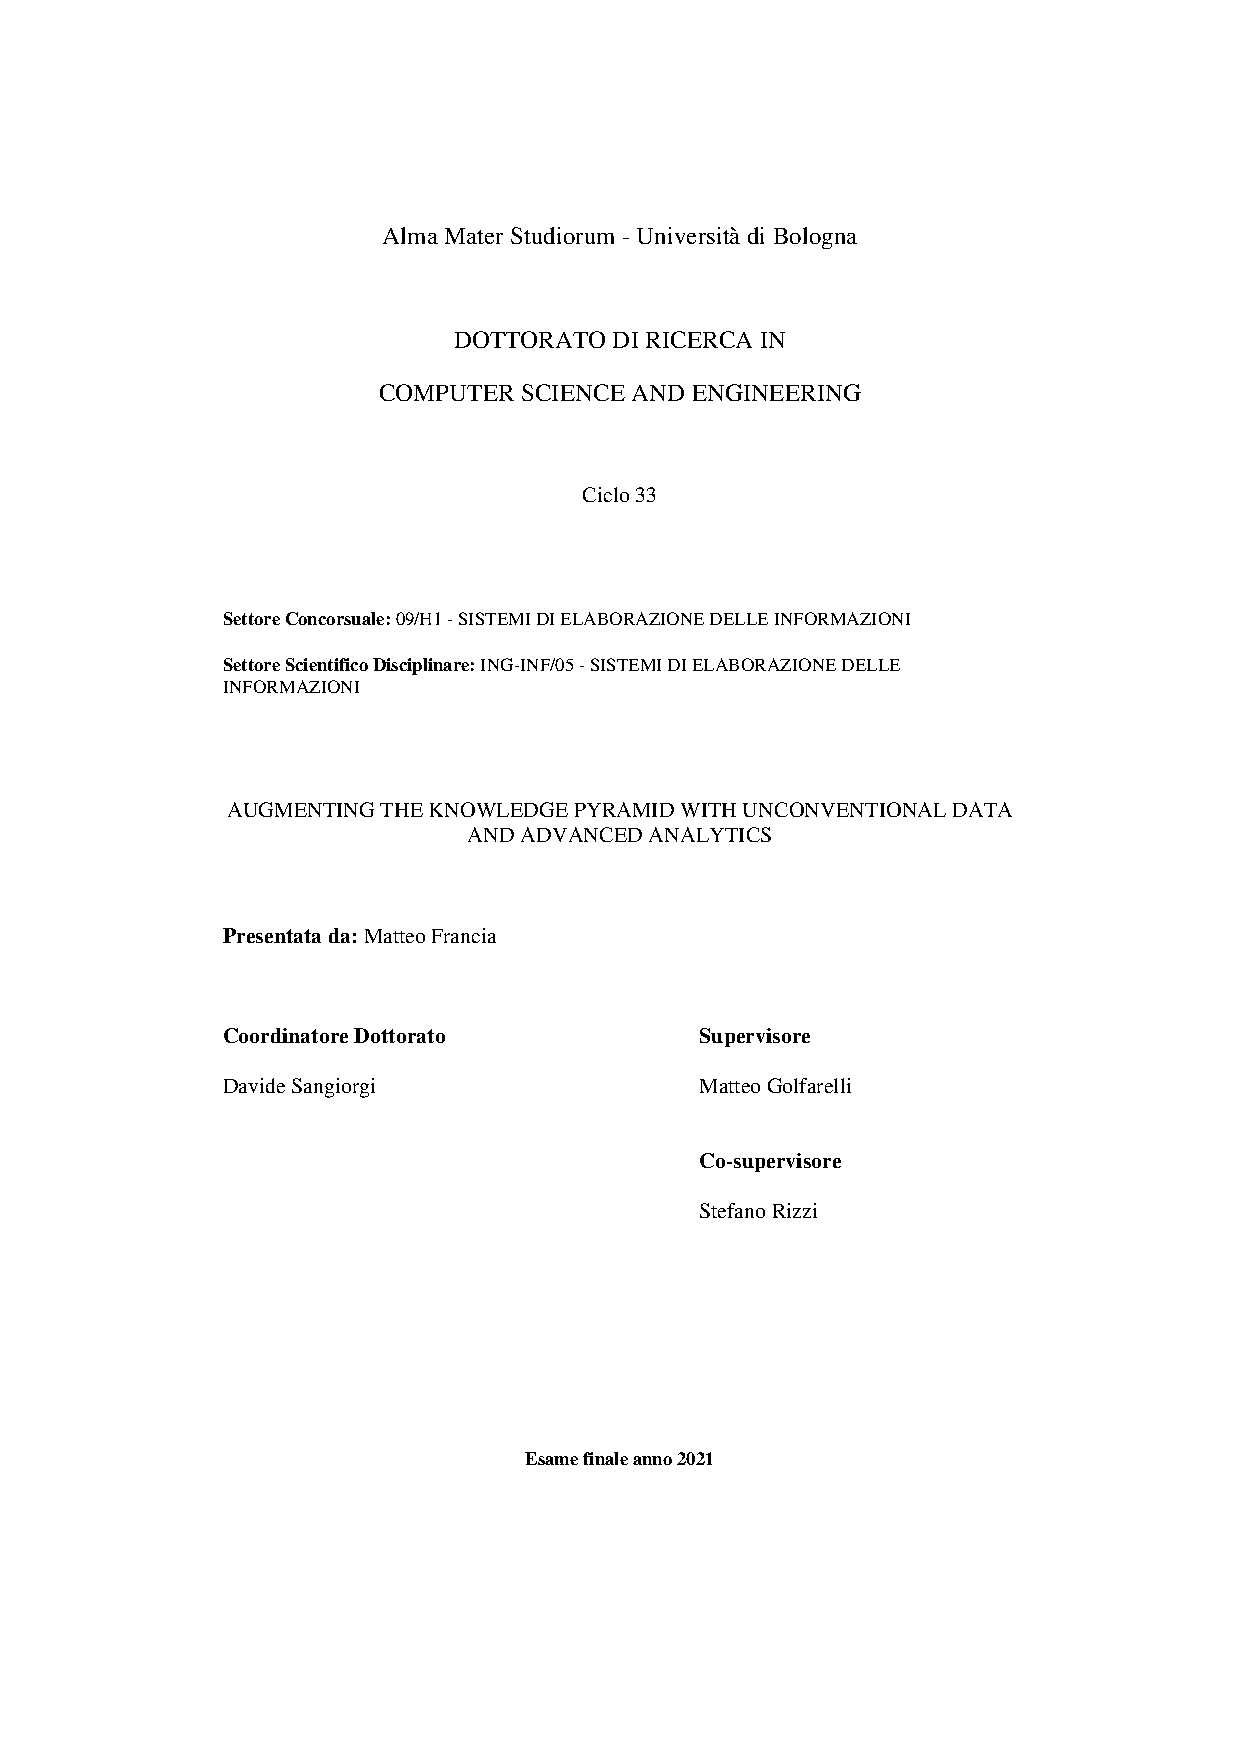
\includepdf[pages=-]{global/frontespizio.pdf}
\newpage
% \includepdf[pages=-]{global/researchactivity.pdf}
% ******************************* Thesis Dedication ********************************
\begin{dedication} 
\epigraph{\textit{``Quote needed''}}{}
\vspace{30mm}
To \dots.
\end{dedication}


% \include{global/declaration}
\include{global/quote}
\begin{acknowledgements}
\addcontentsline{toc}{chapter}{Acknowledgements}

Before diving into the depths of my research, I would like to acknowledge the sung and unsung heroes of this PhD journey.

\vspace{0.2cm}

% I would like to express my sincere gratitude to my advisors Prof. Matteo Golfarelli and Prof. Stefano Rizzi for their support and inspiration.
% My Ph.D. has been a joyful journey under their supervision.\\
The success of this thesis is certainly due to my research group, the business intelligence group (BIG).
First of all, I would like to thank my supervisor Prof. Matteo Golfarelli, who motivated me in the first place to start this PhD, and provided constant support and feedback.
I express my sincere gratitude to Prof. Stefano Rizzi for his priceless advice and encouragement.
I would like to thank my advisor Dr. Matteo Francia for his invaluable guidance, but also for welcoming me to the group ``so nicely''.
As to countless cups of coffee and \emph{italian passeggiate}, I thank my lab mates Dr. Enrico Gallinucci, Chiara Forresi, Manuele Pasini, Anna Giulia Leoni, Nicola Santolini, and Sterenn Roux.

\noindent At the Universitat Polit\`{e}cnica de Catalunya, Barcelona, huge thanks go to Prof. Alberto Abelló and Dr. Besim Bilalli for their inspiration and support during my Master's thesis, and throughout the whole PhD.

\noindent From Leibniz University, Hanover, I want to thank the AutoML group.
I would like to express my sincere gratitude to Prof. Marius Lindauer and Dr. Alexander Tornede, not only for the endless research insights and opportunities, but also for their kindness in welcoming me to the group.
Besides, I am grateful to have found an incredible group with which I had an amazing time.
I would like to thank Carolin Benjamins, Difan Deng, Theresa Eimer, Helena Graf, Aditya Mohan, Tim Ruhkopf, Sarah Segel, Daphne Theodorakopoulos, and Tanja Tornede.

\vspace{0.2cm}

With no doubts, I must thank my friends who both supported me during the ups and downs, and celebrated my achievements.
I would like to thank Gianluca Aguzzi,  Matteo Magnani, and Giuseppe Pisano.
I sincerely would not change anyone of you on this journey.
I would like to thank all the friends encountered during these years at the Cesena campus, especially in the Area 4.0 lab.
I believe the are not many groups having such a bond (and fun).
Especially, I would like to thank Giovanni Ciatto, Nicolas Farabegoli, Angela Cortecchia, Davide Domini, Matteo Magnini, Danilo Pianini, Martina Baiardi, Stefano Novellani, and Ruslan Shaiakhmetov.

\noindent My biggest thanks go to my mum Emilia for her never-ending support, solely a true \emph{mammone} can understand how much she means to me.
No less, I thank my father Renato and brother Yuri, for their continuous encouragement and for believing in me.

\noindent Last but not least, I would thank my partner Maria for cheering me up when ``it is not the day'', for her every-day caring, for all the fun, but -- mostly -- for always making me feel loved.

\end{acknowledgements}

\begin{abstract}

    % Riding the wave of recent groundbreaking achievements, artificial intelligence (AI) is currently the buzzword on everybody's lips and, building upon the notion of intelligence as learning, Machine Learning (ML) emerged as its pinnacle.
    % Riding the wave of recent groundbreaking achievements, artificial intelligence (AI) is currently the buzzword on everybody's lips and, addressing problems where human-crafted solutions are unfeasible, Machine Learning (ML) emerged as its pinnacle.
    % Artificial Intelligence (AI) stands as a transformative force, riding the wave of recent groundbreaking achievements, and Machine Learning (ML) emerged as its pinnacle, addressing problems where human-crafted algorithms are unfeasible and allowing algorithms to learn from historical data and discover solutions autonomously.
    % In particular, it addresses problems where human-crafted algorithms are unfeasible, allowing algorithms to learn from historical data and discover solutions autonomously.
    Riding the wave of recent groundbreaking achievements, artificial intelligence (AI) is currently the buzzword on everybody's lips and, allowing algorithms to learn from historical data, Machine Learning (ML) emerged as its pinnacle.
    The multitude of algorithms, each with unique strengths and weaknesses, highlights the absence of a universal solution and poses a challenging optimization problem.
    In response, automated machine learning (AutoML) navigates vast search spaces within minimal time constraints.
    By lowering entry barriers, AutoML emerged as promising the democratization of AI, yet facing some challenges.

    In \textbf{data-centric AI}, the discipline of systematically engineering data used to build an AI system, the challenge of configuring data pipelines is rather simple.
    We devise a methodology for building effective data pre-processing pipelines in supervised learning as well as a data-centric AutoML solution for unsupervised learning.

    In \textbf{human-centric AI}, many current AutoML tools were not built around the user but rather around algorithmic ideas, raising ethical and social bias concerns.
    % Motivated by such a mitigation call, this thesis contributes to human-centered AutoML, aiming at complementing, instead of replacing, human intelligence.
    We contribute by deploying AutoML tools aiming at complementing, instead of replacing, human intelligence.
    In particular, we provide solutions for single-objective and multi-objective optimization and showcase the challenges and potential of novel interfaces featuring large language models.

    Finally, there are application areas that rely on numerical simulators,
    % with domain experts manually configuring them through several trials and errors.
    often related to earth observations, they tend to be particularly high-impact and address important challenges such as climate change and crop life cycles.
    We commit to coupling these physical simulators with (Auto)ML solutions towards a \textbf{physics-aware AI}.
    Specifically, in precision farming, we design a smart irrigation platform that: allows real-time monitoring of soil moisture, predicts future moisture values, and estimates water demand to schedule the irrigation.

    % starting from supervised and unsupervised learning. The former is provided with a ground
    % truth to drive the learning towards a user-specified objective function

    % for both supervised learnand unsupervised learning, a
    % towards a more human-centered AutoML process.
    % In particular,
    % This places a mitigation call a shift toward the human-centered paradigm
    % Enabling human intervention, translating into the need for a shift toward the human-centered paradigm.
    % pushed towards a more human-centered AutoML process aimed at complementing, instead of replacing, human intelligence.

\end{abstract}
\tableofcontents
% \listoffigures
% \listoftables
% \printnomenclature%[3em]

% ******************************** Main Matter *********************************
\mainmatter
\sloppy
% \chapter{The Knowledge Pyramid}
\begin{figure}[t]
    \centering
    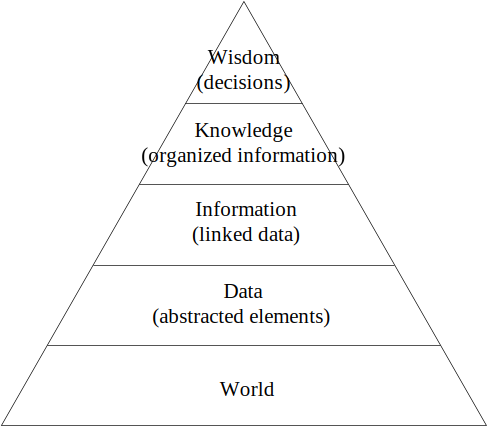
\includegraphics[scale=.7]{global/DIKW.pdf}
    \caption{The ``knowledge pyramid'' (also known as the ``Data Information Knowledge Wisdom pyramid'' or ``knowledge hierarchy''; adapted from \cite{DBLP:journals/oir/Stuart15b}).}
    \label{fig:dikw}
\end{figure}

Data science extracts actionable insights from raw data \cite{kelleher2018data}. The data transformation process is usually abstracted in the ``knowledge pyramid'' (also known as the ``Data Information Knowledge Wisdom pyramid'' or ``knowledge hierarchy''; \Cref{fig:dikw}), where data (i.e., symbols) are collected through measurements taken from the real world; information is processed and linked data that it is meaningful to scientists; knowledge is interpreted, understood, and organized information; and wisdom is knowledge in action. Climbing the pyramid is not a straightforward path and requires the iterative exploration and preparation of data so that patterns can be extracted, evaluated, and later deployed into models supporting effective decisions. 

Analytic applications strive to extract knowledge from data fueled by pervasive systems \cite{8423172}, where any device can be turned into a sensor leading to a huge volume and variety of available data \cite{vitali2021crop}. These \textit{unconventional}\footnote{We consider \textit{conventional} the data collected by operational databases, ERP (enterprise resource planning), and CRM (customer relationship management) enterprise systems} data (i.e., unstructured and non-relational data) have impacted on business intelligence (BI)---the discipline providing strategies and technologies to transform data into decision-making information---leading to BI 2.0, where decisions are drawn \textit{not only} on the data owned by the organization. Indeed, bigger data volumes lead to a holistic view of historic and current trends; higher data velocities ground decisions in continuously updated data, and broader data varieties provide many nuances of the matter at hand \cite{IBM4V}. On the one hand, volume and variety hinder the management, the integration, and the analysis of the collected data (from ``World'' to ``Data'' in \Cref{fig:dikw}), since each instance of unstructured data might have a different structure. This requires ad-hoc techniques for different data types (e.g., social networks \cite{DBLP:journals/snam/FranciaGG19} or sensor data \cite{DBLP:conf/mipro/FranciaGV19}). On the other hand, high availability has attracted scientists with no expertise in computer science or data engineering, requiring novel paradigms to support the ``Data''-to-``Knowledge''
%\footnote{Since ``wisdom'' is related to the \textit{application} of knowledge \cite{8423172}---besides no strict definition is given in the literature---we address the transformation of raw data into knowledge (i.e., patterns extracted with mining/machine learning models).} 
transformation with a higher abstraction level than formal programming languages (e.g., through graphical metaphors, recommender systems, or automatic transformation pipelines). Additionally, availability has enabled pervasive analyses, allowing data scientists to access data in hand-free contexts involving augmented reality and smart assistants.

While investigating these challenges, this thesis evolves into two parts.

\begin{figure}[t]
    \centering
    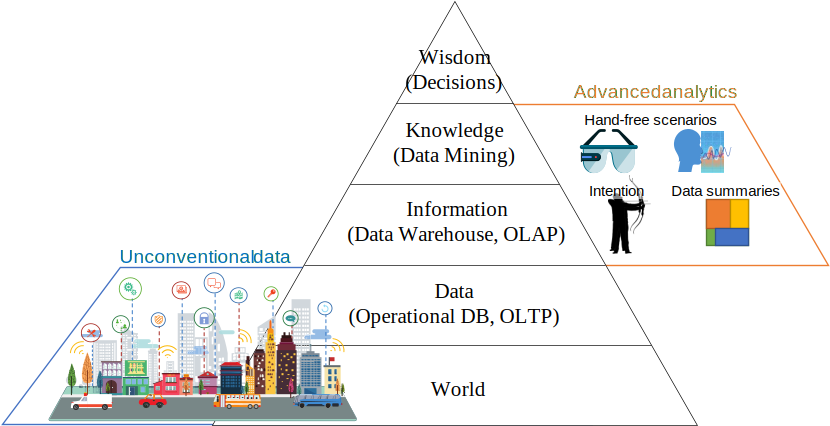
\includegraphics[scale=.65]{global/augmenting.pdf}
    \caption{Augmenting the knowledge pyramid with unconventional data (left) and advanced analytics (right).}
    \label{fig:aug}
\end{figure}

\paragraph{\Cref{part:trajectory}: Unconventional Data.}
Sensing provides real-time data upon which ``contextual'' decisions---ranging from user-centered to societal problems---are based. This includes data collected from human and technological assets (e.g., sensor or mobile networks), which are analyzed to monitor and manage urban and rural areas. Sensor data are highly available due to the growth of Internet of Things devices, have variable content, and their value comes from historic trends that range from hours to years \cite{kelleher2018data}. Such volume and variety demand for augmenting the knowledge pyramid with novel and scalable techniques for different data types (\Cref{fig:aug}). In urban mobility, spatiotemporal data (i.e., temporal sequences of spatial locations traced by moving objects and sampled through global or relative positioning sensors) are collected and processed for the sake of traffic analysis and forecasting, clustering of objects moving in similar paths, and habits profiling. Spatiotemporal data are challenging because of their uncertain, sparse, and multiresolution nature \cite{DBLP:journals/cacm/GilPBBBBCEGHHHK19}. Also, due to the number of moving objects (e.g., mobile devices, cars, taxis, and public transport in a metropolitan area) and to the sampling rate of positioning sensors (e.g., from minutes to seconds), mining mobility data easily scale up to big-data problems that require big-data solutions, hence introducing %a 
new business opportunities
% to analyze and extract information from data 
that were previously ignored because of technology limitations. Besides the valuable knowledge, due to high uniqueness \cite{DeMontjoye2013} and sensitivity (e.g., home and work locations), trajectory data expose individuals to privacy violations, demanding for ad-hoc techniques to (de-)anonymize historical trajectory datasets. In this direction, \Cref{part:trajectory} focuses on trajectory data and on the privacy implications of the publication of long-term mobility datasets.

\paragraph{\Cref{part:olap}: Advanced Analytics.}
Since the introduction of the relational model in the '70s, users used relational queries (e.g., SQL queries) to retrieve data collected in operational databases. This requires a good comprehension of programming languages and database management systems. Later, more user-friendly abstractions and tools provided a simpler view of the data, hiding the complexity of the underlying databases \cite{DBLP:journals/is/VassiliadisMR19} and transitioning from static (repetitive) workloads involving a few records (On-Line Transaction Processing, OLTP) to dynamic workloads (On-Line Analytical Processing, OLAP, and On-Line Analytical Mining, OLAM) involving a huge amount of records (\Cref{fig:aug}). The spread of data and analytical tools at hand has brought an increasing participation of data scientists with high competence in the business domain but low competence in computer science and data engineering \cite{DBLP:journals/is/VassiliadisMR19}. Indeed, data science emerged as an amalgamation of domain expertise with disciplines such as statistics, data mining, and databases \cite{vanderAalst2016}. Such amalgamation has brought challenges not only concerning big data volumes but also in terms of the increasing complexity and interdisciplinarity of the analytic questions. Enabling an effective participation in data science requires the investigation of user-centered paradigms supporting analytical querying and making knowledge extraction more accessible. Data scientists can benefit from proactive systems that ``understand'' the tasks at hand, make recommendations, and generate effective visualizations \cite{DBLP:journals/cacm/GilPBBBBCEGHHHK19}. For instance, in the digital twin scenario \cite{tao2018digital} where physical entities are mapped into a digital world, the synergy of personal assistants and augmented reality lacks analytic capabilities. Additionally, limited attention has been devoted to providing analytical reports that can be useful to let the user compare the current behavior of the visualized objects with their historical behavior. To this end, unconventional data sources, such as smart glasses and wearable devices, can be accessed by personal assistants (e.g., recommender systems) to address users' needs \cite{DBLP:conf/ictir/BahrainianC17}. Data scientists can interact with personal assistants through natural language interfaces which provide a higher abstraction level than formal queries and programming languages. In this direction, \Cref{part:olap} focuses on supporting data scientists with higher analytic abstractions than formal queries also in scenarios entailing pervasive data access. 

\chapter*{Introduction}

Artificial intelligence (AI) is currently the buzzword on everybody's lips.
Riding the wave of recent groundbreaking achievements, from self-driving cars \citep{} to intelligent chatbots \citep{}, AI is transforming industries and reshaping our daily lives.
Several interpretations and definitions have been provided over the years, yet the seminal perspective given by the Turing test \citep{turing1980computing} is still one worth mentioning.
\begin{definition}[Artificial Intelligence \citep{turing1980computing}]
A machine that shows intelligence indistinguishable from that of human beings is qualified to be labeled as artificial intelligence.
\end{definition}
This translates into understanding what falls under the umbrella of \textit{intelligence}, which is defined differently across the research areas as reasoning, planning, and learning.

\begin{definition}[Machine Learning \citep{samuel2000some}]
A machine with the ability to learn without being explicitly programmed.
\end{definition}
Building upon the notion of intelligence as learning, i.e. Machine Learning (ML), emerged as the pinnacle of AI due to its disruptive advancements.
At its core, ML aims at addressing problems for which the development of algorithms by humans is not feasible, because the algorithm itself is either not known or cost-prohibitive.
Examples include face recognition, fraud detection, sale forecasting, and object ranking. 
The problems are solved instead by letting the algorithms (e.g., neural networks \cite{}) \textit{discover their own solutions}: they perform a training process atop a sample of historical data, borrowing techniques from disciplines such as numerical analysis, statistics, and information theory.
The training process consists of fitting internal parameters (e.g., weights and bias) and providing ML practitioners with a model, which is ready to ingest new data and tackle the problem at hand.

There exists a plethora of different algorithms solving the same problem with different strengths and weaknesses, confirming theoretical results proving that there is \textit{no silver bullet} \cite{kerschke2019automated}---no algorithm dominates all others in all respects.
Besides, algorithms often expose some hyperparameters controlling the learning behavior (e.g., learning rate). 
To unleash the full potential of ML, practitioners have to carefully tune such hyperparameters but get easily overwhelmed by the showcased problem of combined algorithm selection and hyperparameter (CASH) optimization.

Automated machine learning (AutoML) demonstrates to play a crucial role in this landscape by tackling the CASH problem and, going beyond, by handling ever-larger search spaces in surprisingly small time budgets \cite{}.
Remarkable milestones include bayesian optimization (BO) to explore promising configurations based on prior evaluations,
meta-learning (i.e., learning atop learning) to warm-start BO (i.e., to boost the convergence process) by suggesting configurations that worked well in previous similar cases, and multi-fidelity methods to partially evaluate time-consuming configurations.
Besides, off-the-shelf solutions \cite{} are provided to tune entire ML pipelines, achieving -- in some cases -- higher performance than experts.

By lowering the barrier of access, AutoML emerged as promising for democratization of AI, i.e. making it accessible to both experts and non-experts alike.
Yet, when it comes to real-case scenarios, the journey of learning is riddled with challenges, ranging from the need for human intervention to mitigate harnessing, to the need for physical simulators.
% and heterogeneity of the data to constraints that may apply to the problem, from need for domain knowledge to .
While \Cref{chap:background} provides the necessary background, the remaining of the thesis investigates these challenges evolving into two parts.




\paragraph{Part I: Human-centered AutoML}

The original promise of AutoML was to automate certain ML tasks to a significant extent, thereby democratizing it and enabling non-experts to apply it in their respective domains.
However, despite their success, many current AutoML tools were not built around the user but rather around algorithmic ideas.
The stacking of complex mechanisms on top of each other unavoidably led to a less understanding of the process by the user -- even ML experts -- and allowing for very limited interaction.
Parts of the community have hence pushed towards a more human-centered AutoML process aimed at complementing, instead of replacing, human intelligence.
% This becomes even more crucial nowadays
% Motivated by ethical concerns and social bias issues arising at each step of the ML process, this becomes imperative in such a mitigating call nowadays.
Besides, motivated by ethical concerns and social bias issues arising at each step of the ML process, this approach becomes even imperative in such a mitigating call nowadays.
By placing the user back in the loop, it would be possible to revise and supervise the entire process, ensuring fairness, transparency, and ethical compliance.

In this part, we focus on the following contributions.
\begin{itemize}
    \item Providing the AutoML formalization to explicitly deal with thorough pipelines i.e., concatenations of pre-processing transformations and ML algorithms.
    \item Devising human-centered solutions for the main categories of ML i.e., supervised and unsupervised learning. The former is provided with a ground truth to drive the learning towards a user-specified objective function, the latter is by nature exploratory -- does not benefit from any ground truth -- and optimizing an objective is even more challenging.
    \item Addressing multi-objective ML, i.e. optimization of more than one loss or objective function, by interactively learning user preferences and drive the optimization towards it.
    \item Showcasing potential challenges, opportunities, and risks of novel (human-centered) AutoML interfaces with large language models (LLMs), i.e. AI models trained on large corpora of text to understand and produce human-like answers.
\end{itemize}

We organize this part as follows.
\Cref{automl-chap:formalization} provides the comprehensive AutoML formalization for ML pipelines.
\Cref{automl-chap:supervised} and \Cref{automl-chap:unsupervised} address supervised and unsupervised learning respectively.
\Cref{automl-chap:moo} delves into multi-objective ML and, lastly, \Cref{automl-chap:llm} discusses the novel human-centered AutoML interfaces with LLMs.
% In this part, we devise human-centered AutoML solutions for the main categories of ML.
% While in \Cref{automl-chap:formalization} we provide the AutoML formalization to explicitly deal with thorough pipelines i.e., concatenations of pre-processing transformations and ML algorithms, \Cref{automl-chap:supervised} and \Cref{automl-chap:unsupervised} address supervised and unsupervised learning respectively.
% The former is provided with a ground truth to drive the learning towards a user-specified objective function, the latter is by nature exploratory -- does not benefit from any ground truth -- and optimizing an objective is even more challenging.
% Then, \Cref{automl-chap:moo} delves into multi-objective ML, i.e. optimization of more than one loss or objective function.
% Lastly, \Cref{automl-chap:llm} showcases the potential challenges, opportunities, and risks of novel (human-centered) AutoML interfaces with large language models, i.e. AI models trained on large corpora of text to understand and produce human-like answers.

\paragraph{Part II: Physics-coupled AutoML}

As application areas go, there are domains in which ML models are not yet widespread.
Usually related to earth observations, the deployed applications tend to be particularly high-impact, trying to mitigate challenges such as climate change by delivering (more) eco-friendly systems.
Examples include weather forecasts and crop life-cycle management.
Domain experts leverage their knowledge to tune numerical simulators -- which encode well-known physical laws -- and deliver forecasts and analyses.
However, this process faces several challenges.
% several issues jeopardize this process.
The non-existence of universal well-defined practices translates to several trials and errors, with domain experts manually configuring the simulator parameters until an acceptable solution is found.
Yet, as variables involved in physics phenomena are subject to constant change, such numerical solution must undergo periodic (re-)calibration.
Besides, with the torrent of remotely sensed data available today, opportunities to integrate real-time observations in predictive models have emerged that traditional methods are not equipped to handle.
This is where advances in AI can push forward to enhance our understanding, provide support and, if necessary, steer the course of resolving global concerns to a more favorable future.
For instance, ML models exhibit singular performance in adapting themselves to handle scenarios different from the one they were trained on (e.g., fine-tuning of network parameters) and AutoML can significantly impact in automating several stages (e.g., tuning simulators and ML models).
% At the same time, relying on fully-automated data-driven methods for problems as complex and impactful as these is doomed to result in biased and unreliable.
% This underscores the ongoing importance of domain experts in this endeavor, highlighting their crucial role, with AI serving as a powerful tool.
% This is why domain experts, as always, remain crucial in this process, and why AI should be there as a powerful tool that supports them in fully taking advantage of the new opportunities we are presented with.

In this part, we focus on precision farming, which plays a pivotal role in addressing water wastage and improving crop efficiency.
\Cref{precision-chap:background} provides the necessary background and formalization in precision farming.
\Cref{precision-chap:architecture} overviews the architecture of our big-data smart-irrigation platform.
\Cref{precision-chap:orchard} deepens on Orchard3D-Lab, a well-known crop and soil simulator enhanced with auto-tuning and data assimilation capabilities, i.e. ingestion of sensor data for more reliable estimations.
\Cref{precision-chap:pluto} and \Cref{precision-chap:forecasting} delve -- respectively -- into the modules of real-time soil moisture monitoring and forecasting.
Finally, \Cref{precision-chap:smart-irrigation} deepens the smart-irrigation algorithm.


\chapter{Background}
\label{chap:background}

Alan Turing defines the field of AI in cognitive terms \cite{turing1980computing}, raising the question of whether machines can show intelligence, and along this line Arthur Samuel defines ML \cite{samuel2000some}, building upon the notion of intelligence as learning.
A more formal definition is provided by Tom M. Mitchell \citep{mitchell1997machine}, who delineates the behavior of algorithms studied in machine learning and introduces the concepts of \textit{task} and \textit{experience}.
\begin{definition}[Machine Learning \citep{mitchell1997machine}]
    A computer program is said to learn in some class of tasks, with respect to a performance measure, if its performance improves with experience.
\end{definition}
Notably, the formalization of experience is contingent upon the task to address, which is crucial because determines what the ML algorithm can observe and, in turn, how it operates.
Specifically, the literature identifies three different ML tasks: \textit{supervised}, \textit{unsupervised}, and \textit{reinforcement learning}.

\paragraph{Supervised learning} This is the kind of learning studied in most current research in the ML field. The algorithm is provided with a sample of data describing scenarios that have been \textit{experienced} in the past along with the corresponding \textit{ground truth}---i.e., values that indicate the correct outcomes.
The goal consists of finding a \textit{function} that maps samples to outcomes so that the next unseen scenarios can be labeled correctly.


\paragraph{Unupervised learning}
Here, the samples come with no ground truth available.
The algorithm has to guess the outcome by uncovering hidden insights or patterns, investigating different partitionings, or estimating density distributions within the data.
Analogously, tasks can be further categorized.
\begin{itemize}
    \item \textbf{Clustering} or \textbf{cluster analysis} tasks, when the outcome can assume finite values and it refers to the group that better represents the instances e.g., identifying customer segments based on purchasing behavior.
    \item Otherwise, the nomenclature usually comes after the task semantic e.g., anomaly detection assigns an outlier score to each instance that deviates from the overall distribution.
\end{itemize}
% Unsupervised tasks are inherently exploratory in nature and are often employed in data mining to provide explanations for the given scenarios or even to summarize them.

\paragraph{Reinforcement Learning}
Standing on the edge of the ML landscape, it has been categorized as the learning that differentiates the most from ``classical'' tasks \cite{sutton2018reinforcement}.
Here the experience is not sampled and fed to the algorithm but rather comes from interactions with an environment.
The algorithm learns by making decisions and receiving feedback based on its actions, allowing it to adapt its behavior over time.\\

%TODO: Qua c'è da menzionare che infatti automatizzare RL, in letteratura, prende il nome di AutoRL mentre noi facciamo AutoML.
This thesis focuses on supervised and unsupervised learning.
% providing a formalization that covers both cases.
Particularly in this chapter, \Cref{automl-background-sec:ml} introduces the building blocks such as dataset, algorithm, and hyperparameter; while
% provides the necessary background in ML,
\Cref{automl-background-sec:automl} formalizes the problems tackled by automated machine learning (AutoML), up to the combined algorithm selection and hyperparameter optimization.
% along with the state-of-the-art techniques to solve them.
% and finally \Cref{automl-background-sec:formalization} extends the formalization towards a more operational level of ML, enabling the user to handle comprehensive ML pipelines---i.e., concatenations of steps that cover more than the sole learning process.
% Here we can also put something like " ... extends the formalization focusing on a more operational level of ML and methods that following this way enables to handle comprehensive ... "

\section{Machine Learning}\label{automl-background-sec:ml}

At the core of each and every task lies the data, serving as the essential fuel for the learning process because providing the means to observe the real world.
Specifically in ML, we refer to a dataset $\altmathcal{D}$ as a sample of data from which it is possible to learn that experience of interest.

\begin{definition}[Dataset]\label{def:dataset}
    A \textit{dataset} $\altmathcal{D}$ is a collection of data points $X$, with corresponding space $\altmathcal{X}$.
    According to the task $T$, the dataset may include the ground truth $Y$ within its corresponding space $\altmathcal{Y}$ (supervised) or not (unsupervised).
    \begin{equation*}\label{eq:dataset}
        \altmathcal{D} = \left\lbrace\,
        \begin{array}{@{}l@{}l@{\quad}l@{}}
            (\pmb{x}_i, y_i)_{i=1}^N & \in \mathbb{D} \subset \altmathcal{X} \times \altmathcal{Y} & \text{{if }} T = \text{{supervised}} \\
            (\pmb{x}_i)_{i=1}^N & \in \mathbb{D} \subset \altmathcal{X} & \text{{if }} T = \text{{unsupervised}}
        \end{array}
        \right.
    \end{equation*}
\end{definition}

Intuitively, a dataset resembles a structured table where each row represents a unique instance $x \in X$ characterized by specific features in their domain $\altmathcal{X}$.
The features, denoted by the columns, describe the diverse factors or characteristics influencing a particular outcome $Y$ in its domain $\altmathcal{Y}$.
While in supervised learning the ground truth is provided with the aim of understanding the hidden relationships between features and corresponding outcomes, in supervised tasks, the most appropriate outcome has to be found by discovering patterns within the data.

\begin{example}[Iris dataset \cite{iris}]\label{ex:dataset}
    The iris dataset contains $150$ instances of flowers ($X$) under four features in cm ($\altmathcal{X} \subset \mathbb{R}^4$): sepal length, sepal width, petal length, and petal width.
    The data have been collected to quantify the morphologic variation within the Iris species ($Y$), which can assume the following $3$ classes ($\altmathcal{Y}$): Iris setosa, Iris virginica and Iris versicolor.
    \begin{table}[!h]
        \centering
        \begin{tabular}{llll|l}
            \hline
            Sepal length & Sepal width & Petal length & Petal width & Class \\ \hline
            % $5.1$ & $3.5$ & $1.4$ & $0.2$ & Iris-setosa \\
            $4.9$ & $3.0$ & $1.4$ & $0.2$ & Iris-setosa \\
            % $7.0$ & $3.2$ & $4.7$ & $1.4$ & Iris-versicolor \\
            $6.4$ & $3.2$ & $4.5$ & $1.5$ & Iris-versicolor \\
            % $6.3$ & $3.3$ & $6.0$ & $2.5$ & Iris-virginica \\
            $5.8$ & $2.7$ & $5.1$ & $1.9$ & Iris-virginica \\ \hline
            \
        \end{tabular}
        \caption{Example tuples from the Iris dataset.}
        \label{tbl:iris}
    \end{table}

    \noindent This dataset is also used in unsupervised learning tasks by discarding the class attribute, yet the data only contains two clusters with rather obvious separation.
\end{example}

% The aim is to discover the hidden relationships between inputs $X$ and outputs $Y$, hence learning a function $f: \altmathcal{X} \rightarrow \altmathcal{Y}$.
% Despite the task,
The ultimate goal is learning a function $f: \altmathcal{X} \rightarrow \altmathcal{Y}$.
A (machine) learning \textit{algorithm} $A$ leverages data points in $\altmathcal{D}$ to estimate such a function $f$, which is expressed via a vector of \textit{model parameters} $H$.
Most algorithms further expose hyperparameters $\lambda_1, \dots, \lambda_K$ that change the functioning of the algorithm itself.

\begin{definition}[Machine Learning Algorithm]\label{def:algorithm}
    Given a dataset $\altmathcal{D}$ and a hyperparameter space $\pmb{\Lambda}$, an algorithm $A$ provides a model $H$ from the model space $\altmathcal{H}$.
    \begin{equation*}\label{eq:algorithm}
        A: \mathbb{D} \times \pmb{\Lambda} \rightarrow \altmathcal{H}
    \end{equation*}
    Given the hyperparameters $\lambda_1, \dots, \lambda_M$, with corresponding spaces $\Lambda_1, \dots, \Lambda_M$, we refer with $\pmb{\lambda}$ to a hyperpaprameter configuration sampled from the space $\pmb{\Lambda} = \Lambda_1 \times \dots \times \Lambda_M$.
\end{definition}

The actual learning is performed via the so-called \textit{model training} or, due to the iterative process of adjusting internal parameters until convergence, \textit{model fitting}.
The quality of such a model heavily depends on the hyperparameter choices we made, hence we need loss functions that assess the quality of different configurations.
% How well a model performs depends heavily on the hyperparameter choices we make and loss functions assess the quality of such configurations.
The term loss typically refers to the error committed by the model, hence the lower the better; instead, when higher values are favored, we refer to quality metrics.
Quality metrics share the same signature as the losses.

\begin{definition}[Loss Function]\label{def:loss}
    Given a dataset $\altmathcal{D}$ and a model $H$, the loss function $\altmathcal{L}$ quantifies how well the given model performs on $\altmathcal{D}$.
    \begin{equation*}\label{eq:loss}
        \altmathcal{L}: \altmathcal{H} \times \mathbb{D} \rightarrow \mathbb{R}
    \end{equation*}
\end{definition}

In the following, we walk over the main characteristics and differences between the specific cases of supervised and unsupervised learning.

\subsection{Supervised Learning}

First of all, supervised learning can be further differentiated based on the nature of the desired outcome.
\begin{itemize}
    \item \textbf{Classification} tasks, when the outcome can assume finite values and it represents the class to which the instances belong e.g., in an image recognition use-case: ``dog'', ``cat'', ``car'', or ``tree''.
    \item \textbf{Regression} tasks, when the outcome is continuous e.g., predicting house prices, stock prices, or temperature.
\end{itemize}
This might alter how some algorithms internally work but, for our perspective, they are still designed to be fed with a labeled dataset and, through model training, to minimize the discrepancy between its predictions and actual outcomes.
The ultimate goal is to deploy a model that performs well on new data, hence achieving a good \textit{generalization}.
Yet, two undesired scenarios can occur.
\textit{Overfitting} takes place when the model is too complex and fits the training data too closely, not being able to generalize the acquired knowledge to unseen data and capturing noise rather than genuine patterns.
On the contrary, \textit{underfitting} happens when a model is too simplistic, failing to capture the underlying complexities.
Hyperparameters are crucial in striking the right balance.

\begin{example}[Decision Tree]
    The decision tree algorithm recursively splits instances based on their feature values, creating a hierarchical tree-like structure where each leaf represents a class or a prediction value---in classification and regression tasks respectively.
    % Notably, in its supervised nature, the tree can be built by minimizing the entropy of the leaves.
    We can control the complexity of such a tree by leveraging hyperparameters such as the maximum depth of the tree and the minimum number of instances in the leaves.
    In this case, a deeper tree with more splits may capture intricate patterns but is prone to overfitting, as to a shallower tree, it might generalize better but may overlook finer details.
\end{example}

Loss functions are inevitable when it comes to assess generalization performance but their application should also follow protocols that assure consistency and statistical reliability.
The most common protocol involves splitting the original dataset $\altmathcal{D}$ into two disjoint sets $\altmathcal{D}_\mathit{train}$ and $\altmathcal{D}_\mathit{valid}$, where the model is trained only based on $\altmathcal{D}_\mathit{train}$ but validated with $\altmathcal{L}$ on $\altmathcal{D}_\mathit{valid}$.
Yet, both model training and validation demand substantial amounts of data.
When the split is not feasible, a practical solution is the $k$-fold cross-validation technique.
This divides the dataset into $k$ folds and, for each fold, uses the corresponding subset of data for testing while employing the remaining $(k - 1)$ folds for training.

\begin{definition}[$K$-Fold Cross-Validation]
    The $k$-fold cross-validation provides a protocol to validate an algorithm $A$ with corresponding hyperparameter configuration $\lambda$ via a loss $\altmathcal{L}$ on a dataset $\altmathcal{D}$.
    \begin{equation*}
        \frac{1}{k}~\mathlarger{\sum}_{i=1}^{k} \altmathcal{L}(A(\altmathcal{D}_{train}^{(i)}, \lambda), \altmathcal{D}_{valid}^{(i)})
    \end{equation*}
    where $\altmathcal{D}_{train}^{(i)} = \altmathcal{D} \setminus \altmathcal{D}_{valid}^{(i)}$.
\end{definition}

Follows two examples of losses: misclassification error (\Cref{ex:misclassification}) and root mean square error (\Cref{ex:rmse}), for classification and regression tasks respectively.

\begin{example}[Misclassification Error]\label{ex:misclassification}
    Given the validation set $(x, y) \in D_\mathit{valid}$  and the model $H$ resulted from the training $A(D_\mathit{train}, \lambda)$, then the loss MIS computes the fraction of incorrect predictions made by $H$.
    \begin{equation*}
        MIS(H, \altmathcal{D}_\mathit{valid}) = \frac{1}{|D_\mathit{valid}|}~\mathlarger{\sum}_{(x, y) \in D_\mathit{valid}} (H(x) \ne y)
    \end{equation*}
    In classification tasks, the accuracy ($ACC = 1 - MIS$) computes the fraction of incorrect predictions and is often used as a quality metric.
\end{example}


\begin{example}[Root Mean Square Error]\label{ex:rmse}
    Given the validation set $(x, y) \in D_\mathit{valid}$  and the model $H$ resulted from the training $A(D_\mathit{train}, \lambda)$, then the loss RMSE computes the average difference between the predictions made by $H$ and the actual values in $D_\mathit{valid}$.
    \begin{equation*}
        RMSE(H, \altmathcal{D}_\mathit{valid}) = \sqrt{\frac{1}{|D_\mathit{valid}|}~\mathlarger{\sum}_{(x, y) \in D_\mathit{valid}} (H(x) - y)^2}
    \end{equation*}
\end{example}

\subsection{Unsupervised Learning}

For unsupervised tasks: k-means \cite{} and isolation forest \cite{}.

\begin{example}[K-Means]
    The k-means algorithm aims to partition the instances into a predetermined number of clusters based on their feature similarity.
    Being unsupervised, the algorithm iteratively assigns instances to clusters and updates the cluster centroids until its convergence criteria i.e., instances in the same cluster are more similar than instances in a different cluster.
    Hyperparameters such as the number of clusters and the similarity measure affect the returned partitioning.
\end{example}

\section{Automated Machine Learning}\label{automl-background-sec:automl}


% \begin{itemize}
%     \item Qui ci va sicuramente la formalizzazione
%     \item la motivation è dubbia, forse ripeteremmo quello che è scritto sopra nell'Introduction
% \end{itemize}



\part{Human-centered AutoML}\label{part:automl}


\chapter{Formalization}\label{automl-chap:formalization}

% \chapter{Introduction}
\label{chap:intro}

Artificial intelligence (AI) is currently the buzzword on everybody's lips.
Riding the wave of recent groundbreaking achievements, from self-driving cars \citep{} to intelligent chatbots \citep{}, AI is transforming industries and reshaping our daily lives.
Several interpretations and definitions have been provided over the years, yet the seminal perspective given by the Turing test \citep{turing1980computing} is still one worth mentioning.
\begin{definition}[Artificial Intelligence \citep{turing1980computing}]
A machine that shows intelligence indistinguishable from that of human beings is qualified to be labeled as artificial intelligence.
\end{definition}
This translates into understanding what falls under the umbrella of \textit{intelligence}, which is defined differently across the research areas as reasoning, planning, and learning.
\begin{definition}[Machine Learning \citep{samuel2000some}]
A machine with the ability to learn without being explicitly programmed.
\end{definition}
Building upon the notion of intelligence as learning, i.e. Machine Learning (ML), emerged as the pinnacle of AI due to its disruptive advancements.
At its core, ML aims at addressing problems for which the development of algorithms by humans is not feasible, because the algorithm itself is either not known or cost-prohibitive.
Examples include face recognition, fraud detection, sale forecasting, and object ranking.
The problems are solved instead by letting the algorithms (e.g., neural networks \cite{nn}) \textit{discover their own solutions}: they perform a training process atop a sample of historical data, borrowing techniques from disciplines such as numerical analysis, statistics, and information theory.
The training process consists of fitting internal parameters (e.g., weights and bias) and providing practitioners with a model.
In this context, we can hence define an \textit{AI system} as the (software) solution that deploys an ML model specific for the problem at hand i.e., ready to ingest new data and tackle it.

There exists a plethora of different algorithms solving the same problem with different strengths and weaknesses, confirming theoretical results proving that there is \textit{no silver bullet} \cite{kerschke2019automated}---no algorithm dominates all others in all respects.
Besides, algorithms often expose some hyperparameters controlling the learning behavior (e.g., learning rate).
To unleash the full potential of ML, practitioners have to carefully tune such hyperparameters but get easily overwhelmed by the showcased problem of combined algorithm selection and hyperparameter (CASH) optimization.

Automated machine learning (AutoML) demonstrates to play a crucial role in this landscape by tackling the CASH problem and, going beyond, by handling ever-larger search spaces in surprisingly small time budgets \cite{small_time_budgets}.
Remarkable milestones include bayesian optimization (BO) to explore promising configurations based on prior evaluations,
meta-learning (i.e., learning atop learning) to warm-start BO (i.e., to boost the convergence process) by suggesting configurations that worked well in previous similar cases, and multi-fidelity methods to partially evaluate time-consuming configurations.
% Besides, off-the-shelf solutions \cite{auto_sklearn} are provided to tune entire ML pipelines, achieving -- in some cases -- higher performance than experts.
By lowering the barrier of access, AutoML emerged as promising for the democratization of AI, i.e. making it accessible to both experts and non-experts alike.
Yet, when it comes to real-case scenarios, the journey of
delivering AI systems
% learning
is riddled with challenges.

\begin{figure}
    \centering
    \includegraphics[scale=0.3]{chapters/chapter-introduction/img/contribution_overview.png}
    \caption{Contirbution Overview.}
    \label{fig:contribution}
\end{figure}

% ranging from the need for human intervention to mitigate harnessing, to the need for physical simulators.
Let us quickly overview the end-to-end process.
The main character is usually the data scientist, a specialist in machine learning and data analysis, which leverages a process model to translate the \textit{knowledge} about the problem into \textit{ML constraints} and deploy the system.
The cross-industry standard process for data mining \cite{wirth2000crisp} (CRISP-DM) is considered the open standard and we will take it as a reference in the whole thesis.
Given the numerous skills expected by data scientists,
their numbers fall short of the needs,
% their numbers cannot meet the needs,
% their number does not scale with the needs,
leading domain experts to carry out such a process.
For the sake of simplicity, we keep these two roles separated.
% is an open standard process model and standard de facto that guides the ML experts, better known as \textit{data scientists}, through the different stages in applied machine learning problems.
\textbf{Domain} and \textbf{data understanding} entail domain experts and the data scientist working in close cooperation to explore constraints and study available data, respectively.
% \textbf{Data understanding} is devoted to the study of the data collected, its semantics and transformations
These stages might be repeated many times until the data scientists are satisfied with the acquired knowledge.
Follows the iterative investigation of different solutions throughout \textbf{data pre-processing}, \textbf{modelling}, and \textbf{evaluation}.
Data pre-processing and modelling are conducted to build a data pipeline and train an ML algorithm, respectively.
More in detail, a series of pre-processing transformations shape the data so that the ML algorithm can output the best model.
Then, evaluation offers a way to measure the performance and the process can conclude with the \textbf{deployment} of the AI system, including the implementation of the running environment.
% ---i.e., the actual implementation of the solution.
% \textbf{Data pre-processing}, \textbf{modelling}, and \textbf{evaluation} are iteratively conducted to investigate different pipelines---i.e., series of pre-processing transformations that shape the data so that the ML algorithm can perform at its best.

\Cref{fig:contribution} shows the CRISP-DM process model and the research areas we focus on.
Specifically, according to challenges that are addressed: data-centric, human-centric, and physics-aware AI.
% According to the challenges that are addressed, this thesis contributes to three research areas.
% following research areas.
While \Cref{chap:background} provides the necessary background, the remaining of the thesis evolves in the corresponding three parts.
% Specifically, while \Cref{chap:background} provides the necessary background, the remaining of the thesis evolves in three parts.
% While \Cref{chap:background} provides the necessary background, the remaining of this thesis investigates these challenges evolving into two parts.


\paragraph{Part I: Data-centric AI}

During the past few decades, most of the efforts in AI were focused on improving ML algorithms, leading to numerous groundbreaking achievements.
In many applications, modelling is considered the solved part of the puzzle and the vast majority of the time is spent on improving the data.
Data-centric AI is the discipline of systematically engineering data used to build an AI system, yet the challenge of configuring data pipelines is rather simple.
A combinatorial space has to be explored, entailing ad-hoc pre-processing for the algorithm at hand, and constraints within data, transformations, and algorithms exacerbate the problem at hand.
While AutoML traditionally neglected data quality and pre-processing, there is an untapped potential to contribute to this research area.
Indeed, given the huge combinatorial space, AutoML can help in designing efficient AI systems with a meticulous focus on data.
% AI systems are made up of both code, which is software implementing the model or learning algorithm, as well as data, which you run the code on.
% Over the past few decades, most of the efforts in AI have focused on improving the code and the dominant paradigm in research was to download the dataset and hope the data is fixed while you work on the code.
% Thanks to all this innovation in the code, part of the puzzle for many applications, I find that the code is basically a solved problem.
% Data-centric AI is a shift toward developing software tools as well as entering practices to make improving the data efficient reliable and systematic in the last decade the biggest shift in AI was embracing deep learning in this decade.
% I think the biggest shift in AI might be a shift to data-centric AI.
% The resources on the site will allow you to take part in this next major trend for ai techniques and I'm excited for you to harness the power of these ideas to more quickly build successful AI systems you
% I think the biggest shift in AI might be a shift to data-centric AI.

% Yet, serving as the essential fuel for the learning process, data plays an even more crucial role.
% Data plays a key role in the ML process.

% It encompasses a broad range of activities that span from correcting errors to selecting the most relevant features for the analysis phase.
% There is no clear evidence, or rules defined, on how pre-processing transformations impact the final results of the analysis.
% The problem is exacerbated when transformations are combined into pre-processing pipelines.
% Data scientists cannot easily foresee the impact of pipelines and hence require a method to discriminate between them and find the most relevant ones (e.g., with the highest positive impact) for their study at hand.

In this part, we devise data-centric solutions for the main categories of ML i.e., supervised and unsupervised learning.
The former is provided with a ground truth to drive the learning towards a user-specified objective function, the latter is by nature exploratory -- does not benefit from any ground truth -- and optimizing an objective is even more challenging.
Specifically, we focus on the following contributions.
\begin{itemize}
    \item As to supervised learning, we study the impact of transformations when chained together into data pipelines and when instantiated via various operators.
    Then, we extract a set of rules according to their semantics and develop a generic method that allows the generation of efficient pipelines, leading to 90\% of the performance in the median, but with a time cost that is 24 times smaller.
    \item As to unsupervised learning, we focus on cluster analysis---i.e., partitioning the data such that items in the same cluster are more similar than those in different clusters.
    We design a framework that explores and returns a dashboard of both relevant and diverse partinionings via AutoML and diversification.
    AutoML ensures that the explored pipelines for cluster analysis (also including pre-processing steps) compute good clusterings.
    Then, diversification selects, out of the explored clusterings, the ones conveying different clues to the data scientists.
\end{itemize}

We supervised and unsupervised learning in \Cref{} and \Cref{}, respectively.

\paragraph{Part I: Human-centered AutoML}

The original promise of AutoML was to automate certain ML tasks to a significant extent, thereby democratizing it and enabling non-experts to apply it in their respective domains.
However, despite their success, many current AutoML tools were -- yet another time -- not built around the user but rather around algorithmic ideas.
The stacking of complex mechanisms on top of each other unavoidably led to a less understanding of the process -- even by ML experts -- and allowing for very limited interaction.
Parts of the community have hence pushed towards a more human-centered AutoML process aimed at complementing, instead of replacing, human intelligence.
% This becomes even more crucial nowadays
% Motivated by ethical concerns and social bias issues arising at each step of the ML process, this becomes imperative in such a mitigating call nowadays.
Besides, motivated by ethical concerns and social bias issues arising at each step of the ML process, this approach becomes even imperative in such a mitigating call nowadays.
By placing the user back in the loop, we let the user to revise and supervise the entire process, ensuring fairness, transparency, and ethical compliance.

In this part, we focus on the following contributions.
\begin{itemize}
    % \item Providing the AutoML formalization to explicitly deal with thorough pipelines i.e., concatenations of pre-processing transformations and ML algorithms.
    \item Devising a human-centered framework for supervised learning in a single-objective of a user-specified function.
    Specifically, we design a framework that enablesusers to express ML constraints in a uniformed human- and machine-readable medium.
    Constraints are interpreted to drive the AutoML exploration, which retrieves the most performing pipelines and, finally, new constraints are learned and integrated through logic and argumentation.
    \item Addressing multi-objective ML, i.e. optimization of more than one loss or objective function, by interactively learning user preferences and drive the optimization towards it.
    \item Showcasing potential challenges, opportunities, and risks of novel (human-centered) AutoML interfaces with large language models (LLMs), i.e. AI models trained on large corpora of text to understand and produce human-like answers.
\end{itemize}

We organize this part as follows.
% \Cref{automl-chap:formalization} provides the comprehensive AutoML formalization for ML pipelines.
\Cref{automl-chap:supervised} addresses the supervised single-objective optimization.
\Cref{automl-chap:moo} delves into multi-objective ML and, lastly, \Cref{automl-chap:llm} discusses the novel human-centered AutoML interfaces with LLMs.
% In this part, we devise human-centered AutoML solutions for the main categories of ML.
% While in \Cref{automl-chap:formalization} we provide the AutoML formalization to explicitly deal with thorough pipelines i.e., concatenations of pre-processing transformations and ML algorithms, \Cref{automl-chap:supervised} and \Cref{automl-chap:unsupervised} address supervised and unsupervised learning respectively.
% The former is provided with a ground truth to drive the learning towards a user-specified objective function, the latter is by nature exploratory -- does not benefit from any ground truth -- and optimizing an objective is even more challenging.
% Then, \Cref{automl-chap:moo} delves into multi-objective ML, i.e. optimization of more than one loss or objective function.
% Lastly, \Cref{automl-chap:llm} showcases the potential challenges, opportunities, and risks of novel (human-centered) AutoML interfaces with large language models, i.e. AI models trained on large corpora of text to understand and produce human-like answers.

\paragraph{Part II: Physics-coupled AutoML}

As application areas go, there are domains in which ML models are not yet widespread.
Usually related to earth observations, the deployed applications tend to be particularly high-impact, trying to mitigate challenges such as climate change by delivering (more) eco-friendly systems.
Examples include weather forecasts and crop life-cycle management.
Domain experts leverage their knowledge to tune numerical simulators -- which encode well-known physical laws -- and deliver forecasts and analyses.
However, this process faces several challenges.
% several issues jeopardize this process.
The non-existence of universal well-defined practices translates to several trials and errors, with domain experts manually configuring the simulator parameters until an acceptable solution is found.
Yet, as variables involved in physics phenomena are subject to constant change, such numerical solution must undergo periodic (re-)calibration.
Besides, with the torrent of remotely sensed data available today, opportunities to integrate real-time observations in predictive models have emerged that traditional methods are not equipped to handle.
This is where advances in AI can push forward to enhance our understanding, provide support and, if necessary, steer the course of resolving global concerns to a more favorable future.
For instance, ML models exhibit singular performance in adapting themselves to handle scenarios different from the one they were trained on (e.g., fine-tuning of network parameters) and AutoML can significantly impact in automating several stages (e.g., tuning simulators and ML models).
% At the same time, relying on fully-automated data-driven methods for problems as complex and impactful as these is doomed to result in biased and unreliable.
% This underscores the ongoing importance of domain experts in this endeavor, highlighting their crucial role, with AI serving as a powerful tool.
% This is why domain experts, as always, remain crucial in this process, and why AI should be there as a powerful tool that supports them in fully taking advantage of the new opportunities we are presented with.

In this part, we focus on precision farming, which plays a pivotal role in addressing water wastage and improving crop efficiency. Specifically, we commit to the following contributions.
\begin{itemize}
    \item Devising an extensive and flexible architecture for a big-data smart-irrigation platform that allows to perform analytics by coupling (automated) machine learning with physically-based models.
    \item Controlling soil moisture in real-time by relying on a grid of sensors and building fine-grained 2D and 3D profiles that enable a comprehensive analysis of the field.
    \item Forecasting the soil moisture through a two-stage optimization technique that also enables the system to adapt to new in-situ conditions.
    \item Providing a smart-irrigation approach that estimates the daily water amount needed by the plant and -- based on a grid of sensors and weather forecasts -- schedules the irrigation.
\end{itemize}



We organize this part as follows. \Cref{precision-chap:formalization} provides the necessary formalization in precision farming and overviews the designed architecture of our big-data smart-irrigation platform.
\Cref{precision-chap:orchard} deepens on Orchard3D-Lab, a well-known crop and soil simulator enhanced with auto-tuning and data assimilation capabilities, i.e. ingestion of sensor data for more reliable estimations.
\Cref{precision-chap:pluto} and \Cref{precision-chap:forecasting} delve -- respectively -- into the modules of real-time soil moisture monitoring and forecasting.
Finally, \Cref{precision-chap:smart-irrigation} deepens the smart-irrigation approach.
\chapter{Introduction}
\label{chap:intro}

Artificial intelligence (AI) is currently the buzzword on everybody's lips.
Riding the wave of recent groundbreaking achievements, from self-driving cars \citep{} to intelligent chatbots \citep{}, AI is transforming industries and reshaping our daily lives.
Several interpretations and definitions have been provided over the years, yet the seminal perspective given by the Turing test \citep{turing1980computing} is still one worth mentioning.
\begin{definition}[Artificial Intelligence \citep{turing1980computing}]
A machine that shows intelligence indistinguishable from that of human beings is qualified to be labeled as artificial intelligence.
\end{definition}
This translates into understanding what falls under the umbrella of \textit{intelligence}, which is defined differently across the research areas as reasoning, planning, and learning.
\begin{definition}[Machine Learning \citep{samuel2000some}]
A machine with the ability to learn without being explicitly programmed.
\end{definition}
Building upon the notion of intelligence as learning, i.e. Machine Learning (ML), emerged as the pinnacle of AI due to its disruptive advancements.
At its core, ML aims at addressing problems for which the development of algorithms by humans is not feasible, because the algorithm itself is either not known or cost-prohibitive.
Examples include face recognition, fraud detection, sale forecasting, and object ranking.
The problems are solved instead by letting the algorithms (e.g., neural networks \cite{nn}) \textit{discover their own solutions}: they perform a training process atop a sample of historical data, borrowing techniques from disciplines such as numerical analysis, statistics, and information theory.
The training process consists of fitting internal parameters (e.g., weights and bias) and providing practitioners with a model.
In this context, we can hence define an \textit{AI system} as the (software) solution that deploys an ML model specific for the problem at hand i.e., ready to ingest new data and tackle it.

There exists a plethora of different algorithms solving the same problem with different strengths and weaknesses, confirming theoretical results proving that there is \textit{no silver bullet} \cite{kerschke2019automated}---no algorithm dominates all others in all respects.
Besides, algorithms often expose some hyperparameters controlling the learning behavior (e.g., learning rate).
To unleash the full potential of ML, practitioners have to carefully tune such hyperparameters but get easily overwhelmed by the showcased problem of combined algorithm selection and hyperparameter (CASH) optimization.

Automated machine learning (AutoML) demonstrates to play a crucial role in this landscape by tackling the CASH problem and, going beyond, by handling ever-larger search spaces in surprisingly small time budgets \cite{small_time_budgets}.
Remarkable milestones include bayesian optimization (BO) to explore promising configurations based on prior evaluations,
meta-learning (i.e., learning atop learning) to warm-start BO (i.e., to boost the convergence process) by suggesting configurations that worked well in previous similar cases, and multi-fidelity methods to partially evaluate time-consuming configurations.
% Besides, off-the-shelf solutions \cite{auto_sklearn} are provided to tune entire ML pipelines, achieving -- in some cases -- higher performance than experts.
By lowering the barrier of access, AutoML emerged as promising for the democratization of AI, i.e. making it accessible to both experts and non-experts alike.
Yet, when it comes to real-case scenarios, the journey of
delivering AI systems
% learning
is riddled with challenges.

\begin{figure}
    \centering
    \includegraphics[scale=0.3]{chapters/chapter-introduction/img/contribution_overview.png}
    \caption{Contirbution Overview.}
    \label{fig:contribution}
\end{figure}

% ranging from the need for human intervention to mitigate harnessing, to the need for physical simulators.
Let us quickly overview the end-to-end process.
The main character is usually the data scientist, a specialist in machine learning and data analysis, which leverages a process model to translate the \textit{knowledge} about the problem into \textit{ML constraints} and deploy the system.
The cross-industry standard process for data mining \cite{wirth2000crisp} (CRISP-DM) is considered the open standard and we will take it as a reference in the whole thesis.
Given the numerous skills expected by data scientists,
their numbers fall short of the needs,
% their numbers cannot meet the needs,
% their number does not scale with the needs,
leading domain experts to carry out such a process.
For the sake of simplicity, we keep these two roles separated.
% is an open standard process model and standard de facto that guides the ML experts, better known as \textit{data scientists}, through the different stages in applied machine learning problems.
\textbf{Domain} and \textbf{data understanding} entail domain experts and the data scientist working in close cooperation to explore constraints and study available data, respectively.
% \textbf{Data understanding} is devoted to the study of the data collected, its semantics and transformations
These stages might be repeated many times until the data scientists are satisfied with the acquired knowledge.
Follows the iterative investigation of different solutions throughout \textbf{data pre-processing}, \textbf{modelling}, and \textbf{evaluation}.
Data pre-processing and modelling are conducted to build a data pipeline and train an ML algorithm, respectively.
More in detail, a series of pre-processing transformations shape the data so that the ML algorithm can output the best model.
Then, evaluation offers a way to measure the performance and the process can conclude with the \textbf{deployment} of the AI system, including the implementation of the running environment.
% ---i.e., the actual implementation of the solution.
% \textbf{Data pre-processing}, \textbf{modelling}, and \textbf{evaluation} are iteratively conducted to investigate different pipelines---i.e., series of pre-processing transformations that shape the data so that the ML algorithm can perform at its best.

\Cref{fig:contribution} shows the CRISP-DM process model and the research areas we focus on.
Specifically, according to challenges that are addressed: data-centric, human-centric, and physics-aware AI.
% According to the challenges that are addressed, this thesis contributes to three research areas.
% following research areas.
While \Cref{chap:background} provides the necessary background, the remaining of the thesis evolves in the corresponding three parts.
% Specifically, while \Cref{chap:background} provides the necessary background, the remaining of the thesis evolves in three parts.
% While \Cref{chap:background} provides the necessary background, the remaining of this thesis investigates these challenges evolving into two parts.


\paragraph{Part I: Data-centric AI}

During the past few decades, most of the efforts in AI were focused on improving ML algorithms, leading to numerous groundbreaking achievements.
In many applications, modelling is considered the solved part of the puzzle and the vast majority of the time is spent on improving the data.
Data-centric AI is the discipline of systematically engineering data used to build an AI system, yet the challenge of configuring data pipelines is rather simple.
A combinatorial space has to be explored, entailing ad-hoc pre-processing for the algorithm at hand, and constraints within data, transformations, and algorithms exacerbate the problem at hand.
While AutoML traditionally neglected data quality and pre-processing, there is an untapped potential to contribute to this research area.
Indeed, given the huge combinatorial space, AutoML can help in designing efficient AI systems with a meticulous focus on data.
% AI systems are made up of both code, which is software implementing the model or learning algorithm, as well as data, which you run the code on.
% Over the past few decades, most of the efforts in AI have focused on improving the code and the dominant paradigm in research was to download the dataset and hope the data is fixed while you work on the code.
% Thanks to all this innovation in the code, part of the puzzle for many applications, I find that the code is basically a solved problem.
% Data-centric AI is a shift toward developing software tools as well as entering practices to make improving the data efficient reliable and systematic in the last decade the biggest shift in AI was embracing deep learning in this decade.
% I think the biggest shift in AI might be a shift to data-centric AI.
% The resources on the site will allow you to take part in this next major trend for ai techniques and I'm excited for you to harness the power of these ideas to more quickly build successful AI systems you
% I think the biggest shift in AI might be a shift to data-centric AI.

% Yet, serving as the essential fuel for the learning process, data plays an even more crucial role.
% Data plays a key role in the ML process.

% It encompasses a broad range of activities that span from correcting errors to selecting the most relevant features for the analysis phase.
% There is no clear evidence, or rules defined, on how pre-processing transformations impact the final results of the analysis.
% The problem is exacerbated when transformations are combined into pre-processing pipelines.
% Data scientists cannot easily foresee the impact of pipelines and hence require a method to discriminate between them and find the most relevant ones (e.g., with the highest positive impact) for their study at hand.

In this part, we devise data-centric solutions for the main categories of ML i.e., supervised and unsupervised learning.
The former is provided with a ground truth to drive the learning towards a user-specified objective function, the latter is by nature exploratory -- does not benefit from any ground truth -- and optimizing an objective is even more challenging.
Specifically, we focus on the following contributions.
\begin{itemize}
    \item As to supervised learning, we study the impact of transformations when chained together into data pipelines and when instantiated via various operators.
    Then, we extract a set of rules according to their semantics and develop a generic method that allows the generation of efficient pipelines, leading to 90\% of the performance in the median, but with a time cost that is 24 times smaller.
    \item As to unsupervised learning, we focus on cluster analysis---i.e., partitioning the data such that items in the same cluster are more similar than those in different clusters.
    We design a framework that explores and returns a dashboard of both relevant and diverse partinionings via AutoML and diversification.
    AutoML ensures that the explored pipelines for cluster analysis (also including pre-processing steps) compute good clusterings.
    Then, diversification selects, out of the explored clusterings, the ones conveying different clues to the data scientists.
\end{itemize}

We supervised and unsupervised learning in \Cref{} and \Cref{}, respectively.

\paragraph{Part I: Human-centered AutoML}

The original promise of AutoML was to automate certain ML tasks to a significant extent, thereby democratizing it and enabling non-experts to apply it in their respective domains.
However, despite their success, many current AutoML tools were -- yet another time -- not built around the user but rather around algorithmic ideas.
The stacking of complex mechanisms on top of each other unavoidably led to a less understanding of the process -- even by ML experts -- and allowing for very limited interaction.
Parts of the community have hence pushed towards a more human-centered AutoML process aimed at complementing, instead of replacing, human intelligence.
% This becomes even more crucial nowadays
% Motivated by ethical concerns and social bias issues arising at each step of the ML process, this becomes imperative in such a mitigating call nowadays.
Besides, motivated by ethical concerns and social bias issues arising at each step of the ML process, this approach becomes even imperative in such a mitigating call nowadays.
By placing the user back in the loop, we let the user to revise and supervise the entire process, ensuring fairness, transparency, and ethical compliance.

In this part, we focus on the following contributions.
\begin{itemize}
    % \item Providing the AutoML formalization to explicitly deal with thorough pipelines i.e., concatenations of pre-processing transformations and ML algorithms.
    \item Devising a human-centered framework for supervised learning in a single-objective of a user-specified function.
    Specifically, we design a framework that enablesusers to express ML constraints in a uniformed human- and machine-readable medium.
    Constraints are interpreted to drive the AutoML exploration, which retrieves the most performing pipelines and, finally, new constraints are learned and integrated through logic and argumentation.
    \item Addressing multi-objective ML, i.e. optimization of more than one loss or objective function, by interactively learning user preferences and drive the optimization towards it.
    \item Showcasing potential challenges, opportunities, and risks of novel (human-centered) AutoML interfaces with large language models (LLMs), i.e. AI models trained on large corpora of text to understand and produce human-like answers.
\end{itemize}

We organize this part as follows.
% \Cref{automl-chap:formalization} provides the comprehensive AutoML formalization for ML pipelines.
\Cref{automl-chap:supervised} addresses the supervised single-objective optimization.
\Cref{automl-chap:moo} delves into multi-objective ML and, lastly, \Cref{automl-chap:llm} discusses the novel human-centered AutoML interfaces with LLMs.
% In this part, we devise human-centered AutoML solutions for the main categories of ML.
% While in \Cref{automl-chap:formalization} we provide the AutoML formalization to explicitly deal with thorough pipelines i.e., concatenations of pre-processing transformations and ML algorithms, \Cref{automl-chap:supervised} and \Cref{automl-chap:unsupervised} address supervised and unsupervised learning respectively.
% The former is provided with a ground truth to drive the learning towards a user-specified objective function, the latter is by nature exploratory -- does not benefit from any ground truth -- and optimizing an objective is even more challenging.
% Then, \Cref{automl-chap:moo} delves into multi-objective ML, i.e. optimization of more than one loss or objective function.
% Lastly, \Cref{automl-chap:llm} showcases the potential challenges, opportunities, and risks of novel (human-centered) AutoML interfaces with large language models, i.e. AI models trained on large corpora of text to understand and produce human-like answers.

\paragraph{Part II: Physics-coupled AutoML}

As application areas go, there are domains in which ML models are not yet widespread.
Usually related to earth observations, the deployed applications tend to be particularly high-impact, trying to mitigate challenges such as climate change by delivering (more) eco-friendly systems.
Examples include weather forecasts and crop life-cycle management.
Domain experts leverage their knowledge to tune numerical simulators -- which encode well-known physical laws -- and deliver forecasts and analyses.
However, this process faces several challenges.
% several issues jeopardize this process.
The non-existence of universal well-defined practices translates to several trials and errors, with domain experts manually configuring the simulator parameters until an acceptable solution is found.
Yet, as variables involved in physics phenomena are subject to constant change, such numerical solution must undergo periodic (re-)calibration.
Besides, with the torrent of remotely sensed data available today, opportunities to integrate real-time observations in predictive models have emerged that traditional methods are not equipped to handle.
This is where advances in AI can push forward to enhance our understanding, provide support and, if necessary, steer the course of resolving global concerns to a more favorable future.
For instance, ML models exhibit singular performance in adapting themselves to handle scenarios different from the one they were trained on (e.g., fine-tuning of network parameters) and AutoML can significantly impact in automating several stages (e.g., tuning simulators and ML models).
% At the same time, relying on fully-automated data-driven methods for problems as complex and impactful as these is doomed to result in biased and unreliable.
% This underscores the ongoing importance of domain experts in this endeavor, highlighting their crucial role, with AI serving as a powerful tool.
% This is why domain experts, as always, remain crucial in this process, and why AI should be there as a powerful tool that supports them in fully taking advantage of the new opportunities we are presented with.

In this part, we focus on precision farming, which plays a pivotal role in addressing water wastage and improving crop efficiency. Specifically, we commit to the following contributions.
\begin{itemize}
    \item Devising an extensive and flexible architecture for a big-data smart-irrigation platform that allows to perform analytics by coupling (automated) machine learning with physically-based models.
    \item Controlling soil moisture in real-time by relying on a grid of sensors and building fine-grained 2D and 3D profiles that enable a comprehensive analysis of the field.
    \item Forecasting the soil moisture through a two-stage optimization technique that also enables the system to adapt to new in-situ conditions.
    \item Providing a smart-irrigation approach that estimates the daily water amount needed by the plant and -- based on a grid of sensors and weather forecasts -- schedules the irrigation.
\end{itemize}



We organize this part as follows. \Cref{precision-chap:formalization} provides the necessary formalization in precision farming and overviews the designed architecture of our big-data smart-irrigation platform.
\Cref{precision-chap:orchard} deepens on Orchard3D-Lab, a well-known crop and soil simulator enhanced with auto-tuning and data assimilation capabilities, i.e. ingestion of sensor data for more reliable estimations.
\Cref{precision-chap:pluto} and \Cref{precision-chap:forecasting} delve -- respectively -- into the modules of real-time soil moisture monitoring and forecasting.
Finally, \Cref{precision-chap:smart-irrigation} deepens the smart-irrigation approach.
% \chapter{Introduction}
\label{chap:intro}

Artificial intelligence (AI) is currently the buzzword on everybody's lips.
Riding the wave of recent groundbreaking achievements, from self-driving cars \citep{} to intelligent chatbots \citep{}, AI is transforming industries and reshaping our daily lives.
Several interpretations and definitions have been provided over the years, yet the seminal perspective given by the Turing test \citep{turing1980computing} is still one worth mentioning.
\begin{definition}[Artificial Intelligence \citep{turing1980computing}]
A machine that shows intelligence indistinguishable from that of human beings is qualified to be labeled as artificial intelligence.
\end{definition}
This translates into understanding what falls under the umbrella of \textit{intelligence}, which is defined differently across the research areas as reasoning, planning, and learning.
\begin{definition}[Machine Learning \citep{samuel2000some}]
A machine with the ability to learn without being explicitly programmed.
\end{definition}
Building upon the notion of intelligence as learning, i.e. Machine Learning (ML), emerged as the pinnacle of AI due to its disruptive advancements.
At its core, ML aims at addressing problems for which the development of algorithms by humans is not feasible, because the algorithm itself is either not known or cost-prohibitive.
Examples include face recognition, fraud detection, sale forecasting, and object ranking.
The problems are solved instead by letting the algorithms (e.g., neural networks \cite{nn}) \textit{discover their own solutions}: they perform a training process atop a sample of historical data, borrowing techniques from disciplines such as numerical analysis, statistics, and information theory.
The training process consists of fitting internal parameters (e.g., weights and bias) and providing practitioners with a model.
In this context, we can hence define an \textit{AI system} as the (software) solution that deploys an ML model specific for the problem at hand i.e., ready to ingest new data and tackle it.

There exists a plethora of different algorithms solving the same problem with different strengths and weaknesses, confirming theoretical results proving that there is \textit{no silver bullet} \cite{kerschke2019automated}---no algorithm dominates all others in all respects.
Besides, algorithms often expose some hyperparameters controlling the learning behavior (e.g., learning rate).
To unleash the full potential of ML, practitioners have to carefully tune such hyperparameters but get easily overwhelmed by the showcased problem of combined algorithm selection and hyperparameter (CASH) optimization.

Automated machine learning (AutoML) demonstrates to play a crucial role in this landscape by tackling the CASH problem and, going beyond, by handling ever-larger search spaces in surprisingly small time budgets \cite{small_time_budgets}.
Remarkable milestones include bayesian optimization (BO) to explore promising configurations based on prior evaluations,
meta-learning (i.e., learning atop learning) to warm-start BO (i.e., to boost the convergence process) by suggesting configurations that worked well in previous similar cases, and multi-fidelity methods to partially evaluate time-consuming configurations.
% Besides, off-the-shelf solutions \cite{auto_sklearn} are provided to tune entire ML pipelines, achieving -- in some cases -- higher performance than experts.
By lowering the barrier of access, AutoML emerged as promising for the democratization of AI, i.e. making it accessible to both experts and non-experts alike.
Yet, when it comes to real-case scenarios, the journey of
delivering AI systems
% learning
is riddled with challenges.

\begin{figure}
    \centering
    \includegraphics[scale=0.3]{chapters/chapter-introduction/img/contribution_overview.png}
    \caption{Contirbution Overview.}
    \label{fig:contribution}
\end{figure}

% ranging from the need for human intervention to mitigate harnessing, to the need for physical simulators.
Let us quickly overview the end-to-end process.
The main character is usually the data scientist, a specialist in machine learning and data analysis, which leverages a process model to translate the \textit{knowledge} about the problem into \textit{ML constraints} and deploy the system.
The cross-industry standard process for data mining \cite{wirth2000crisp} (CRISP-DM) is considered the open standard and we will take it as a reference in the whole thesis.
Given the numerous skills expected by data scientists,
their numbers fall short of the needs,
% their numbers cannot meet the needs,
% their number does not scale with the needs,
leading domain experts to carry out such a process.
For the sake of simplicity, we keep these two roles separated.
% is an open standard process model and standard de facto that guides the ML experts, better known as \textit{data scientists}, through the different stages in applied machine learning problems.
\textbf{Domain} and \textbf{data understanding} entail domain experts and the data scientist working in close cooperation to explore constraints and study available data, respectively.
% \textbf{Data understanding} is devoted to the study of the data collected, its semantics and transformations
These stages might be repeated many times until the data scientists are satisfied with the acquired knowledge.
Follows the iterative investigation of different solutions throughout \textbf{data pre-processing}, \textbf{modelling}, and \textbf{evaluation}.
Data pre-processing and modelling are conducted to build a data pipeline and train an ML algorithm, respectively.
More in detail, a series of pre-processing transformations shape the data so that the ML algorithm can output the best model.
Then, evaluation offers a way to measure the performance and the process can conclude with the \textbf{deployment} of the AI system, including the implementation of the running environment.
% ---i.e., the actual implementation of the solution.
% \textbf{Data pre-processing}, \textbf{modelling}, and \textbf{evaluation} are iteratively conducted to investigate different pipelines---i.e., series of pre-processing transformations that shape the data so that the ML algorithm can perform at its best.

\Cref{fig:contribution} shows the CRISP-DM process model and the research areas we focus on.
Specifically, according to challenges that are addressed: data-centric, human-centric, and physics-aware AI.
% According to the challenges that are addressed, this thesis contributes to three research areas.
% following research areas.
While \Cref{chap:background} provides the necessary background, the remaining of the thesis evolves in the corresponding three parts.
% Specifically, while \Cref{chap:background} provides the necessary background, the remaining of the thesis evolves in three parts.
% While \Cref{chap:background} provides the necessary background, the remaining of this thesis investigates these challenges evolving into two parts.


\paragraph{Part I: Data-centric AI}

During the past few decades, most of the efforts in AI were focused on improving ML algorithms, leading to numerous groundbreaking achievements.
In many applications, modelling is considered the solved part of the puzzle and the vast majority of the time is spent on improving the data.
Data-centric AI is the discipline of systematically engineering data used to build an AI system, yet the challenge of configuring data pipelines is rather simple.
A combinatorial space has to be explored, entailing ad-hoc pre-processing for the algorithm at hand, and constraints within data, transformations, and algorithms exacerbate the problem at hand.
While AutoML traditionally neglected data quality and pre-processing, there is an untapped potential to contribute to this research area.
Indeed, given the huge combinatorial space, AutoML can help in designing efficient AI systems with a meticulous focus on data.
% AI systems are made up of both code, which is software implementing the model or learning algorithm, as well as data, which you run the code on.
% Over the past few decades, most of the efforts in AI have focused on improving the code and the dominant paradigm in research was to download the dataset and hope the data is fixed while you work on the code.
% Thanks to all this innovation in the code, part of the puzzle for many applications, I find that the code is basically a solved problem.
% Data-centric AI is a shift toward developing software tools as well as entering practices to make improving the data efficient reliable and systematic in the last decade the biggest shift in AI was embracing deep learning in this decade.
% I think the biggest shift in AI might be a shift to data-centric AI.
% The resources on the site will allow you to take part in this next major trend for ai techniques and I'm excited for you to harness the power of these ideas to more quickly build successful AI systems you
% I think the biggest shift in AI might be a shift to data-centric AI.

% Yet, serving as the essential fuel for the learning process, data plays an even more crucial role.
% Data plays a key role in the ML process.

% It encompasses a broad range of activities that span from correcting errors to selecting the most relevant features for the analysis phase.
% There is no clear evidence, or rules defined, on how pre-processing transformations impact the final results of the analysis.
% The problem is exacerbated when transformations are combined into pre-processing pipelines.
% Data scientists cannot easily foresee the impact of pipelines and hence require a method to discriminate between them and find the most relevant ones (e.g., with the highest positive impact) for their study at hand.

In this part, we devise data-centric solutions for the main categories of ML i.e., supervised and unsupervised learning.
The former is provided with a ground truth to drive the learning towards a user-specified objective function, the latter is by nature exploratory -- does not benefit from any ground truth -- and optimizing an objective is even more challenging.
Specifically, we focus on the following contributions.
\begin{itemize}
    \item As to supervised learning, we study the impact of transformations when chained together into data pipelines and when instantiated via various operators.
    Then, we extract a set of rules according to their semantics and develop a generic method that allows the generation of efficient pipelines, leading to 90\% of the performance in the median, but with a time cost that is 24 times smaller.
    \item As to unsupervised learning, we focus on cluster analysis---i.e., partitioning the data such that items in the same cluster are more similar than those in different clusters.
    We design a framework that explores and returns a dashboard of both relevant and diverse partinionings via AutoML and diversification.
    AutoML ensures that the explored pipelines for cluster analysis (also including pre-processing steps) compute good clusterings.
    Then, diversification selects, out of the explored clusterings, the ones conveying different clues to the data scientists.
\end{itemize}

We supervised and unsupervised learning in \Cref{} and \Cref{}, respectively.

\paragraph{Part I: Human-centered AutoML}

The original promise of AutoML was to automate certain ML tasks to a significant extent, thereby democratizing it and enabling non-experts to apply it in their respective domains.
However, despite their success, many current AutoML tools were -- yet another time -- not built around the user but rather around algorithmic ideas.
The stacking of complex mechanisms on top of each other unavoidably led to a less understanding of the process -- even by ML experts -- and allowing for very limited interaction.
Parts of the community have hence pushed towards a more human-centered AutoML process aimed at complementing, instead of replacing, human intelligence.
% This becomes even more crucial nowadays
% Motivated by ethical concerns and social bias issues arising at each step of the ML process, this becomes imperative in such a mitigating call nowadays.
Besides, motivated by ethical concerns and social bias issues arising at each step of the ML process, this approach becomes even imperative in such a mitigating call nowadays.
By placing the user back in the loop, we let the user to revise and supervise the entire process, ensuring fairness, transparency, and ethical compliance.

In this part, we focus on the following contributions.
\begin{itemize}
    % \item Providing the AutoML formalization to explicitly deal with thorough pipelines i.e., concatenations of pre-processing transformations and ML algorithms.
    \item Devising a human-centered framework for supervised learning in a single-objective of a user-specified function.
    Specifically, we design a framework that enablesusers to express ML constraints in a uniformed human- and machine-readable medium.
    Constraints are interpreted to drive the AutoML exploration, which retrieves the most performing pipelines and, finally, new constraints are learned and integrated through logic and argumentation.
    \item Addressing multi-objective ML, i.e. optimization of more than one loss or objective function, by interactively learning user preferences and drive the optimization towards it.
    \item Showcasing potential challenges, opportunities, and risks of novel (human-centered) AutoML interfaces with large language models (LLMs), i.e. AI models trained on large corpora of text to understand and produce human-like answers.
\end{itemize}

We organize this part as follows.
% \Cref{automl-chap:formalization} provides the comprehensive AutoML formalization for ML pipelines.
\Cref{automl-chap:supervised} addresses the supervised single-objective optimization.
\Cref{automl-chap:moo} delves into multi-objective ML and, lastly, \Cref{automl-chap:llm} discusses the novel human-centered AutoML interfaces with LLMs.
% In this part, we devise human-centered AutoML solutions for the main categories of ML.
% While in \Cref{automl-chap:formalization} we provide the AutoML formalization to explicitly deal with thorough pipelines i.e., concatenations of pre-processing transformations and ML algorithms, \Cref{automl-chap:supervised} and \Cref{automl-chap:unsupervised} address supervised and unsupervised learning respectively.
% The former is provided with a ground truth to drive the learning towards a user-specified objective function, the latter is by nature exploratory -- does not benefit from any ground truth -- and optimizing an objective is even more challenging.
% Then, \Cref{automl-chap:moo} delves into multi-objective ML, i.e. optimization of more than one loss or objective function.
% Lastly, \Cref{automl-chap:llm} showcases the potential challenges, opportunities, and risks of novel (human-centered) AutoML interfaces with large language models, i.e. AI models trained on large corpora of text to understand and produce human-like answers.

\paragraph{Part II: Physics-coupled AutoML}

As application areas go, there are domains in which ML models are not yet widespread.
Usually related to earth observations, the deployed applications tend to be particularly high-impact, trying to mitigate challenges such as climate change by delivering (more) eco-friendly systems.
Examples include weather forecasts and crop life-cycle management.
Domain experts leverage their knowledge to tune numerical simulators -- which encode well-known physical laws -- and deliver forecasts and analyses.
However, this process faces several challenges.
% several issues jeopardize this process.
The non-existence of universal well-defined practices translates to several trials and errors, with domain experts manually configuring the simulator parameters until an acceptable solution is found.
Yet, as variables involved in physics phenomena are subject to constant change, such numerical solution must undergo periodic (re-)calibration.
Besides, with the torrent of remotely sensed data available today, opportunities to integrate real-time observations in predictive models have emerged that traditional methods are not equipped to handle.
This is where advances in AI can push forward to enhance our understanding, provide support and, if necessary, steer the course of resolving global concerns to a more favorable future.
For instance, ML models exhibit singular performance in adapting themselves to handle scenarios different from the one they were trained on (e.g., fine-tuning of network parameters) and AutoML can significantly impact in automating several stages (e.g., tuning simulators and ML models).
% At the same time, relying on fully-automated data-driven methods for problems as complex and impactful as these is doomed to result in biased and unreliable.
% This underscores the ongoing importance of domain experts in this endeavor, highlighting their crucial role, with AI serving as a powerful tool.
% This is why domain experts, as always, remain crucial in this process, and why AI should be there as a powerful tool that supports them in fully taking advantage of the new opportunities we are presented with.

In this part, we focus on precision farming, which plays a pivotal role in addressing water wastage and improving crop efficiency. Specifically, we commit to the following contributions.
\begin{itemize}
    \item Devising an extensive and flexible architecture for a big-data smart-irrigation platform that allows to perform analytics by coupling (automated) machine learning with physically-based models.
    \item Controlling soil moisture in real-time by relying on a grid of sensors and building fine-grained 2D and 3D profiles that enable a comprehensive analysis of the field.
    \item Forecasting the soil moisture through a two-stage optimization technique that also enables the system to adapt to new in-situ conditions.
    \item Providing a smart-irrigation approach that estimates the daily water amount needed by the plant and -- based on a grid of sensors and weather forecasts -- schedules the irrigation.
\end{itemize}



We organize this part as follows. \Cref{precision-chap:formalization} provides the necessary formalization in precision farming and overviews the designed architecture of our big-data smart-irrigation platform.
\Cref{precision-chap:orchard} deepens on Orchard3D-Lab, a well-known crop and soil simulator enhanced with auto-tuning and data assimilation capabilities, i.e. ingestion of sensor data for more reliable estimations.
\Cref{precision-chap:pluto} and \Cref{precision-chap:forecasting} delve -- respectively -- into the modules of real-time soil moisture monitoring and forecasting.
Finally, \Cref{precision-chap:smart-irrigation} deepens the smart-irrigation approach.
% \chapter{Introduction}
\label{chap:intro}

Artificial intelligence (AI) is currently the buzzword on everybody's lips.
Riding the wave of recent groundbreaking achievements, from self-driving cars \citep{} to intelligent chatbots \citep{}, AI is transforming industries and reshaping our daily lives.
Several interpretations and definitions have been provided over the years, yet the seminal perspective given by the Turing test \citep{turing1980computing} is still one worth mentioning.
\begin{definition}[Artificial Intelligence \citep{turing1980computing}]
A machine that shows intelligence indistinguishable from that of human beings is qualified to be labeled as artificial intelligence.
\end{definition}
This translates into understanding what falls under the umbrella of \textit{intelligence}, which is defined differently across the research areas as reasoning, planning, and learning.
\begin{definition}[Machine Learning \citep{samuel2000some}]
A machine with the ability to learn without being explicitly programmed.
\end{definition}
Building upon the notion of intelligence as learning, i.e. Machine Learning (ML), emerged as the pinnacle of AI due to its disruptive advancements.
At its core, ML aims at addressing problems for which the development of algorithms by humans is not feasible, because the algorithm itself is either not known or cost-prohibitive.
Examples include face recognition, fraud detection, sale forecasting, and object ranking.
The problems are solved instead by letting the algorithms (e.g., neural networks \cite{nn}) \textit{discover their own solutions}: they perform a training process atop a sample of historical data, borrowing techniques from disciplines such as numerical analysis, statistics, and information theory.
The training process consists of fitting internal parameters (e.g., weights and bias) and providing practitioners with a model.
In this context, we can hence define an \textit{AI system} as the (software) solution that deploys an ML model specific for the problem at hand i.e., ready to ingest new data and tackle it.

There exists a plethora of different algorithms solving the same problem with different strengths and weaknesses, confirming theoretical results proving that there is \textit{no silver bullet} \cite{kerschke2019automated}---no algorithm dominates all others in all respects.
Besides, algorithms often expose some hyperparameters controlling the learning behavior (e.g., learning rate).
To unleash the full potential of ML, practitioners have to carefully tune such hyperparameters but get easily overwhelmed by the showcased problem of combined algorithm selection and hyperparameter (CASH) optimization.

Automated machine learning (AutoML) demonstrates to play a crucial role in this landscape by tackling the CASH problem and, going beyond, by handling ever-larger search spaces in surprisingly small time budgets \cite{small_time_budgets}.
Remarkable milestones include bayesian optimization (BO) to explore promising configurations based on prior evaluations,
meta-learning (i.e., learning atop learning) to warm-start BO (i.e., to boost the convergence process) by suggesting configurations that worked well in previous similar cases, and multi-fidelity methods to partially evaluate time-consuming configurations.
% Besides, off-the-shelf solutions \cite{auto_sklearn} are provided to tune entire ML pipelines, achieving -- in some cases -- higher performance than experts.
By lowering the barrier of access, AutoML emerged as promising for the democratization of AI, i.e. making it accessible to both experts and non-experts alike.
Yet, when it comes to real-case scenarios, the journey of
delivering AI systems
% learning
is riddled with challenges.

\begin{figure}
    \centering
    \includegraphics[scale=0.3]{chapters/chapter-introduction/img/contribution_overview.png}
    \caption{Contirbution Overview.}
    \label{fig:contribution}
\end{figure}

% ranging from the need for human intervention to mitigate harnessing, to the need for physical simulators.
Let us quickly overview the end-to-end process.
The main character is usually the data scientist, a specialist in machine learning and data analysis, which leverages a process model to translate the \textit{knowledge} about the problem into \textit{ML constraints} and deploy the system.
The cross-industry standard process for data mining \cite{wirth2000crisp} (CRISP-DM) is considered the open standard and we will take it as a reference in the whole thesis.
Given the numerous skills expected by data scientists,
their numbers fall short of the needs,
% their numbers cannot meet the needs,
% their number does not scale with the needs,
leading domain experts to carry out such a process.
For the sake of simplicity, we keep these two roles separated.
% is an open standard process model and standard de facto that guides the ML experts, better known as \textit{data scientists}, through the different stages in applied machine learning problems.
\textbf{Domain} and \textbf{data understanding} entail domain experts and the data scientist working in close cooperation to explore constraints and study available data, respectively.
% \textbf{Data understanding} is devoted to the study of the data collected, its semantics and transformations
These stages might be repeated many times until the data scientists are satisfied with the acquired knowledge.
Follows the iterative investigation of different solutions throughout \textbf{data pre-processing}, \textbf{modelling}, and \textbf{evaluation}.
Data pre-processing and modelling are conducted to build a data pipeline and train an ML algorithm, respectively.
More in detail, a series of pre-processing transformations shape the data so that the ML algorithm can output the best model.
Then, evaluation offers a way to measure the performance and the process can conclude with the \textbf{deployment} of the AI system, including the implementation of the running environment.
% ---i.e., the actual implementation of the solution.
% \textbf{Data pre-processing}, \textbf{modelling}, and \textbf{evaluation} are iteratively conducted to investigate different pipelines---i.e., series of pre-processing transformations that shape the data so that the ML algorithm can perform at its best.

\Cref{fig:contribution} shows the CRISP-DM process model and the research areas we focus on.
Specifically, according to challenges that are addressed: data-centric, human-centric, and physics-aware AI.
% According to the challenges that are addressed, this thesis contributes to three research areas.
% following research areas.
While \Cref{chap:background} provides the necessary background, the remaining of the thesis evolves in the corresponding three parts.
% Specifically, while \Cref{chap:background} provides the necessary background, the remaining of the thesis evolves in three parts.
% While \Cref{chap:background} provides the necessary background, the remaining of this thesis investigates these challenges evolving into two parts.


\paragraph{Part I: Data-centric AI}

During the past few decades, most of the efforts in AI were focused on improving ML algorithms, leading to numerous groundbreaking achievements.
In many applications, modelling is considered the solved part of the puzzle and the vast majority of the time is spent on improving the data.
Data-centric AI is the discipline of systematically engineering data used to build an AI system, yet the challenge of configuring data pipelines is rather simple.
A combinatorial space has to be explored, entailing ad-hoc pre-processing for the algorithm at hand, and constraints within data, transformations, and algorithms exacerbate the problem at hand.
While AutoML traditionally neglected data quality and pre-processing, there is an untapped potential to contribute to this research area.
Indeed, given the huge combinatorial space, AutoML can help in designing efficient AI systems with a meticulous focus on data.
% AI systems are made up of both code, which is software implementing the model or learning algorithm, as well as data, which you run the code on.
% Over the past few decades, most of the efforts in AI have focused on improving the code and the dominant paradigm in research was to download the dataset and hope the data is fixed while you work on the code.
% Thanks to all this innovation in the code, part of the puzzle for many applications, I find that the code is basically a solved problem.
% Data-centric AI is a shift toward developing software tools as well as entering practices to make improving the data efficient reliable and systematic in the last decade the biggest shift in AI was embracing deep learning in this decade.
% I think the biggest shift in AI might be a shift to data-centric AI.
% The resources on the site will allow you to take part in this next major trend for ai techniques and I'm excited for you to harness the power of these ideas to more quickly build successful AI systems you
% I think the biggest shift in AI might be a shift to data-centric AI.

% Yet, serving as the essential fuel for the learning process, data plays an even more crucial role.
% Data plays a key role in the ML process.

% It encompasses a broad range of activities that span from correcting errors to selecting the most relevant features for the analysis phase.
% There is no clear evidence, or rules defined, on how pre-processing transformations impact the final results of the analysis.
% The problem is exacerbated when transformations are combined into pre-processing pipelines.
% Data scientists cannot easily foresee the impact of pipelines and hence require a method to discriminate between them and find the most relevant ones (e.g., with the highest positive impact) for their study at hand.

In this part, we devise data-centric solutions for the main categories of ML i.e., supervised and unsupervised learning.
The former is provided with a ground truth to drive the learning towards a user-specified objective function, the latter is by nature exploratory -- does not benefit from any ground truth -- and optimizing an objective is even more challenging.
Specifically, we focus on the following contributions.
\begin{itemize}
    \item As to supervised learning, we study the impact of transformations when chained together into data pipelines and when instantiated via various operators.
    Then, we extract a set of rules according to their semantics and develop a generic method that allows the generation of efficient pipelines, leading to 90\% of the performance in the median, but with a time cost that is 24 times smaller.
    \item As to unsupervised learning, we focus on cluster analysis---i.e., partitioning the data such that items in the same cluster are more similar than those in different clusters.
    We design a framework that explores and returns a dashboard of both relevant and diverse partinionings via AutoML and diversification.
    AutoML ensures that the explored pipelines for cluster analysis (also including pre-processing steps) compute good clusterings.
    Then, diversification selects, out of the explored clusterings, the ones conveying different clues to the data scientists.
\end{itemize}

We supervised and unsupervised learning in \Cref{} and \Cref{}, respectively.

\paragraph{Part I: Human-centered AutoML}

The original promise of AutoML was to automate certain ML tasks to a significant extent, thereby democratizing it and enabling non-experts to apply it in their respective domains.
However, despite their success, many current AutoML tools were -- yet another time -- not built around the user but rather around algorithmic ideas.
The stacking of complex mechanisms on top of each other unavoidably led to a less understanding of the process -- even by ML experts -- and allowing for very limited interaction.
Parts of the community have hence pushed towards a more human-centered AutoML process aimed at complementing, instead of replacing, human intelligence.
% This becomes even more crucial nowadays
% Motivated by ethical concerns and social bias issues arising at each step of the ML process, this becomes imperative in such a mitigating call nowadays.
Besides, motivated by ethical concerns and social bias issues arising at each step of the ML process, this approach becomes even imperative in such a mitigating call nowadays.
By placing the user back in the loop, we let the user to revise and supervise the entire process, ensuring fairness, transparency, and ethical compliance.

In this part, we focus on the following contributions.
\begin{itemize}
    % \item Providing the AutoML formalization to explicitly deal with thorough pipelines i.e., concatenations of pre-processing transformations and ML algorithms.
    \item Devising a human-centered framework for supervised learning in a single-objective of a user-specified function.
    Specifically, we design a framework that enablesusers to express ML constraints in a uniformed human- and machine-readable medium.
    Constraints are interpreted to drive the AutoML exploration, which retrieves the most performing pipelines and, finally, new constraints are learned and integrated through logic and argumentation.
    \item Addressing multi-objective ML, i.e. optimization of more than one loss or objective function, by interactively learning user preferences and drive the optimization towards it.
    \item Showcasing potential challenges, opportunities, and risks of novel (human-centered) AutoML interfaces with large language models (LLMs), i.e. AI models trained on large corpora of text to understand and produce human-like answers.
\end{itemize}

We organize this part as follows.
% \Cref{automl-chap:formalization} provides the comprehensive AutoML formalization for ML pipelines.
\Cref{automl-chap:supervised} addresses the supervised single-objective optimization.
\Cref{automl-chap:moo} delves into multi-objective ML and, lastly, \Cref{automl-chap:llm} discusses the novel human-centered AutoML interfaces with LLMs.
% In this part, we devise human-centered AutoML solutions for the main categories of ML.
% While in \Cref{automl-chap:formalization} we provide the AutoML formalization to explicitly deal with thorough pipelines i.e., concatenations of pre-processing transformations and ML algorithms, \Cref{automl-chap:supervised} and \Cref{automl-chap:unsupervised} address supervised and unsupervised learning respectively.
% The former is provided with a ground truth to drive the learning towards a user-specified objective function, the latter is by nature exploratory -- does not benefit from any ground truth -- and optimizing an objective is even more challenging.
% Then, \Cref{automl-chap:moo} delves into multi-objective ML, i.e. optimization of more than one loss or objective function.
% Lastly, \Cref{automl-chap:llm} showcases the potential challenges, opportunities, and risks of novel (human-centered) AutoML interfaces with large language models, i.e. AI models trained on large corpora of text to understand and produce human-like answers.

\paragraph{Part II: Physics-coupled AutoML}

As application areas go, there are domains in which ML models are not yet widespread.
Usually related to earth observations, the deployed applications tend to be particularly high-impact, trying to mitigate challenges such as climate change by delivering (more) eco-friendly systems.
Examples include weather forecasts and crop life-cycle management.
Domain experts leverage their knowledge to tune numerical simulators -- which encode well-known physical laws -- and deliver forecasts and analyses.
However, this process faces several challenges.
% several issues jeopardize this process.
The non-existence of universal well-defined practices translates to several trials and errors, with domain experts manually configuring the simulator parameters until an acceptable solution is found.
Yet, as variables involved in physics phenomena are subject to constant change, such numerical solution must undergo periodic (re-)calibration.
Besides, with the torrent of remotely sensed data available today, opportunities to integrate real-time observations in predictive models have emerged that traditional methods are not equipped to handle.
This is where advances in AI can push forward to enhance our understanding, provide support and, if necessary, steer the course of resolving global concerns to a more favorable future.
For instance, ML models exhibit singular performance in adapting themselves to handle scenarios different from the one they were trained on (e.g., fine-tuning of network parameters) and AutoML can significantly impact in automating several stages (e.g., tuning simulators and ML models).
% At the same time, relying on fully-automated data-driven methods for problems as complex and impactful as these is doomed to result in biased and unreliable.
% This underscores the ongoing importance of domain experts in this endeavor, highlighting their crucial role, with AI serving as a powerful tool.
% This is why domain experts, as always, remain crucial in this process, and why AI should be there as a powerful tool that supports them in fully taking advantage of the new opportunities we are presented with.

In this part, we focus on precision farming, which plays a pivotal role in addressing water wastage and improving crop efficiency. Specifically, we commit to the following contributions.
\begin{itemize}
    \item Devising an extensive and flexible architecture for a big-data smart-irrigation platform that allows to perform analytics by coupling (automated) machine learning with physically-based models.
    \item Controlling soil moisture in real-time by relying on a grid of sensors and building fine-grained 2D and 3D profiles that enable a comprehensive analysis of the field.
    \item Forecasting the soil moisture through a two-stage optimization technique that also enables the system to adapt to new in-situ conditions.
    \item Providing a smart-irrigation approach that estimates the daily water amount needed by the plant and -- based on a grid of sensors and weather forecasts -- schedules the irrigation.
\end{itemize}



We organize this part as follows. \Cref{precision-chap:formalization} provides the necessary formalization in precision farming and overviews the designed architecture of our big-data smart-irrigation platform.
\Cref{precision-chap:orchard} deepens on Orchard3D-Lab, a well-known crop and soil simulator enhanced with auto-tuning and data assimilation capabilities, i.e. ingestion of sensor data for more reliable estimations.
\Cref{precision-chap:pluto} and \Cref{precision-chap:forecasting} delve -- respectively -- into the modules of real-time soil moisture monitoring and forecasting.
Finally, \Cref{precision-chap:smart-irrigation} deepens the smart-irrigation approach.
% \chapter{Introduction}
\label{chap:intro}

Artificial intelligence (AI) is currently the buzzword on everybody's lips.
Riding the wave of recent groundbreaking achievements, from self-driving cars \citep{} to intelligent chatbots \citep{}, AI is transforming industries and reshaping our daily lives.
Several interpretations and definitions have been provided over the years, yet the seminal perspective given by the Turing test \citep{turing1980computing} is still one worth mentioning.
\begin{definition}[Artificial Intelligence \citep{turing1980computing}]
A machine that shows intelligence indistinguishable from that of human beings is qualified to be labeled as artificial intelligence.
\end{definition}
This translates into understanding what falls under the umbrella of \textit{intelligence}, which is defined differently across the research areas as reasoning, planning, and learning.
\begin{definition}[Machine Learning \citep{samuel2000some}]
A machine with the ability to learn without being explicitly programmed.
\end{definition}
Building upon the notion of intelligence as learning, i.e. Machine Learning (ML), emerged as the pinnacle of AI due to its disruptive advancements.
At its core, ML aims at addressing problems for which the development of algorithms by humans is not feasible, because the algorithm itself is either not known or cost-prohibitive.
Examples include face recognition, fraud detection, sale forecasting, and object ranking.
The problems are solved instead by letting the algorithms (e.g., neural networks \cite{nn}) \textit{discover their own solutions}: they perform a training process atop a sample of historical data, borrowing techniques from disciplines such as numerical analysis, statistics, and information theory.
The training process consists of fitting internal parameters (e.g., weights and bias) and providing practitioners with a model.
In this context, we can hence define an \textit{AI system} as the (software) solution that deploys an ML model specific for the problem at hand i.e., ready to ingest new data and tackle it.

There exists a plethora of different algorithms solving the same problem with different strengths and weaknesses, confirming theoretical results proving that there is \textit{no silver bullet} \cite{kerschke2019automated}---no algorithm dominates all others in all respects.
Besides, algorithms often expose some hyperparameters controlling the learning behavior (e.g., learning rate).
To unleash the full potential of ML, practitioners have to carefully tune such hyperparameters but get easily overwhelmed by the showcased problem of combined algorithm selection and hyperparameter (CASH) optimization.

Automated machine learning (AutoML) demonstrates to play a crucial role in this landscape by tackling the CASH problem and, going beyond, by handling ever-larger search spaces in surprisingly small time budgets \cite{small_time_budgets}.
Remarkable milestones include bayesian optimization (BO) to explore promising configurations based on prior evaluations,
meta-learning (i.e., learning atop learning) to warm-start BO (i.e., to boost the convergence process) by suggesting configurations that worked well in previous similar cases, and multi-fidelity methods to partially evaluate time-consuming configurations.
% Besides, off-the-shelf solutions \cite{auto_sklearn} are provided to tune entire ML pipelines, achieving -- in some cases -- higher performance than experts.
By lowering the barrier of access, AutoML emerged as promising for the democratization of AI, i.e. making it accessible to both experts and non-experts alike.
Yet, when it comes to real-case scenarios, the journey of
delivering AI systems
% learning
is riddled with challenges.

\begin{figure}
    \centering
    \includegraphics[scale=0.3]{chapters/chapter-introduction/img/contribution_overview.png}
    \caption{Contirbution Overview.}
    \label{fig:contribution}
\end{figure}

% ranging from the need for human intervention to mitigate harnessing, to the need for physical simulators.
Let us quickly overview the end-to-end process.
The main character is usually the data scientist, a specialist in machine learning and data analysis, which leverages a process model to translate the \textit{knowledge} about the problem into \textit{ML constraints} and deploy the system.
The cross-industry standard process for data mining \cite{wirth2000crisp} (CRISP-DM) is considered the open standard and we will take it as a reference in the whole thesis.
Given the numerous skills expected by data scientists,
their numbers fall short of the needs,
% their numbers cannot meet the needs,
% their number does not scale with the needs,
leading domain experts to carry out such a process.
For the sake of simplicity, we keep these two roles separated.
% is an open standard process model and standard de facto that guides the ML experts, better known as \textit{data scientists}, through the different stages in applied machine learning problems.
\textbf{Domain} and \textbf{data understanding} entail domain experts and the data scientist working in close cooperation to explore constraints and study available data, respectively.
% \textbf{Data understanding} is devoted to the study of the data collected, its semantics and transformations
These stages might be repeated many times until the data scientists are satisfied with the acquired knowledge.
Follows the iterative investigation of different solutions throughout \textbf{data pre-processing}, \textbf{modelling}, and \textbf{evaluation}.
Data pre-processing and modelling are conducted to build a data pipeline and train an ML algorithm, respectively.
More in detail, a series of pre-processing transformations shape the data so that the ML algorithm can output the best model.
Then, evaluation offers a way to measure the performance and the process can conclude with the \textbf{deployment} of the AI system, including the implementation of the running environment.
% ---i.e., the actual implementation of the solution.
% \textbf{Data pre-processing}, \textbf{modelling}, and \textbf{evaluation} are iteratively conducted to investigate different pipelines---i.e., series of pre-processing transformations that shape the data so that the ML algorithm can perform at its best.

\Cref{fig:contribution} shows the CRISP-DM process model and the research areas we focus on.
Specifically, according to challenges that are addressed: data-centric, human-centric, and physics-aware AI.
% According to the challenges that are addressed, this thesis contributes to three research areas.
% following research areas.
While \Cref{chap:background} provides the necessary background, the remaining of the thesis evolves in the corresponding three parts.
% Specifically, while \Cref{chap:background} provides the necessary background, the remaining of the thesis evolves in three parts.
% While \Cref{chap:background} provides the necessary background, the remaining of this thesis investigates these challenges evolving into two parts.


\paragraph{Part I: Data-centric AI}

During the past few decades, most of the efforts in AI were focused on improving ML algorithms, leading to numerous groundbreaking achievements.
In many applications, modelling is considered the solved part of the puzzle and the vast majority of the time is spent on improving the data.
Data-centric AI is the discipline of systematically engineering data used to build an AI system, yet the challenge of configuring data pipelines is rather simple.
A combinatorial space has to be explored, entailing ad-hoc pre-processing for the algorithm at hand, and constraints within data, transformations, and algorithms exacerbate the problem at hand.
While AutoML traditionally neglected data quality and pre-processing, there is an untapped potential to contribute to this research area.
Indeed, given the huge combinatorial space, AutoML can help in designing efficient AI systems with a meticulous focus on data.
% AI systems are made up of both code, which is software implementing the model or learning algorithm, as well as data, which you run the code on.
% Over the past few decades, most of the efforts in AI have focused on improving the code and the dominant paradigm in research was to download the dataset and hope the data is fixed while you work on the code.
% Thanks to all this innovation in the code, part of the puzzle for many applications, I find that the code is basically a solved problem.
% Data-centric AI is a shift toward developing software tools as well as entering practices to make improving the data efficient reliable and systematic in the last decade the biggest shift in AI was embracing deep learning in this decade.
% I think the biggest shift in AI might be a shift to data-centric AI.
% The resources on the site will allow you to take part in this next major trend for ai techniques and I'm excited for you to harness the power of these ideas to more quickly build successful AI systems you
% I think the biggest shift in AI might be a shift to data-centric AI.

% Yet, serving as the essential fuel for the learning process, data plays an even more crucial role.
% Data plays a key role in the ML process.

% It encompasses a broad range of activities that span from correcting errors to selecting the most relevant features for the analysis phase.
% There is no clear evidence, or rules defined, on how pre-processing transformations impact the final results of the analysis.
% The problem is exacerbated when transformations are combined into pre-processing pipelines.
% Data scientists cannot easily foresee the impact of pipelines and hence require a method to discriminate between them and find the most relevant ones (e.g., with the highest positive impact) for their study at hand.

In this part, we devise data-centric solutions for the main categories of ML i.e., supervised and unsupervised learning.
The former is provided with a ground truth to drive the learning towards a user-specified objective function, the latter is by nature exploratory -- does not benefit from any ground truth -- and optimizing an objective is even more challenging.
Specifically, we focus on the following contributions.
\begin{itemize}
    \item As to supervised learning, we study the impact of transformations when chained together into data pipelines and when instantiated via various operators.
    Then, we extract a set of rules according to their semantics and develop a generic method that allows the generation of efficient pipelines, leading to 90\% of the performance in the median, but with a time cost that is 24 times smaller.
    \item As to unsupervised learning, we focus on cluster analysis---i.e., partitioning the data such that items in the same cluster are more similar than those in different clusters.
    We design a framework that explores and returns a dashboard of both relevant and diverse partinionings via AutoML and diversification.
    AutoML ensures that the explored pipelines for cluster analysis (also including pre-processing steps) compute good clusterings.
    Then, diversification selects, out of the explored clusterings, the ones conveying different clues to the data scientists.
\end{itemize}

We supervised and unsupervised learning in \Cref{} and \Cref{}, respectively.

\paragraph{Part I: Human-centered AutoML}

The original promise of AutoML was to automate certain ML tasks to a significant extent, thereby democratizing it and enabling non-experts to apply it in their respective domains.
However, despite their success, many current AutoML tools were -- yet another time -- not built around the user but rather around algorithmic ideas.
The stacking of complex mechanisms on top of each other unavoidably led to a less understanding of the process -- even by ML experts -- and allowing for very limited interaction.
Parts of the community have hence pushed towards a more human-centered AutoML process aimed at complementing, instead of replacing, human intelligence.
% This becomes even more crucial nowadays
% Motivated by ethical concerns and social bias issues arising at each step of the ML process, this becomes imperative in such a mitigating call nowadays.
Besides, motivated by ethical concerns and social bias issues arising at each step of the ML process, this approach becomes even imperative in such a mitigating call nowadays.
By placing the user back in the loop, we let the user to revise and supervise the entire process, ensuring fairness, transparency, and ethical compliance.

In this part, we focus on the following contributions.
\begin{itemize}
    % \item Providing the AutoML formalization to explicitly deal with thorough pipelines i.e., concatenations of pre-processing transformations and ML algorithms.
    \item Devising a human-centered framework for supervised learning in a single-objective of a user-specified function.
    Specifically, we design a framework that enablesusers to express ML constraints in a uniformed human- and machine-readable medium.
    Constraints are interpreted to drive the AutoML exploration, which retrieves the most performing pipelines and, finally, new constraints are learned and integrated through logic and argumentation.
    \item Addressing multi-objective ML, i.e. optimization of more than one loss or objective function, by interactively learning user preferences and drive the optimization towards it.
    \item Showcasing potential challenges, opportunities, and risks of novel (human-centered) AutoML interfaces with large language models (LLMs), i.e. AI models trained on large corpora of text to understand and produce human-like answers.
\end{itemize}

We organize this part as follows.
% \Cref{automl-chap:formalization} provides the comprehensive AutoML formalization for ML pipelines.
\Cref{automl-chap:supervised} addresses the supervised single-objective optimization.
\Cref{automl-chap:moo} delves into multi-objective ML and, lastly, \Cref{automl-chap:llm} discusses the novel human-centered AutoML interfaces with LLMs.
% In this part, we devise human-centered AutoML solutions for the main categories of ML.
% While in \Cref{automl-chap:formalization} we provide the AutoML formalization to explicitly deal with thorough pipelines i.e., concatenations of pre-processing transformations and ML algorithms, \Cref{automl-chap:supervised} and \Cref{automl-chap:unsupervised} address supervised and unsupervised learning respectively.
% The former is provided with a ground truth to drive the learning towards a user-specified objective function, the latter is by nature exploratory -- does not benefit from any ground truth -- and optimizing an objective is even more challenging.
% Then, \Cref{automl-chap:moo} delves into multi-objective ML, i.e. optimization of more than one loss or objective function.
% Lastly, \Cref{automl-chap:llm} showcases the potential challenges, opportunities, and risks of novel (human-centered) AutoML interfaces with large language models, i.e. AI models trained on large corpora of text to understand and produce human-like answers.

\paragraph{Part II: Physics-coupled AutoML}

As application areas go, there are domains in which ML models are not yet widespread.
Usually related to earth observations, the deployed applications tend to be particularly high-impact, trying to mitigate challenges such as climate change by delivering (more) eco-friendly systems.
Examples include weather forecasts and crop life-cycle management.
Domain experts leverage their knowledge to tune numerical simulators -- which encode well-known physical laws -- and deliver forecasts and analyses.
However, this process faces several challenges.
% several issues jeopardize this process.
The non-existence of universal well-defined practices translates to several trials and errors, with domain experts manually configuring the simulator parameters until an acceptable solution is found.
Yet, as variables involved in physics phenomena are subject to constant change, such numerical solution must undergo periodic (re-)calibration.
Besides, with the torrent of remotely sensed data available today, opportunities to integrate real-time observations in predictive models have emerged that traditional methods are not equipped to handle.
This is where advances in AI can push forward to enhance our understanding, provide support and, if necessary, steer the course of resolving global concerns to a more favorable future.
For instance, ML models exhibit singular performance in adapting themselves to handle scenarios different from the one they were trained on (e.g., fine-tuning of network parameters) and AutoML can significantly impact in automating several stages (e.g., tuning simulators and ML models).
% At the same time, relying on fully-automated data-driven methods for problems as complex and impactful as these is doomed to result in biased and unreliable.
% This underscores the ongoing importance of domain experts in this endeavor, highlighting their crucial role, with AI serving as a powerful tool.
% This is why domain experts, as always, remain crucial in this process, and why AI should be there as a powerful tool that supports them in fully taking advantage of the new opportunities we are presented with.

In this part, we focus on precision farming, which plays a pivotal role in addressing water wastage and improving crop efficiency. Specifically, we commit to the following contributions.
\begin{itemize}
    \item Devising an extensive and flexible architecture for a big-data smart-irrigation platform that allows to perform analytics by coupling (automated) machine learning with physically-based models.
    \item Controlling soil moisture in real-time by relying on a grid of sensors and building fine-grained 2D and 3D profiles that enable a comprehensive analysis of the field.
    \item Forecasting the soil moisture through a two-stage optimization technique that also enables the system to adapt to new in-situ conditions.
    \item Providing a smart-irrigation approach that estimates the daily water amount needed by the plant and -- based on a grid of sensors and weather forecasts -- schedules the irrigation.
\end{itemize}



We organize this part as follows. \Cref{precision-chap:formalization} provides the necessary formalization in precision farming and overviews the designed architecture of our big-data smart-irrigation platform.
\Cref{precision-chap:orchard} deepens on Orchard3D-Lab, a well-known crop and soil simulator enhanced with auto-tuning and data assimilation capabilities, i.e. ingestion of sensor data for more reliable estimations.
\Cref{precision-chap:pluto} and \Cref{precision-chap:forecasting} delve -- respectively -- into the modules of real-time soil moisture monitoring and forecasting.
Finally, \Cref{precision-chap:smart-irrigation} deepens the smart-irrigation approach.


\chapter{Unsupervised Learning}
\label{automl-chap:unsupervised}

\chapter{Multi-objective Optimization}
\label{automl-chap:moo}

\chapter{AutoML in the Age of Large Language Models}
\label{automl-chap:llm}
\begin{itemize}
    \item Questo qua o lo mettiamo a parte??
\end{itemize}

\part{Physics-coupled AutoML}\label{part:farming}

\chapter{Background and Formalization}
\label{precision-chap:background}
% \section{Motivation and contributions}
% \section{Structure}

\chapter{Data Platform Architecture}
\label{precision-chap:architecture}

\chapter{Orchard3dLab}
\label{precision-chap:orchard}

\chapter{PLUTO}
\label{precision-chap:pluto}

\chapter{Forecasting ???}
\label{precision-chap:forecasting}

\chapter{Smart-irrigation ???}
\label{precision-chap:smart-irrigation}

% \part{Unconventional Data}\label{part:trajectory}
% \chapter{Introduction}
\label{chap:intro}

Artificial intelligence (AI) is currently the buzzword on everybody's lips.
Riding the wave of recent groundbreaking achievements, from self-driving cars \citep{} to intelligent chatbots \citep{}, AI is transforming industries and reshaping our daily lives.
Several interpretations and definitions have been provided over the years, yet the seminal perspective given by the Turing test \citep{turing1980computing} is still one worth mentioning.
\begin{definition}[Artificial Intelligence \citep{turing1980computing}]
A machine that shows intelligence indistinguishable from that of human beings is qualified to be labeled as artificial intelligence.
\end{definition}
This translates into understanding what falls under the umbrella of \textit{intelligence}, which is defined differently across the research areas as reasoning, planning, and learning.
\begin{definition}[Machine Learning \citep{samuel2000some}]
A machine with the ability to learn without being explicitly programmed.
\end{definition}
Building upon the notion of intelligence as learning, i.e. Machine Learning (ML), emerged as the pinnacle of AI due to its disruptive advancements.
At its core, ML aims at addressing problems for which the development of algorithms by humans is not feasible, because the algorithm itself is either not known or cost-prohibitive.
Examples include face recognition, fraud detection, sale forecasting, and object ranking.
The problems are solved instead by letting the algorithms (e.g., neural networks \cite{nn}) \textit{discover their own solutions}: they perform a training process atop a sample of historical data, borrowing techniques from disciplines such as numerical analysis, statistics, and information theory.
The training process consists of fitting internal parameters (e.g., weights and bias) and providing practitioners with a model.
In this context, we can hence define an \textit{AI system} as the (software) solution that deploys an ML model specific for the problem at hand i.e., ready to ingest new data and tackle it.

There exists a plethora of different algorithms solving the same problem with different strengths and weaknesses, confirming theoretical results proving that there is \textit{no silver bullet} \cite{kerschke2019automated}---no algorithm dominates all others in all respects.
Besides, algorithms often expose some hyperparameters controlling the learning behavior (e.g., learning rate).
To unleash the full potential of ML, practitioners have to carefully tune such hyperparameters but get easily overwhelmed by the showcased problem of combined algorithm selection and hyperparameter (CASH) optimization.

Automated machine learning (AutoML) demonstrates to play a crucial role in this landscape by tackling the CASH problem and, going beyond, by handling ever-larger search spaces in surprisingly small time budgets \cite{small_time_budgets}.
Remarkable milestones include bayesian optimization (BO) to explore promising configurations based on prior evaluations,
meta-learning (i.e., learning atop learning) to warm-start BO (i.e., to boost the convergence process) by suggesting configurations that worked well in previous similar cases, and multi-fidelity methods to partially evaluate time-consuming configurations.
% Besides, off-the-shelf solutions \cite{auto_sklearn} are provided to tune entire ML pipelines, achieving -- in some cases -- higher performance than experts.
By lowering the barrier of access, AutoML emerged as promising for the democratization of AI, i.e. making it accessible to both experts and non-experts alike.
Yet, when it comes to real-case scenarios, the journey of
delivering AI systems
% learning
is riddled with challenges.

\begin{figure}
    \centering
    \includegraphics[scale=0.3]{chapters/chapter-introduction/img/contribution_overview.png}
    \caption{Contirbution Overview.}
    \label{fig:contribution}
\end{figure}

% ranging from the need for human intervention to mitigate harnessing, to the need for physical simulators.
Let us quickly overview the end-to-end process.
The main character is usually the data scientist, a specialist in machine learning and data analysis, which leverages a process model to translate the \textit{knowledge} about the problem into \textit{ML constraints} and deploy the system.
The cross-industry standard process for data mining \cite{wirth2000crisp} (CRISP-DM) is considered the open standard and we will take it as a reference in the whole thesis.
Given the numerous skills expected by data scientists,
their numbers fall short of the needs,
% their numbers cannot meet the needs,
% their number does not scale with the needs,
leading domain experts to carry out such a process.
For the sake of simplicity, we keep these two roles separated.
% is an open standard process model and standard de facto that guides the ML experts, better known as \textit{data scientists}, through the different stages in applied machine learning problems.
\textbf{Domain} and \textbf{data understanding} entail domain experts and the data scientist working in close cooperation to explore constraints and study available data, respectively.
% \textbf{Data understanding} is devoted to the study of the data collected, its semantics and transformations
These stages might be repeated many times until the data scientists are satisfied with the acquired knowledge.
Follows the iterative investigation of different solutions throughout \textbf{data pre-processing}, \textbf{modelling}, and \textbf{evaluation}.
Data pre-processing and modelling are conducted to build a data pipeline and train an ML algorithm, respectively.
More in detail, a series of pre-processing transformations shape the data so that the ML algorithm can output the best model.
Then, evaluation offers a way to measure the performance and the process can conclude with the \textbf{deployment} of the AI system, including the implementation of the running environment.
% ---i.e., the actual implementation of the solution.
% \textbf{Data pre-processing}, \textbf{modelling}, and \textbf{evaluation} are iteratively conducted to investigate different pipelines---i.e., series of pre-processing transformations that shape the data so that the ML algorithm can perform at its best.

\Cref{fig:contribution} shows the CRISP-DM process model and the research areas we focus on.
Specifically, according to challenges that are addressed: data-centric, human-centric, and physics-aware AI.
% According to the challenges that are addressed, this thesis contributes to three research areas.
% following research areas.
While \Cref{chap:background} provides the necessary background, the remaining of the thesis evolves in the corresponding three parts.
% Specifically, while \Cref{chap:background} provides the necessary background, the remaining of the thesis evolves in three parts.
% While \Cref{chap:background} provides the necessary background, the remaining of this thesis investigates these challenges evolving into two parts.


\paragraph{Part I: Data-centric AI}

During the past few decades, most of the efforts in AI were focused on improving ML algorithms, leading to numerous groundbreaking achievements.
In many applications, modelling is considered the solved part of the puzzle and the vast majority of the time is spent on improving the data.
Data-centric AI is the discipline of systematically engineering data used to build an AI system, yet the challenge of configuring data pipelines is rather simple.
A combinatorial space has to be explored, entailing ad-hoc pre-processing for the algorithm at hand, and constraints within data, transformations, and algorithms exacerbate the problem at hand.
While AutoML traditionally neglected data quality and pre-processing, there is an untapped potential to contribute to this research area.
Indeed, given the huge combinatorial space, AutoML can help in designing efficient AI systems with a meticulous focus on data.
% AI systems are made up of both code, which is software implementing the model or learning algorithm, as well as data, which you run the code on.
% Over the past few decades, most of the efforts in AI have focused on improving the code and the dominant paradigm in research was to download the dataset and hope the data is fixed while you work on the code.
% Thanks to all this innovation in the code, part of the puzzle for many applications, I find that the code is basically a solved problem.
% Data-centric AI is a shift toward developing software tools as well as entering practices to make improving the data efficient reliable and systematic in the last decade the biggest shift in AI was embracing deep learning in this decade.
% I think the biggest shift in AI might be a shift to data-centric AI.
% The resources on the site will allow you to take part in this next major trend for ai techniques and I'm excited for you to harness the power of these ideas to more quickly build successful AI systems you
% I think the biggest shift in AI might be a shift to data-centric AI.

% Yet, serving as the essential fuel for the learning process, data plays an even more crucial role.
% Data plays a key role in the ML process.

% It encompasses a broad range of activities that span from correcting errors to selecting the most relevant features for the analysis phase.
% There is no clear evidence, or rules defined, on how pre-processing transformations impact the final results of the analysis.
% The problem is exacerbated when transformations are combined into pre-processing pipelines.
% Data scientists cannot easily foresee the impact of pipelines and hence require a method to discriminate between them and find the most relevant ones (e.g., with the highest positive impact) for their study at hand.

In this part, we devise data-centric solutions for the main categories of ML i.e., supervised and unsupervised learning.
The former is provided with a ground truth to drive the learning towards a user-specified objective function, the latter is by nature exploratory -- does not benefit from any ground truth -- and optimizing an objective is even more challenging.
Specifically, we focus on the following contributions.
\begin{itemize}
    \item As to supervised learning, we study the impact of transformations when chained together into data pipelines and when instantiated via various operators.
    Then, we extract a set of rules according to their semantics and develop a generic method that allows the generation of efficient pipelines, leading to 90\% of the performance in the median, but with a time cost that is 24 times smaller.
    \item As to unsupervised learning, we focus on cluster analysis---i.e., partitioning the data such that items in the same cluster are more similar than those in different clusters.
    We design a framework that explores and returns a dashboard of both relevant and diverse partinionings via AutoML and diversification.
    AutoML ensures that the explored pipelines for cluster analysis (also including pre-processing steps) compute good clusterings.
    Then, diversification selects, out of the explored clusterings, the ones conveying different clues to the data scientists.
\end{itemize}

We supervised and unsupervised learning in \Cref{} and \Cref{}, respectively.

\paragraph{Part I: Human-centered AutoML}

The original promise of AutoML was to automate certain ML tasks to a significant extent, thereby democratizing it and enabling non-experts to apply it in their respective domains.
However, despite their success, many current AutoML tools were -- yet another time -- not built around the user but rather around algorithmic ideas.
The stacking of complex mechanisms on top of each other unavoidably led to a less understanding of the process -- even by ML experts -- and allowing for very limited interaction.
Parts of the community have hence pushed towards a more human-centered AutoML process aimed at complementing, instead of replacing, human intelligence.
% This becomes even more crucial nowadays
% Motivated by ethical concerns and social bias issues arising at each step of the ML process, this becomes imperative in such a mitigating call nowadays.
Besides, motivated by ethical concerns and social bias issues arising at each step of the ML process, this approach becomes even imperative in such a mitigating call nowadays.
By placing the user back in the loop, we let the user to revise and supervise the entire process, ensuring fairness, transparency, and ethical compliance.

In this part, we focus on the following contributions.
\begin{itemize}
    % \item Providing the AutoML formalization to explicitly deal with thorough pipelines i.e., concatenations of pre-processing transformations and ML algorithms.
    \item Devising a human-centered framework for supervised learning in a single-objective of a user-specified function.
    Specifically, we design a framework that enablesusers to express ML constraints in a uniformed human- and machine-readable medium.
    Constraints are interpreted to drive the AutoML exploration, which retrieves the most performing pipelines and, finally, new constraints are learned and integrated through logic and argumentation.
    \item Addressing multi-objective ML, i.e. optimization of more than one loss or objective function, by interactively learning user preferences and drive the optimization towards it.
    \item Showcasing potential challenges, opportunities, and risks of novel (human-centered) AutoML interfaces with large language models (LLMs), i.e. AI models trained on large corpora of text to understand and produce human-like answers.
\end{itemize}

We organize this part as follows.
% \Cref{automl-chap:formalization} provides the comprehensive AutoML formalization for ML pipelines.
\Cref{automl-chap:supervised} addresses the supervised single-objective optimization.
\Cref{automl-chap:moo} delves into multi-objective ML and, lastly, \Cref{automl-chap:llm} discusses the novel human-centered AutoML interfaces with LLMs.
% In this part, we devise human-centered AutoML solutions for the main categories of ML.
% While in \Cref{automl-chap:formalization} we provide the AutoML formalization to explicitly deal with thorough pipelines i.e., concatenations of pre-processing transformations and ML algorithms, \Cref{automl-chap:supervised} and \Cref{automl-chap:unsupervised} address supervised and unsupervised learning respectively.
% The former is provided with a ground truth to drive the learning towards a user-specified objective function, the latter is by nature exploratory -- does not benefit from any ground truth -- and optimizing an objective is even more challenging.
% Then, \Cref{automl-chap:moo} delves into multi-objective ML, i.e. optimization of more than one loss or objective function.
% Lastly, \Cref{automl-chap:llm} showcases the potential challenges, opportunities, and risks of novel (human-centered) AutoML interfaces with large language models, i.e. AI models trained on large corpora of text to understand and produce human-like answers.

\paragraph{Part II: Physics-coupled AutoML}

As application areas go, there are domains in which ML models are not yet widespread.
Usually related to earth observations, the deployed applications tend to be particularly high-impact, trying to mitigate challenges such as climate change by delivering (more) eco-friendly systems.
Examples include weather forecasts and crop life-cycle management.
Domain experts leverage their knowledge to tune numerical simulators -- which encode well-known physical laws -- and deliver forecasts and analyses.
However, this process faces several challenges.
% several issues jeopardize this process.
The non-existence of universal well-defined practices translates to several trials and errors, with domain experts manually configuring the simulator parameters until an acceptable solution is found.
Yet, as variables involved in physics phenomena are subject to constant change, such numerical solution must undergo periodic (re-)calibration.
Besides, with the torrent of remotely sensed data available today, opportunities to integrate real-time observations in predictive models have emerged that traditional methods are not equipped to handle.
This is where advances in AI can push forward to enhance our understanding, provide support and, if necessary, steer the course of resolving global concerns to a more favorable future.
For instance, ML models exhibit singular performance in adapting themselves to handle scenarios different from the one they were trained on (e.g., fine-tuning of network parameters) and AutoML can significantly impact in automating several stages (e.g., tuning simulators and ML models).
% At the same time, relying on fully-automated data-driven methods for problems as complex and impactful as these is doomed to result in biased and unreliable.
% This underscores the ongoing importance of domain experts in this endeavor, highlighting their crucial role, with AI serving as a powerful tool.
% This is why domain experts, as always, remain crucial in this process, and why AI should be there as a powerful tool that supports them in fully taking advantage of the new opportunities we are presented with.

In this part, we focus on precision farming, which plays a pivotal role in addressing water wastage and improving crop efficiency. Specifically, we commit to the following contributions.
\begin{itemize}
    \item Devising an extensive and flexible architecture for a big-data smart-irrigation platform that allows to perform analytics by coupling (automated) machine learning with physically-based models.
    \item Controlling soil moisture in real-time by relying on a grid of sensors and building fine-grained 2D and 3D profiles that enable a comprehensive analysis of the field.
    \item Forecasting the soil moisture through a two-stage optimization technique that also enables the system to adapt to new in-situ conditions.
    \item Providing a smart-irrigation approach that estimates the daily water amount needed by the plant and -- based on a grid of sensors and weather forecasts -- schedules the irrigation.
\end{itemize}



We organize this part as follows. \Cref{precision-chap:formalization} provides the necessary formalization in precision farming and overviews the designed architecture of our big-data smart-irrigation platform.
\Cref{precision-chap:orchard} deepens on Orchard3D-Lab, a well-known crop and soil simulator enhanced with auto-tuning and data assimilation capabilities, i.e. ingestion of sensor data for more reliable estimations.
\Cref{precision-chap:pluto} and \Cref{precision-chap:forecasting} delve -- respectively -- into the modules of real-time soil moisture monitoring and forecasting.
Finally, \Cref{precision-chap:smart-irrigation} deepens the smart-irrigation approach.
% \chapter{Introduction}
\label{chap:intro}

Artificial intelligence (AI) is currently the buzzword on everybody's lips.
Riding the wave of recent groundbreaking achievements, from self-driving cars \citep{} to intelligent chatbots \citep{}, AI is transforming industries and reshaping our daily lives.
Several interpretations and definitions have been provided over the years, yet the seminal perspective given by the Turing test \citep{turing1980computing} is still one worth mentioning.
\begin{definition}[Artificial Intelligence \citep{turing1980computing}]
A machine that shows intelligence indistinguishable from that of human beings is qualified to be labeled as artificial intelligence.
\end{definition}
This translates into understanding what falls under the umbrella of \textit{intelligence}, which is defined differently across the research areas as reasoning, planning, and learning.
\begin{definition}[Machine Learning \citep{samuel2000some}]
A machine with the ability to learn without being explicitly programmed.
\end{definition}
Building upon the notion of intelligence as learning, i.e. Machine Learning (ML), emerged as the pinnacle of AI due to its disruptive advancements.
At its core, ML aims at addressing problems for which the development of algorithms by humans is not feasible, because the algorithm itself is either not known or cost-prohibitive.
Examples include face recognition, fraud detection, sale forecasting, and object ranking.
The problems are solved instead by letting the algorithms (e.g., neural networks \cite{nn}) \textit{discover their own solutions}: they perform a training process atop a sample of historical data, borrowing techniques from disciplines such as numerical analysis, statistics, and information theory.
The training process consists of fitting internal parameters (e.g., weights and bias) and providing practitioners with a model.
In this context, we can hence define an \textit{AI system} as the (software) solution that deploys an ML model specific for the problem at hand i.e., ready to ingest new data and tackle it.

There exists a plethora of different algorithms solving the same problem with different strengths and weaknesses, confirming theoretical results proving that there is \textit{no silver bullet} \cite{kerschke2019automated}---no algorithm dominates all others in all respects.
Besides, algorithms often expose some hyperparameters controlling the learning behavior (e.g., learning rate).
To unleash the full potential of ML, practitioners have to carefully tune such hyperparameters but get easily overwhelmed by the showcased problem of combined algorithm selection and hyperparameter (CASH) optimization.

Automated machine learning (AutoML) demonstrates to play a crucial role in this landscape by tackling the CASH problem and, going beyond, by handling ever-larger search spaces in surprisingly small time budgets \cite{small_time_budgets}.
Remarkable milestones include bayesian optimization (BO) to explore promising configurations based on prior evaluations,
meta-learning (i.e., learning atop learning) to warm-start BO (i.e., to boost the convergence process) by suggesting configurations that worked well in previous similar cases, and multi-fidelity methods to partially evaluate time-consuming configurations.
% Besides, off-the-shelf solutions \cite{auto_sklearn} are provided to tune entire ML pipelines, achieving -- in some cases -- higher performance than experts.
By lowering the barrier of access, AutoML emerged as promising for the democratization of AI, i.e. making it accessible to both experts and non-experts alike.
Yet, when it comes to real-case scenarios, the journey of
delivering AI systems
% learning
is riddled with challenges.

\begin{figure}
    \centering
    \includegraphics[scale=0.3]{chapters/chapter-introduction/img/contribution_overview.png}
    \caption{Contirbution Overview.}
    \label{fig:contribution}
\end{figure}

% ranging from the need for human intervention to mitigate harnessing, to the need for physical simulators.
Let us quickly overview the end-to-end process.
The main character is usually the data scientist, a specialist in machine learning and data analysis, which leverages a process model to translate the \textit{knowledge} about the problem into \textit{ML constraints} and deploy the system.
The cross-industry standard process for data mining \cite{wirth2000crisp} (CRISP-DM) is considered the open standard and we will take it as a reference in the whole thesis.
Given the numerous skills expected by data scientists,
their numbers fall short of the needs,
% their numbers cannot meet the needs,
% their number does not scale with the needs,
leading domain experts to carry out such a process.
For the sake of simplicity, we keep these two roles separated.
% is an open standard process model and standard de facto that guides the ML experts, better known as \textit{data scientists}, through the different stages in applied machine learning problems.
\textbf{Domain} and \textbf{data understanding} entail domain experts and the data scientist working in close cooperation to explore constraints and study available data, respectively.
% \textbf{Data understanding} is devoted to the study of the data collected, its semantics and transformations
These stages might be repeated many times until the data scientists are satisfied with the acquired knowledge.
Follows the iterative investigation of different solutions throughout \textbf{data pre-processing}, \textbf{modelling}, and \textbf{evaluation}.
Data pre-processing and modelling are conducted to build a data pipeline and train an ML algorithm, respectively.
More in detail, a series of pre-processing transformations shape the data so that the ML algorithm can output the best model.
Then, evaluation offers a way to measure the performance and the process can conclude with the \textbf{deployment} of the AI system, including the implementation of the running environment.
% ---i.e., the actual implementation of the solution.
% \textbf{Data pre-processing}, \textbf{modelling}, and \textbf{evaluation} are iteratively conducted to investigate different pipelines---i.e., series of pre-processing transformations that shape the data so that the ML algorithm can perform at its best.

\Cref{fig:contribution} shows the CRISP-DM process model and the research areas we focus on.
Specifically, according to challenges that are addressed: data-centric, human-centric, and physics-aware AI.
% According to the challenges that are addressed, this thesis contributes to three research areas.
% following research areas.
While \Cref{chap:background} provides the necessary background, the remaining of the thesis evolves in the corresponding three parts.
% Specifically, while \Cref{chap:background} provides the necessary background, the remaining of the thesis evolves in three parts.
% While \Cref{chap:background} provides the necessary background, the remaining of this thesis investigates these challenges evolving into two parts.


\paragraph{Part I: Data-centric AI}

During the past few decades, most of the efforts in AI were focused on improving ML algorithms, leading to numerous groundbreaking achievements.
In many applications, modelling is considered the solved part of the puzzle and the vast majority of the time is spent on improving the data.
Data-centric AI is the discipline of systematically engineering data used to build an AI system, yet the challenge of configuring data pipelines is rather simple.
A combinatorial space has to be explored, entailing ad-hoc pre-processing for the algorithm at hand, and constraints within data, transformations, and algorithms exacerbate the problem at hand.
While AutoML traditionally neglected data quality and pre-processing, there is an untapped potential to contribute to this research area.
Indeed, given the huge combinatorial space, AutoML can help in designing efficient AI systems with a meticulous focus on data.
% AI systems are made up of both code, which is software implementing the model or learning algorithm, as well as data, which you run the code on.
% Over the past few decades, most of the efforts in AI have focused on improving the code and the dominant paradigm in research was to download the dataset and hope the data is fixed while you work on the code.
% Thanks to all this innovation in the code, part of the puzzle for many applications, I find that the code is basically a solved problem.
% Data-centric AI is a shift toward developing software tools as well as entering practices to make improving the data efficient reliable and systematic in the last decade the biggest shift in AI was embracing deep learning in this decade.
% I think the biggest shift in AI might be a shift to data-centric AI.
% The resources on the site will allow you to take part in this next major trend for ai techniques and I'm excited for you to harness the power of these ideas to more quickly build successful AI systems you
% I think the biggest shift in AI might be a shift to data-centric AI.

% Yet, serving as the essential fuel for the learning process, data plays an even more crucial role.
% Data plays a key role in the ML process.

% It encompasses a broad range of activities that span from correcting errors to selecting the most relevant features for the analysis phase.
% There is no clear evidence, or rules defined, on how pre-processing transformations impact the final results of the analysis.
% The problem is exacerbated when transformations are combined into pre-processing pipelines.
% Data scientists cannot easily foresee the impact of pipelines and hence require a method to discriminate between them and find the most relevant ones (e.g., with the highest positive impact) for their study at hand.

In this part, we devise data-centric solutions for the main categories of ML i.e., supervised and unsupervised learning.
The former is provided with a ground truth to drive the learning towards a user-specified objective function, the latter is by nature exploratory -- does not benefit from any ground truth -- and optimizing an objective is even more challenging.
Specifically, we focus on the following contributions.
\begin{itemize}
    \item As to supervised learning, we study the impact of transformations when chained together into data pipelines and when instantiated via various operators.
    Then, we extract a set of rules according to their semantics and develop a generic method that allows the generation of efficient pipelines, leading to 90\% of the performance in the median, but with a time cost that is 24 times smaller.
    \item As to unsupervised learning, we focus on cluster analysis---i.e., partitioning the data such that items in the same cluster are more similar than those in different clusters.
    We design a framework that explores and returns a dashboard of both relevant and diverse partinionings via AutoML and diversification.
    AutoML ensures that the explored pipelines for cluster analysis (also including pre-processing steps) compute good clusterings.
    Then, diversification selects, out of the explored clusterings, the ones conveying different clues to the data scientists.
\end{itemize}

We supervised and unsupervised learning in \Cref{} and \Cref{}, respectively.

\paragraph{Part I: Human-centered AutoML}

The original promise of AutoML was to automate certain ML tasks to a significant extent, thereby democratizing it and enabling non-experts to apply it in their respective domains.
However, despite their success, many current AutoML tools were -- yet another time -- not built around the user but rather around algorithmic ideas.
The stacking of complex mechanisms on top of each other unavoidably led to a less understanding of the process -- even by ML experts -- and allowing for very limited interaction.
Parts of the community have hence pushed towards a more human-centered AutoML process aimed at complementing, instead of replacing, human intelligence.
% This becomes even more crucial nowadays
% Motivated by ethical concerns and social bias issues arising at each step of the ML process, this becomes imperative in such a mitigating call nowadays.
Besides, motivated by ethical concerns and social bias issues arising at each step of the ML process, this approach becomes even imperative in such a mitigating call nowadays.
By placing the user back in the loop, we let the user to revise and supervise the entire process, ensuring fairness, transparency, and ethical compliance.

In this part, we focus on the following contributions.
\begin{itemize}
    % \item Providing the AutoML formalization to explicitly deal with thorough pipelines i.e., concatenations of pre-processing transformations and ML algorithms.
    \item Devising a human-centered framework for supervised learning in a single-objective of a user-specified function.
    Specifically, we design a framework that enablesusers to express ML constraints in a uniformed human- and machine-readable medium.
    Constraints are interpreted to drive the AutoML exploration, which retrieves the most performing pipelines and, finally, new constraints are learned and integrated through logic and argumentation.
    \item Addressing multi-objective ML, i.e. optimization of more than one loss or objective function, by interactively learning user preferences and drive the optimization towards it.
    \item Showcasing potential challenges, opportunities, and risks of novel (human-centered) AutoML interfaces with large language models (LLMs), i.e. AI models trained on large corpora of text to understand and produce human-like answers.
\end{itemize}

We organize this part as follows.
% \Cref{automl-chap:formalization} provides the comprehensive AutoML formalization for ML pipelines.
\Cref{automl-chap:supervised} addresses the supervised single-objective optimization.
\Cref{automl-chap:moo} delves into multi-objective ML and, lastly, \Cref{automl-chap:llm} discusses the novel human-centered AutoML interfaces with LLMs.
% In this part, we devise human-centered AutoML solutions for the main categories of ML.
% While in \Cref{automl-chap:formalization} we provide the AutoML formalization to explicitly deal with thorough pipelines i.e., concatenations of pre-processing transformations and ML algorithms, \Cref{automl-chap:supervised} and \Cref{automl-chap:unsupervised} address supervised and unsupervised learning respectively.
% The former is provided with a ground truth to drive the learning towards a user-specified objective function, the latter is by nature exploratory -- does not benefit from any ground truth -- and optimizing an objective is even more challenging.
% Then, \Cref{automl-chap:moo} delves into multi-objective ML, i.e. optimization of more than one loss or objective function.
% Lastly, \Cref{automl-chap:llm} showcases the potential challenges, opportunities, and risks of novel (human-centered) AutoML interfaces with large language models, i.e. AI models trained on large corpora of text to understand and produce human-like answers.

\paragraph{Part II: Physics-coupled AutoML}

As application areas go, there are domains in which ML models are not yet widespread.
Usually related to earth observations, the deployed applications tend to be particularly high-impact, trying to mitigate challenges such as climate change by delivering (more) eco-friendly systems.
Examples include weather forecasts and crop life-cycle management.
Domain experts leverage their knowledge to tune numerical simulators -- which encode well-known physical laws -- and deliver forecasts and analyses.
However, this process faces several challenges.
% several issues jeopardize this process.
The non-existence of universal well-defined practices translates to several trials and errors, with domain experts manually configuring the simulator parameters until an acceptable solution is found.
Yet, as variables involved in physics phenomena are subject to constant change, such numerical solution must undergo periodic (re-)calibration.
Besides, with the torrent of remotely sensed data available today, opportunities to integrate real-time observations in predictive models have emerged that traditional methods are not equipped to handle.
This is where advances in AI can push forward to enhance our understanding, provide support and, if necessary, steer the course of resolving global concerns to a more favorable future.
For instance, ML models exhibit singular performance in adapting themselves to handle scenarios different from the one they were trained on (e.g., fine-tuning of network parameters) and AutoML can significantly impact in automating several stages (e.g., tuning simulators and ML models).
% At the same time, relying on fully-automated data-driven methods for problems as complex and impactful as these is doomed to result in biased and unreliable.
% This underscores the ongoing importance of domain experts in this endeavor, highlighting their crucial role, with AI serving as a powerful tool.
% This is why domain experts, as always, remain crucial in this process, and why AI should be there as a powerful tool that supports them in fully taking advantage of the new opportunities we are presented with.

In this part, we focus on precision farming, which plays a pivotal role in addressing water wastage and improving crop efficiency. Specifically, we commit to the following contributions.
\begin{itemize}
    \item Devising an extensive and flexible architecture for a big-data smart-irrigation platform that allows to perform analytics by coupling (automated) machine learning with physically-based models.
    \item Controlling soil moisture in real-time by relying on a grid of sensors and building fine-grained 2D and 3D profiles that enable a comprehensive analysis of the field.
    \item Forecasting the soil moisture through a two-stage optimization technique that also enables the system to adapt to new in-situ conditions.
    \item Providing a smart-irrigation approach that estimates the daily water amount needed by the plant and -- based on a grid of sensors and weather forecasts -- schedules the irrigation.
\end{itemize}



We organize this part as follows. \Cref{precision-chap:formalization} provides the necessary formalization in precision farming and overviews the designed architecture of our big-data smart-irrigation platform.
\Cref{precision-chap:orchard} deepens on Orchard3D-Lab, a well-known crop and soil simulator enhanced with auto-tuning and data assimilation capabilities, i.e. ingestion of sensor data for more reliable estimations.
\Cref{precision-chap:pluto} and \Cref{precision-chap:forecasting} delve -- respectively -- into the modules of real-time soil moisture monitoring and forecasting.
Finally, \Cref{precision-chap:smart-irrigation} deepens the smart-irrigation approach.
% \chapter{Introduction}
\label{chap:intro}

Artificial intelligence (AI) is currently the buzzword on everybody's lips.
Riding the wave of recent groundbreaking achievements, from self-driving cars \citep{} to intelligent chatbots \citep{}, AI is transforming industries and reshaping our daily lives.
Several interpretations and definitions have been provided over the years, yet the seminal perspective given by the Turing test \citep{turing1980computing} is still one worth mentioning.
\begin{definition}[Artificial Intelligence \citep{turing1980computing}]
A machine that shows intelligence indistinguishable from that of human beings is qualified to be labeled as artificial intelligence.
\end{definition}
This translates into understanding what falls under the umbrella of \textit{intelligence}, which is defined differently across the research areas as reasoning, planning, and learning.
\begin{definition}[Machine Learning \citep{samuel2000some}]
A machine with the ability to learn without being explicitly programmed.
\end{definition}
Building upon the notion of intelligence as learning, i.e. Machine Learning (ML), emerged as the pinnacle of AI due to its disruptive advancements.
At its core, ML aims at addressing problems for which the development of algorithms by humans is not feasible, because the algorithm itself is either not known or cost-prohibitive.
Examples include face recognition, fraud detection, sale forecasting, and object ranking.
The problems are solved instead by letting the algorithms (e.g., neural networks \cite{nn}) \textit{discover their own solutions}: they perform a training process atop a sample of historical data, borrowing techniques from disciplines such as numerical analysis, statistics, and information theory.
The training process consists of fitting internal parameters (e.g., weights and bias) and providing practitioners with a model.
In this context, we can hence define an \textit{AI system} as the (software) solution that deploys an ML model specific for the problem at hand i.e., ready to ingest new data and tackle it.

There exists a plethora of different algorithms solving the same problem with different strengths and weaknesses, confirming theoretical results proving that there is \textit{no silver bullet} \cite{kerschke2019automated}---no algorithm dominates all others in all respects.
Besides, algorithms often expose some hyperparameters controlling the learning behavior (e.g., learning rate).
To unleash the full potential of ML, practitioners have to carefully tune such hyperparameters but get easily overwhelmed by the showcased problem of combined algorithm selection and hyperparameter (CASH) optimization.

Automated machine learning (AutoML) demonstrates to play a crucial role in this landscape by tackling the CASH problem and, going beyond, by handling ever-larger search spaces in surprisingly small time budgets \cite{small_time_budgets}.
Remarkable milestones include bayesian optimization (BO) to explore promising configurations based on prior evaluations,
meta-learning (i.e., learning atop learning) to warm-start BO (i.e., to boost the convergence process) by suggesting configurations that worked well in previous similar cases, and multi-fidelity methods to partially evaluate time-consuming configurations.
% Besides, off-the-shelf solutions \cite{auto_sklearn} are provided to tune entire ML pipelines, achieving -- in some cases -- higher performance than experts.
By lowering the barrier of access, AutoML emerged as promising for the democratization of AI, i.e. making it accessible to both experts and non-experts alike.
Yet, when it comes to real-case scenarios, the journey of
delivering AI systems
% learning
is riddled with challenges.

\begin{figure}
    \centering
    \includegraphics[scale=0.3]{chapters/chapter-introduction/img/contribution_overview.png}
    \caption{Contirbution Overview.}
    \label{fig:contribution}
\end{figure}

% ranging from the need for human intervention to mitigate harnessing, to the need for physical simulators.
Let us quickly overview the end-to-end process.
The main character is usually the data scientist, a specialist in machine learning and data analysis, which leverages a process model to translate the \textit{knowledge} about the problem into \textit{ML constraints} and deploy the system.
The cross-industry standard process for data mining \cite{wirth2000crisp} (CRISP-DM) is considered the open standard and we will take it as a reference in the whole thesis.
Given the numerous skills expected by data scientists,
their numbers fall short of the needs,
% their numbers cannot meet the needs,
% their number does not scale with the needs,
leading domain experts to carry out such a process.
For the sake of simplicity, we keep these two roles separated.
% is an open standard process model and standard de facto that guides the ML experts, better known as \textit{data scientists}, through the different stages in applied machine learning problems.
\textbf{Domain} and \textbf{data understanding} entail domain experts and the data scientist working in close cooperation to explore constraints and study available data, respectively.
% \textbf{Data understanding} is devoted to the study of the data collected, its semantics and transformations
These stages might be repeated many times until the data scientists are satisfied with the acquired knowledge.
Follows the iterative investigation of different solutions throughout \textbf{data pre-processing}, \textbf{modelling}, and \textbf{evaluation}.
Data pre-processing and modelling are conducted to build a data pipeline and train an ML algorithm, respectively.
More in detail, a series of pre-processing transformations shape the data so that the ML algorithm can output the best model.
Then, evaluation offers a way to measure the performance and the process can conclude with the \textbf{deployment} of the AI system, including the implementation of the running environment.
% ---i.e., the actual implementation of the solution.
% \textbf{Data pre-processing}, \textbf{modelling}, and \textbf{evaluation} are iteratively conducted to investigate different pipelines---i.e., series of pre-processing transformations that shape the data so that the ML algorithm can perform at its best.

\Cref{fig:contribution} shows the CRISP-DM process model and the research areas we focus on.
Specifically, according to challenges that are addressed: data-centric, human-centric, and physics-aware AI.
% According to the challenges that are addressed, this thesis contributes to three research areas.
% following research areas.
While \Cref{chap:background} provides the necessary background, the remaining of the thesis evolves in the corresponding three parts.
% Specifically, while \Cref{chap:background} provides the necessary background, the remaining of the thesis evolves in three parts.
% While \Cref{chap:background} provides the necessary background, the remaining of this thesis investigates these challenges evolving into two parts.


\paragraph{Part I: Data-centric AI}

During the past few decades, most of the efforts in AI were focused on improving ML algorithms, leading to numerous groundbreaking achievements.
In many applications, modelling is considered the solved part of the puzzle and the vast majority of the time is spent on improving the data.
Data-centric AI is the discipline of systematically engineering data used to build an AI system, yet the challenge of configuring data pipelines is rather simple.
A combinatorial space has to be explored, entailing ad-hoc pre-processing for the algorithm at hand, and constraints within data, transformations, and algorithms exacerbate the problem at hand.
While AutoML traditionally neglected data quality and pre-processing, there is an untapped potential to contribute to this research area.
Indeed, given the huge combinatorial space, AutoML can help in designing efficient AI systems with a meticulous focus on data.
% AI systems are made up of both code, which is software implementing the model or learning algorithm, as well as data, which you run the code on.
% Over the past few decades, most of the efforts in AI have focused on improving the code and the dominant paradigm in research was to download the dataset and hope the data is fixed while you work on the code.
% Thanks to all this innovation in the code, part of the puzzle for many applications, I find that the code is basically a solved problem.
% Data-centric AI is a shift toward developing software tools as well as entering practices to make improving the data efficient reliable and systematic in the last decade the biggest shift in AI was embracing deep learning in this decade.
% I think the biggest shift in AI might be a shift to data-centric AI.
% The resources on the site will allow you to take part in this next major trend for ai techniques and I'm excited for you to harness the power of these ideas to more quickly build successful AI systems you
% I think the biggest shift in AI might be a shift to data-centric AI.

% Yet, serving as the essential fuel for the learning process, data plays an even more crucial role.
% Data plays a key role in the ML process.

% It encompasses a broad range of activities that span from correcting errors to selecting the most relevant features for the analysis phase.
% There is no clear evidence, or rules defined, on how pre-processing transformations impact the final results of the analysis.
% The problem is exacerbated when transformations are combined into pre-processing pipelines.
% Data scientists cannot easily foresee the impact of pipelines and hence require a method to discriminate between them and find the most relevant ones (e.g., with the highest positive impact) for their study at hand.

In this part, we devise data-centric solutions for the main categories of ML i.e., supervised and unsupervised learning.
The former is provided with a ground truth to drive the learning towards a user-specified objective function, the latter is by nature exploratory -- does not benefit from any ground truth -- and optimizing an objective is even more challenging.
Specifically, we focus on the following contributions.
\begin{itemize}
    \item As to supervised learning, we study the impact of transformations when chained together into data pipelines and when instantiated via various operators.
    Then, we extract a set of rules according to their semantics and develop a generic method that allows the generation of efficient pipelines, leading to 90\% of the performance in the median, but with a time cost that is 24 times smaller.
    \item As to unsupervised learning, we focus on cluster analysis---i.e., partitioning the data such that items in the same cluster are more similar than those in different clusters.
    We design a framework that explores and returns a dashboard of both relevant and diverse partinionings via AutoML and diversification.
    AutoML ensures that the explored pipelines for cluster analysis (also including pre-processing steps) compute good clusterings.
    Then, diversification selects, out of the explored clusterings, the ones conveying different clues to the data scientists.
\end{itemize}

We supervised and unsupervised learning in \Cref{} and \Cref{}, respectively.

\paragraph{Part I: Human-centered AutoML}

The original promise of AutoML was to automate certain ML tasks to a significant extent, thereby democratizing it and enabling non-experts to apply it in their respective domains.
However, despite their success, many current AutoML tools were -- yet another time -- not built around the user but rather around algorithmic ideas.
The stacking of complex mechanisms on top of each other unavoidably led to a less understanding of the process -- even by ML experts -- and allowing for very limited interaction.
Parts of the community have hence pushed towards a more human-centered AutoML process aimed at complementing, instead of replacing, human intelligence.
% This becomes even more crucial nowadays
% Motivated by ethical concerns and social bias issues arising at each step of the ML process, this becomes imperative in such a mitigating call nowadays.
Besides, motivated by ethical concerns and social bias issues arising at each step of the ML process, this approach becomes even imperative in such a mitigating call nowadays.
By placing the user back in the loop, we let the user to revise and supervise the entire process, ensuring fairness, transparency, and ethical compliance.

In this part, we focus on the following contributions.
\begin{itemize}
    % \item Providing the AutoML formalization to explicitly deal with thorough pipelines i.e., concatenations of pre-processing transformations and ML algorithms.
    \item Devising a human-centered framework for supervised learning in a single-objective of a user-specified function.
    Specifically, we design a framework that enablesusers to express ML constraints in a uniformed human- and machine-readable medium.
    Constraints are interpreted to drive the AutoML exploration, which retrieves the most performing pipelines and, finally, new constraints are learned and integrated through logic and argumentation.
    \item Addressing multi-objective ML, i.e. optimization of more than one loss or objective function, by interactively learning user preferences and drive the optimization towards it.
    \item Showcasing potential challenges, opportunities, and risks of novel (human-centered) AutoML interfaces with large language models (LLMs), i.e. AI models trained on large corpora of text to understand and produce human-like answers.
\end{itemize}

We organize this part as follows.
% \Cref{automl-chap:formalization} provides the comprehensive AutoML formalization for ML pipelines.
\Cref{automl-chap:supervised} addresses the supervised single-objective optimization.
\Cref{automl-chap:moo} delves into multi-objective ML and, lastly, \Cref{automl-chap:llm} discusses the novel human-centered AutoML interfaces with LLMs.
% In this part, we devise human-centered AutoML solutions for the main categories of ML.
% While in \Cref{automl-chap:formalization} we provide the AutoML formalization to explicitly deal with thorough pipelines i.e., concatenations of pre-processing transformations and ML algorithms, \Cref{automl-chap:supervised} and \Cref{automl-chap:unsupervised} address supervised and unsupervised learning respectively.
% The former is provided with a ground truth to drive the learning towards a user-specified objective function, the latter is by nature exploratory -- does not benefit from any ground truth -- and optimizing an objective is even more challenging.
% Then, \Cref{automl-chap:moo} delves into multi-objective ML, i.e. optimization of more than one loss or objective function.
% Lastly, \Cref{automl-chap:llm} showcases the potential challenges, opportunities, and risks of novel (human-centered) AutoML interfaces with large language models, i.e. AI models trained on large corpora of text to understand and produce human-like answers.

\paragraph{Part II: Physics-coupled AutoML}

As application areas go, there are domains in which ML models are not yet widespread.
Usually related to earth observations, the deployed applications tend to be particularly high-impact, trying to mitigate challenges such as climate change by delivering (more) eco-friendly systems.
Examples include weather forecasts and crop life-cycle management.
Domain experts leverage their knowledge to tune numerical simulators -- which encode well-known physical laws -- and deliver forecasts and analyses.
However, this process faces several challenges.
% several issues jeopardize this process.
The non-existence of universal well-defined practices translates to several trials and errors, with domain experts manually configuring the simulator parameters until an acceptable solution is found.
Yet, as variables involved in physics phenomena are subject to constant change, such numerical solution must undergo periodic (re-)calibration.
Besides, with the torrent of remotely sensed data available today, opportunities to integrate real-time observations in predictive models have emerged that traditional methods are not equipped to handle.
This is where advances in AI can push forward to enhance our understanding, provide support and, if necessary, steer the course of resolving global concerns to a more favorable future.
For instance, ML models exhibit singular performance in adapting themselves to handle scenarios different from the one they were trained on (e.g., fine-tuning of network parameters) and AutoML can significantly impact in automating several stages (e.g., tuning simulators and ML models).
% At the same time, relying on fully-automated data-driven methods for problems as complex and impactful as these is doomed to result in biased and unreliable.
% This underscores the ongoing importance of domain experts in this endeavor, highlighting their crucial role, with AI serving as a powerful tool.
% This is why domain experts, as always, remain crucial in this process, and why AI should be there as a powerful tool that supports them in fully taking advantage of the new opportunities we are presented with.

In this part, we focus on precision farming, which plays a pivotal role in addressing water wastage and improving crop efficiency. Specifically, we commit to the following contributions.
\begin{itemize}
    \item Devising an extensive and flexible architecture for a big-data smart-irrigation platform that allows to perform analytics by coupling (automated) machine learning with physically-based models.
    \item Controlling soil moisture in real-time by relying on a grid of sensors and building fine-grained 2D and 3D profiles that enable a comprehensive analysis of the field.
    \item Forecasting the soil moisture through a two-stage optimization technique that also enables the system to adapt to new in-situ conditions.
    \item Providing a smart-irrigation approach that estimates the daily water amount needed by the plant and -- based on a grid of sensors and weather forecasts -- schedules the irrigation.
\end{itemize}



We organize this part as follows. \Cref{precision-chap:formalization} provides the necessary formalization in precision farming and overviews the designed architecture of our big-data smart-irrigation platform.
\Cref{precision-chap:orchard} deepens on Orchard3D-Lab, a well-known crop and soil simulator enhanced with auto-tuning and data assimilation capabilities, i.e. ingestion of sensor data for more reliable estimations.
\Cref{precision-chap:pluto} and \Cref{precision-chap:forecasting} delve -- respectively -- into the modules of real-time soil moisture monitoring and forecasting.
Finally, \Cref{precision-chap:smart-irrigation} deepens the smart-irrigation approach.
% \chapter{Introduction}
\label{chap:intro}

Artificial intelligence (AI) is currently the buzzword on everybody's lips.
Riding the wave of recent groundbreaking achievements, from self-driving cars \citep{} to intelligent chatbots \citep{}, AI is transforming industries and reshaping our daily lives.
Several interpretations and definitions have been provided over the years, yet the seminal perspective given by the Turing test \citep{turing1980computing} is still one worth mentioning.
\begin{definition}[Artificial Intelligence \citep{turing1980computing}]
A machine that shows intelligence indistinguishable from that of human beings is qualified to be labeled as artificial intelligence.
\end{definition}
This translates into understanding what falls under the umbrella of \textit{intelligence}, which is defined differently across the research areas as reasoning, planning, and learning.
\begin{definition}[Machine Learning \citep{samuel2000some}]
A machine with the ability to learn without being explicitly programmed.
\end{definition}
Building upon the notion of intelligence as learning, i.e. Machine Learning (ML), emerged as the pinnacle of AI due to its disruptive advancements.
At its core, ML aims at addressing problems for which the development of algorithms by humans is not feasible, because the algorithm itself is either not known or cost-prohibitive.
Examples include face recognition, fraud detection, sale forecasting, and object ranking.
The problems are solved instead by letting the algorithms (e.g., neural networks \cite{nn}) \textit{discover their own solutions}: they perform a training process atop a sample of historical data, borrowing techniques from disciplines such as numerical analysis, statistics, and information theory.
The training process consists of fitting internal parameters (e.g., weights and bias) and providing practitioners with a model.
In this context, we can hence define an \textit{AI system} as the (software) solution that deploys an ML model specific for the problem at hand i.e., ready to ingest new data and tackle it.

There exists a plethora of different algorithms solving the same problem with different strengths and weaknesses, confirming theoretical results proving that there is \textit{no silver bullet} \cite{kerschke2019automated}---no algorithm dominates all others in all respects.
Besides, algorithms often expose some hyperparameters controlling the learning behavior (e.g., learning rate).
To unleash the full potential of ML, practitioners have to carefully tune such hyperparameters but get easily overwhelmed by the showcased problem of combined algorithm selection and hyperparameter (CASH) optimization.

Automated machine learning (AutoML) demonstrates to play a crucial role in this landscape by tackling the CASH problem and, going beyond, by handling ever-larger search spaces in surprisingly small time budgets \cite{small_time_budgets}.
Remarkable milestones include bayesian optimization (BO) to explore promising configurations based on prior evaluations,
meta-learning (i.e., learning atop learning) to warm-start BO (i.e., to boost the convergence process) by suggesting configurations that worked well in previous similar cases, and multi-fidelity methods to partially evaluate time-consuming configurations.
% Besides, off-the-shelf solutions \cite{auto_sklearn} are provided to tune entire ML pipelines, achieving -- in some cases -- higher performance than experts.
By lowering the barrier of access, AutoML emerged as promising for the democratization of AI, i.e. making it accessible to both experts and non-experts alike.
Yet, when it comes to real-case scenarios, the journey of
delivering AI systems
% learning
is riddled with challenges.

\begin{figure}
    \centering
    \includegraphics[scale=0.3]{chapters/chapter-introduction/img/contribution_overview.png}
    \caption{Contirbution Overview.}
    \label{fig:contribution}
\end{figure}

% ranging from the need for human intervention to mitigate harnessing, to the need for physical simulators.
Let us quickly overview the end-to-end process.
The main character is usually the data scientist, a specialist in machine learning and data analysis, which leverages a process model to translate the \textit{knowledge} about the problem into \textit{ML constraints} and deploy the system.
The cross-industry standard process for data mining \cite{wirth2000crisp} (CRISP-DM) is considered the open standard and we will take it as a reference in the whole thesis.
Given the numerous skills expected by data scientists,
their numbers fall short of the needs,
% their numbers cannot meet the needs,
% their number does not scale with the needs,
leading domain experts to carry out such a process.
For the sake of simplicity, we keep these two roles separated.
% is an open standard process model and standard de facto that guides the ML experts, better known as \textit{data scientists}, through the different stages in applied machine learning problems.
\textbf{Domain} and \textbf{data understanding} entail domain experts and the data scientist working in close cooperation to explore constraints and study available data, respectively.
% \textbf{Data understanding} is devoted to the study of the data collected, its semantics and transformations
These stages might be repeated many times until the data scientists are satisfied with the acquired knowledge.
Follows the iterative investigation of different solutions throughout \textbf{data pre-processing}, \textbf{modelling}, and \textbf{evaluation}.
Data pre-processing and modelling are conducted to build a data pipeline and train an ML algorithm, respectively.
More in detail, a series of pre-processing transformations shape the data so that the ML algorithm can output the best model.
Then, evaluation offers a way to measure the performance and the process can conclude with the \textbf{deployment} of the AI system, including the implementation of the running environment.
% ---i.e., the actual implementation of the solution.
% \textbf{Data pre-processing}, \textbf{modelling}, and \textbf{evaluation} are iteratively conducted to investigate different pipelines---i.e., series of pre-processing transformations that shape the data so that the ML algorithm can perform at its best.

\Cref{fig:contribution} shows the CRISP-DM process model and the research areas we focus on.
Specifically, according to challenges that are addressed: data-centric, human-centric, and physics-aware AI.
% According to the challenges that are addressed, this thesis contributes to three research areas.
% following research areas.
While \Cref{chap:background} provides the necessary background, the remaining of the thesis evolves in the corresponding three parts.
% Specifically, while \Cref{chap:background} provides the necessary background, the remaining of the thesis evolves in three parts.
% While \Cref{chap:background} provides the necessary background, the remaining of this thesis investigates these challenges evolving into two parts.


\paragraph{Part I: Data-centric AI}

During the past few decades, most of the efforts in AI were focused on improving ML algorithms, leading to numerous groundbreaking achievements.
In many applications, modelling is considered the solved part of the puzzle and the vast majority of the time is spent on improving the data.
Data-centric AI is the discipline of systematically engineering data used to build an AI system, yet the challenge of configuring data pipelines is rather simple.
A combinatorial space has to be explored, entailing ad-hoc pre-processing for the algorithm at hand, and constraints within data, transformations, and algorithms exacerbate the problem at hand.
While AutoML traditionally neglected data quality and pre-processing, there is an untapped potential to contribute to this research area.
Indeed, given the huge combinatorial space, AutoML can help in designing efficient AI systems with a meticulous focus on data.
% AI systems are made up of both code, which is software implementing the model or learning algorithm, as well as data, which you run the code on.
% Over the past few decades, most of the efforts in AI have focused on improving the code and the dominant paradigm in research was to download the dataset and hope the data is fixed while you work on the code.
% Thanks to all this innovation in the code, part of the puzzle for many applications, I find that the code is basically a solved problem.
% Data-centric AI is a shift toward developing software tools as well as entering practices to make improving the data efficient reliable and systematic in the last decade the biggest shift in AI was embracing deep learning in this decade.
% I think the biggest shift in AI might be a shift to data-centric AI.
% The resources on the site will allow you to take part in this next major trend for ai techniques and I'm excited for you to harness the power of these ideas to more quickly build successful AI systems you
% I think the biggest shift in AI might be a shift to data-centric AI.

% Yet, serving as the essential fuel for the learning process, data plays an even more crucial role.
% Data plays a key role in the ML process.

% It encompasses a broad range of activities that span from correcting errors to selecting the most relevant features for the analysis phase.
% There is no clear evidence, or rules defined, on how pre-processing transformations impact the final results of the analysis.
% The problem is exacerbated when transformations are combined into pre-processing pipelines.
% Data scientists cannot easily foresee the impact of pipelines and hence require a method to discriminate between them and find the most relevant ones (e.g., with the highest positive impact) for their study at hand.

In this part, we devise data-centric solutions for the main categories of ML i.e., supervised and unsupervised learning.
The former is provided with a ground truth to drive the learning towards a user-specified objective function, the latter is by nature exploratory -- does not benefit from any ground truth -- and optimizing an objective is even more challenging.
Specifically, we focus on the following contributions.
\begin{itemize}
    \item As to supervised learning, we study the impact of transformations when chained together into data pipelines and when instantiated via various operators.
    Then, we extract a set of rules according to their semantics and develop a generic method that allows the generation of efficient pipelines, leading to 90\% of the performance in the median, but with a time cost that is 24 times smaller.
    \item As to unsupervised learning, we focus on cluster analysis---i.e., partitioning the data such that items in the same cluster are more similar than those in different clusters.
    We design a framework that explores and returns a dashboard of both relevant and diverse partinionings via AutoML and diversification.
    AutoML ensures that the explored pipelines for cluster analysis (also including pre-processing steps) compute good clusterings.
    Then, diversification selects, out of the explored clusterings, the ones conveying different clues to the data scientists.
\end{itemize}

We supervised and unsupervised learning in \Cref{} and \Cref{}, respectively.

\paragraph{Part I: Human-centered AutoML}

The original promise of AutoML was to automate certain ML tasks to a significant extent, thereby democratizing it and enabling non-experts to apply it in their respective domains.
However, despite their success, many current AutoML tools were -- yet another time -- not built around the user but rather around algorithmic ideas.
The stacking of complex mechanisms on top of each other unavoidably led to a less understanding of the process -- even by ML experts -- and allowing for very limited interaction.
Parts of the community have hence pushed towards a more human-centered AutoML process aimed at complementing, instead of replacing, human intelligence.
% This becomes even more crucial nowadays
% Motivated by ethical concerns and social bias issues arising at each step of the ML process, this becomes imperative in such a mitigating call nowadays.
Besides, motivated by ethical concerns and social bias issues arising at each step of the ML process, this approach becomes even imperative in such a mitigating call nowadays.
By placing the user back in the loop, we let the user to revise and supervise the entire process, ensuring fairness, transparency, and ethical compliance.

In this part, we focus on the following contributions.
\begin{itemize}
    % \item Providing the AutoML formalization to explicitly deal with thorough pipelines i.e., concatenations of pre-processing transformations and ML algorithms.
    \item Devising a human-centered framework for supervised learning in a single-objective of a user-specified function.
    Specifically, we design a framework that enablesusers to express ML constraints in a uniformed human- and machine-readable medium.
    Constraints are interpreted to drive the AutoML exploration, which retrieves the most performing pipelines and, finally, new constraints are learned and integrated through logic and argumentation.
    \item Addressing multi-objective ML, i.e. optimization of more than one loss or objective function, by interactively learning user preferences and drive the optimization towards it.
    \item Showcasing potential challenges, opportunities, and risks of novel (human-centered) AutoML interfaces with large language models (LLMs), i.e. AI models trained on large corpora of text to understand and produce human-like answers.
\end{itemize}

We organize this part as follows.
% \Cref{automl-chap:formalization} provides the comprehensive AutoML formalization for ML pipelines.
\Cref{automl-chap:supervised} addresses the supervised single-objective optimization.
\Cref{automl-chap:moo} delves into multi-objective ML and, lastly, \Cref{automl-chap:llm} discusses the novel human-centered AutoML interfaces with LLMs.
% In this part, we devise human-centered AutoML solutions for the main categories of ML.
% While in \Cref{automl-chap:formalization} we provide the AutoML formalization to explicitly deal with thorough pipelines i.e., concatenations of pre-processing transformations and ML algorithms, \Cref{automl-chap:supervised} and \Cref{automl-chap:unsupervised} address supervised and unsupervised learning respectively.
% The former is provided with a ground truth to drive the learning towards a user-specified objective function, the latter is by nature exploratory -- does not benefit from any ground truth -- and optimizing an objective is even more challenging.
% Then, \Cref{automl-chap:moo} delves into multi-objective ML, i.e. optimization of more than one loss or objective function.
% Lastly, \Cref{automl-chap:llm} showcases the potential challenges, opportunities, and risks of novel (human-centered) AutoML interfaces with large language models, i.e. AI models trained on large corpora of text to understand and produce human-like answers.

\paragraph{Part II: Physics-coupled AutoML}

As application areas go, there are domains in which ML models are not yet widespread.
Usually related to earth observations, the deployed applications tend to be particularly high-impact, trying to mitigate challenges such as climate change by delivering (more) eco-friendly systems.
Examples include weather forecasts and crop life-cycle management.
Domain experts leverage their knowledge to tune numerical simulators -- which encode well-known physical laws -- and deliver forecasts and analyses.
However, this process faces several challenges.
% several issues jeopardize this process.
The non-existence of universal well-defined practices translates to several trials and errors, with domain experts manually configuring the simulator parameters until an acceptable solution is found.
Yet, as variables involved in physics phenomena are subject to constant change, such numerical solution must undergo periodic (re-)calibration.
Besides, with the torrent of remotely sensed data available today, opportunities to integrate real-time observations in predictive models have emerged that traditional methods are not equipped to handle.
This is where advances in AI can push forward to enhance our understanding, provide support and, if necessary, steer the course of resolving global concerns to a more favorable future.
For instance, ML models exhibit singular performance in adapting themselves to handle scenarios different from the one they were trained on (e.g., fine-tuning of network parameters) and AutoML can significantly impact in automating several stages (e.g., tuning simulators and ML models).
% At the same time, relying on fully-automated data-driven methods for problems as complex and impactful as these is doomed to result in biased and unreliable.
% This underscores the ongoing importance of domain experts in this endeavor, highlighting their crucial role, with AI serving as a powerful tool.
% This is why domain experts, as always, remain crucial in this process, and why AI should be there as a powerful tool that supports them in fully taking advantage of the new opportunities we are presented with.

In this part, we focus on precision farming, which plays a pivotal role in addressing water wastage and improving crop efficiency. Specifically, we commit to the following contributions.
\begin{itemize}
    \item Devising an extensive and flexible architecture for a big-data smart-irrigation platform that allows to perform analytics by coupling (automated) machine learning with physically-based models.
    \item Controlling soil moisture in real-time by relying on a grid of sensors and building fine-grained 2D and 3D profiles that enable a comprehensive analysis of the field.
    \item Forecasting the soil moisture through a two-stage optimization technique that also enables the system to adapt to new in-situ conditions.
    \item Providing a smart-irrigation approach that estimates the daily water amount needed by the plant and -- based on a grid of sensors and weather forecasts -- schedules the irrigation.
\end{itemize}



We organize this part as follows. \Cref{precision-chap:formalization} provides the necessary formalization in precision farming and overviews the designed architecture of our big-data smart-irrigation platform.
\Cref{precision-chap:orchard} deepens on Orchard3D-Lab, a well-known crop and soil simulator enhanced with auto-tuning and data assimilation capabilities, i.e. ingestion of sensor data for more reliable estimations.
\Cref{precision-chap:pluto} and \Cref{precision-chap:forecasting} delve -- respectively -- into the modules of real-time soil moisture monitoring and forecasting.
Finally, \Cref{precision-chap:smart-irrigation} deepens the smart-irrigation approach.
% \chapter{Introduction}
\label{chap:intro}

Artificial intelligence (AI) is currently the buzzword on everybody's lips.
Riding the wave of recent groundbreaking achievements, from self-driving cars \citep{} to intelligent chatbots \citep{}, AI is transforming industries and reshaping our daily lives.
Several interpretations and definitions have been provided over the years, yet the seminal perspective given by the Turing test \citep{turing1980computing} is still one worth mentioning.
\begin{definition}[Artificial Intelligence \citep{turing1980computing}]
A machine that shows intelligence indistinguishable from that of human beings is qualified to be labeled as artificial intelligence.
\end{definition}
This translates into understanding what falls under the umbrella of \textit{intelligence}, which is defined differently across the research areas as reasoning, planning, and learning.
\begin{definition}[Machine Learning \citep{samuel2000some}]
A machine with the ability to learn without being explicitly programmed.
\end{definition}
Building upon the notion of intelligence as learning, i.e. Machine Learning (ML), emerged as the pinnacle of AI due to its disruptive advancements.
At its core, ML aims at addressing problems for which the development of algorithms by humans is not feasible, because the algorithm itself is either not known or cost-prohibitive.
Examples include face recognition, fraud detection, sale forecasting, and object ranking.
The problems are solved instead by letting the algorithms (e.g., neural networks \cite{nn}) \textit{discover their own solutions}: they perform a training process atop a sample of historical data, borrowing techniques from disciplines such as numerical analysis, statistics, and information theory.
The training process consists of fitting internal parameters (e.g., weights and bias) and providing practitioners with a model.
In this context, we can hence define an \textit{AI system} as the (software) solution that deploys an ML model specific for the problem at hand i.e., ready to ingest new data and tackle it.

There exists a plethora of different algorithms solving the same problem with different strengths and weaknesses, confirming theoretical results proving that there is \textit{no silver bullet} \cite{kerschke2019automated}---no algorithm dominates all others in all respects.
Besides, algorithms often expose some hyperparameters controlling the learning behavior (e.g., learning rate).
To unleash the full potential of ML, practitioners have to carefully tune such hyperparameters but get easily overwhelmed by the showcased problem of combined algorithm selection and hyperparameter (CASH) optimization.

Automated machine learning (AutoML) demonstrates to play a crucial role in this landscape by tackling the CASH problem and, going beyond, by handling ever-larger search spaces in surprisingly small time budgets \cite{small_time_budgets}.
Remarkable milestones include bayesian optimization (BO) to explore promising configurations based on prior evaluations,
meta-learning (i.e., learning atop learning) to warm-start BO (i.e., to boost the convergence process) by suggesting configurations that worked well in previous similar cases, and multi-fidelity methods to partially evaluate time-consuming configurations.
% Besides, off-the-shelf solutions \cite{auto_sklearn} are provided to tune entire ML pipelines, achieving -- in some cases -- higher performance than experts.
By lowering the barrier of access, AutoML emerged as promising for the democratization of AI, i.e. making it accessible to both experts and non-experts alike.
Yet, when it comes to real-case scenarios, the journey of
delivering AI systems
% learning
is riddled with challenges.

\begin{figure}
    \centering
    \includegraphics[scale=0.3]{chapters/chapter-introduction/img/contribution_overview.png}
    \caption{Contirbution Overview.}
    \label{fig:contribution}
\end{figure}

% ranging from the need for human intervention to mitigate harnessing, to the need for physical simulators.
Let us quickly overview the end-to-end process.
The main character is usually the data scientist, a specialist in machine learning and data analysis, which leverages a process model to translate the \textit{knowledge} about the problem into \textit{ML constraints} and deploy the system.
The cross-industry standard process for data mining \cite{wirth2000crisp} (CRISP-DM) is considered the open standard and we will take it as a reference in the whole thesis.
Given the numerous skills expected by data scientists,
their numbers fall short of the needs,
% their numbers cannot meet the needs,
% their number does not scale with the needs,
leading domain experts to carry out such a process.
For the sake of simplicity, we keep these two roles separated.
% is an open standard process model and standard de facto that guides the ML experts, better known as \textit{data scientists}, through the different stages in applied machine learning problems.
\textbf{Domain} and \textbf{data understanding} entail domain experts and the data scientist working in close cooperation to explore constraints and study available data, respectively.
% \textbf{Data understanding} is devoted to the study of the data collected, its semantics and transformations
These stages might be repeated many times until the data scientists are satisfied with the acquired knowledge.
Follows the iterative investigation of different solutions throughout \textbf{data pre-processing}, \textbf{modelling}, and \textbf{evaluation}.
Data pre-processing and modelling are conducted to build a data pipeline and train an ML algorithm, respectively.
More in detail, a series of pre-processing transformations shape the data so that the ML algorithm can output the best model.
Then, evaluation offers a way to measure the performance and the process can conclude with the \textbf{deployment} of the AI system, including the implementation of the running environment.
% ---i.e., the actual implementation of the solution.
% \textbf{Data pre-processing}, \textbf{modelling}, and \textbf{evaluation} are iteratively conducted to investigate different pipelines---i.e., series of pre-processing transformations that shape the data so that the ML algorithm can perform at its best.

\Cref{fig:contribution} shows the CRISP-DM process model and the research areas we focus on.
Specifically, according to challenges that are addressed: data-centric, human-centric, and physics-aware AI.
% According to the challenges that are addressed, this thesis contributes to three research areas.
% following research areas.
While \Cref{chap:background} provides the necessary background, the remaining of the thesis evolves in the corresponding three parts.
% Specifically, while \Cref{chap:background} provides the necessary background, the remaining of the thesis evolves in three parts.
% While \Cref{chap:background} provides the necessary background, the remaining of this thesis investigates these challenges evolving into two parts.


\paragraph{Part I: Data-centric AI}

During the past few decades, most of the efforts in AI were focused on improving ML algorithms, leading to numerous groundbreaking achievements.
In many applications, modelling is considered the solved part of the puzzle and the vast majority of the time is spent on improving the data.
Data-centric AI is the discipline of systematically engineering data used to build an AI system, yet the challenge of configuring data pipelines is rather simple.
A combinatorial space has to be explored, entailing ad-hoc pre-processing for the algorithm at hand, and constraints within data, transformations, and algorithms exacerbate the problem at hand.
While AutoML traditionally neglected data quality and pre-processing, there is an untapped potential to contribute to this research area.
Indeed, given the huge combinatorial space, AutoML can help in designing efficient AI systems with a meticulous focus on data.
% AI systems are made up of both code, which is software implementing the model or learning algorithm, as well as data, which you run the code on.
% Over the past few decades, most of the efforts in AI have focused on improving the code and the dominant paradigm in research was to download the dataset and hope the data is fixed while you work on the code.
% Thanks to all this innovation in the code, part of the puzzle for many applications, I find that the code is basically a solved problem.
% Data-centric AI is a shift toward developing software tools as well as entering practices to make improving the data efficient reliable and systematic in the last decade the biggest shift in AI was embracing deep learning in this decade.
% I think the biggest shift in AI might be a shift to data-centric AI.
% The resources on the site will allow you to take part in this next major trend for ai techniques and I'm excited for you to harness the power of these ideas to more quickly build successful AI systems you
% I think the biggest shift in AI might be a shift to data-centric AI.

% Yet, serving as the essential fuel for the learning process, data plays an even more crucial role.
% Data plays a key role in the ML process.

% It encompasses a broad range of activities that span from correcting errors to selecting the most relevant features for the analysis phase.
% There is no clear evidence, or rules defined, on how pre-processing transformations impact the final results of the analysis.
% The problem is exacerbated when transformations are combined into pre-processing pipelines.
% Data scientists cannot easily foresee the impact of pipelines and hence require a method to discriminate between them and find the most relevant ones (e.g., with the highest positive impact) for their study at hand.

In this part, we devise data-centric solutions for the main categories of ML i.e., supervised and unsupervised learning.
The former is provided with a ground truth to drive the learning towards a user-specified objective function, the latter is by nature exploratory -- does not benefit from any ground truth -- and optimizing an objective is even more challenging.
Specifically, we focus on the following contributions.
\begin{itemize}
    \item As to supervised learning, we study the impact of transformations when chained together into data pipelines and when instantiated via various operators.
    Then, we extract a set of rules according to their semantics and develop a generic method that allows the generation of efficient pipelines, leading to 90\% of the performance in the median, but with a time cost that is 24 times smaller.
    \item As to unsupervised learning, we focus on cluster analysis---i.e., partitioning the data such that items in the same cluster are more similar than those in different clusters.
    We design a framework that explores and returns a dashboard of both relevant and diverse partinionings via AutoML and diversification.
    AutoML ensures that the explored pipelines for cluster analysis (also including pre-processing steps) compute good clusterings.
    Then, diversification selects, out of the explored clusterings, the ones conveying different clues to the data scientists.
\end{itemize}

We supervised and unsupervised learning in \Cref{} and \Cref{}, respectively.

\paragraph{Part I: Human-centered AutoML}

The original promise of AutoML was to automate certain ML tasks to a significant extent, thereby democratizing it and enabling non-experts to apply it in their respective domains.
However, despite their success, many current AutoML tools were -- yet another time -- not built around the user but rather around algorithmic ideas.
The stacking of complex mechanisms on top of each other unavoidably led to a less understanding of the process -- even by ML experts -- and allowing for very limited interaction.
Parts of the community have hence pushed towards a more human-centered AutoML process aimed at complementing, instead of replacing, human intelligence.
% This becomes even more crucial nowadays
% Motivated by ethical concerns and social bias issues arising at each step of the ML process, this becomes imperative in such a mitigating call nowadays.
Besides, motivated by ethical concerns and social bias issues arising at each step of the ML process, this approach becomes even imperative in such a mitigating call nowadays.
By placing the user back in the loop, we let the user to revise and supervise the entire process, ensuring fairness, transparency, and ethical compliance.

In this part, we focus on the following contributions.
\begin{itemize}
    % \item Providing the AutoML formalization to explicitly deal with thorough pipelines i.e., concatenations of pre-processing transformations and ML algorithms.
    \item Devising a human-centered framework for supervised learning in a single-objective of a user-specified function.
    Specifically, we design a framework that enablesusers to express ML constraints in a uniformed human- and machine-readable medium.
    Constraints are interpreted to drive the AutoML exploration, which retrieves the most performing pipelines and, finally, new constraints are learned and integrated through logic and argumentation.
    \item Addressing multi-objective ML, i.e. optimization of more than one loss or objective function, by interactively learning user preferences and drive the optimization towards it.
    \item Showcasing potential challenges, opportunities, and risks of novel (human-centered) AutoML interfaces with large language models (LLMs), i.e. AI models trained on large corpora of text to understand and produce human-like answers.
\end{itemize}

We organize this part as follows.
% \Cref{automl-chap:formalization} provides the comprehensive AutoML formalization for ML pipelines.
\Cref{automl-chap:supervised} addresses the supervised single-objective optimization.
\Cref{automl-chap:moo} delves into multi-objective ML and, lastly, \Cref{automl-chap:llm} discusses the novel human-centered AutoML interfaces with LLMs.
% In this part, we devise human-centered AutoML solutions for the main categories of ML.
% While in \Cref{automl-chap:formalization} we provide the AutoML formalization to explicitly deal with thorough pipelines i.e., concatenations of pre-processing transformations and ML algorithms, \Cref{automl-chap:supervised} and \Cref{automl-chap:unsupervised} address supervised and unsupervised learning respectively.
% The former is provided with a ground truth to drive the learning towards a user-specified objective function, the latter is by nature exploratory -- does not benefit from any ground truth -- and optimizing an objective is even more challenging.
% Then, \Cref{automl-chap:moo} delves into multi-objective ML, i.e. optimization of more than one loss or objective function.
% Lastly, \Cref{automl-chap:llm} showcases the potential challenges, opportunities, and risks of novel (human-centered) AutoML interfaces with large language models, i.e. AI models trained on large corpora of text to understand and produce human-like answers.

\paragraph{Part II: Physics-coupled AutoML}

As application areas go, there are domains in which ML models are not yet widespread.
Usually related to earth observations, the deployed applications tend to be particularly high-impact, trying to mitigate challenges such as climate change by delivering (more) eco-friendly systems.
Examples include weather forecasts and crop life-cycle management.
Domain experts leverage their knowledge to tune numerical simulators -- which encode well-known physical laws -- and deliver forecasts and analyses.
However, this process faces several challenges.
% several issues jeopardize this process.
The non-existence of universal well-defined practices translates to several trials and errors, with domain experts manually configuring the simulator parameters until an acceptable solution is found.
Yet, as variables involved in physics phenomena are subject to constant change, such numerical solution must undergo periodic (re-)calibration.
Besides, with the torrent of remotely sensed data available today, opportunities to integrate real-time observations in predictive models have emerged that traditional methods are not equipped to handle.
This is where advances in AI can push forward to enhance our understanding, provide support and, if necessary, steer the course of resolving global concerns to a more favorable future.
For instance, ML models exhibit singular performance in adapting themselves to handle scenarios different from the one they were trained on (e.g., fine-tuning of network parameters) and AutoML can significantly impact in automating several stages (e.g., tuning simulators and ML models).
% At the same time, relying on fully-automated data-driven methods for problems as complex and impactful as these is doomed to result in biased and unreliable.
% This underscores the ongoing importance of domain experts in this endeavor, highlighting their crucial role, with AI serving as a powerful tool.
% This is why domain experts, as always, remain crucial in this process, and why AI should be there as a powerful tool that supports them in fully taking advantage of the new opportunities we are presented with.

In this part, we focus on precision farming, which plays a pivotal role in addressing water wastage and improving crop efficiency. Specifically, we commit to the following contributions.
\begin{itemize}
    \item Devising an extensive and flexible architecture for a big-data smart-irrigation platform that allows to perform analytics by coupling (automated) machine learning with physically-based models.
    \item Controlling soil moisture in real-time by relying on a grid of sensors and building fine-grained 2D and 3D profiles that enable a comprehensive analysis of the field.
    \item Forecasting the soil moisture through a two-stage optimization technique that also enables the system to adapt to new in-situ conditions.
    \item Providing a smart-irrigation approach that estimates the daily water amount needed by the plant and -- based on a grid of sensors and weather forecasts -- schedules the irrigation.
\end{itemize}



We organize this part as follows. \Cref{precision-chap:formalization} provides the necessary formalization in precision farming and overviews the designed architecture of our big-data smart-irrigation platform.
\Cref{precision-chap:orchard} deepens on Orchard3D-Lab, a well-known crop and soil simulator enhanced with auto-tuning and data assimilation capabilities, i.e. ingestion of sensor data for more reliable estimations.
\Cref{precision-chap:pluto} and \Cref{precision-chap:forecasting} delve -- respectively -- into the modules of real-time soil moisture monitoring and forecasting.
Finally, \Cref{precision-chap:smart-irrigation} deepens the smart-irrigation approach.

% \part{Advanced Analytics}\label{part:olap}
% \chapter{Introduction}
\label{chap:intro}

Artificial intelligence (AI) is currently the buzzword on everybody's lips.
Riding the wave of recent groundbreaking achievements, from self-driving cars \citep{} to intelligent chatbots \citep{}, AI is transforming industries and reshaping our daily lives.
Several interpretations and definitions have been provided over the years, yet the seminal perspective given by the Turing test \citep{turing1980computing} is still one worth mentioning.
\begin{definition}[Artificial Intelligence \citep{turing1980computing}]
A machine that shows intelligence indistinguishable from that of human beings is qualified to be labeled as artificial intelligence.
\end{definition}
This translates into understanding what falls under the umbrella of \textit{intelligence}, which is defined differently across the research areas as reasoning, planning, and learning.
\begin{definition}[Machine Learning \citep{samuel2000some}]
A machine with the ability to learn without being explicitly programmed.
\end{definition}
Building upon the notion of intelligence as learning, i.e. Machine Learning (ML), emerged as the pinnacle of AI due to its disruptive advancements.
At its core, ML aims at addressing problems for which the development of algorithms by humans is not feasible, because the algorithm itself is either not known or cost-prohibitive.
Examples include face recognition, fraud detection, sale forecasting, and object ranking.
The problems are solved instead by letting the algorithms (e.g., neural networks \cite{nn}) \textit{discover their own solutions}: they perform a training process atop a sample of historical data, borrowing techniques from disciplines such as numerical analysis, statistics, and information theory.
The training process consists of fitting internal parameters (e.g., weights and bias) and providing practitioners with a model.
In this context, we can hence define an \textit{AI system} as the (software) solution that deploys an ML model specific for the problem at hand i.e., ready to ingest new data and tackle it.

There exists a plethora of different algorithms solving the same problem with different strengths and weaknesses, confirming theoretical results proving that there is \textit{no silver bullet} \cite{kerschke2019automated}---no algorithm dominates all others in all respects.
Besides, algorithms often expose some hyperparameters controlling the learning behavior (e.g., learning rate).
To unleash the full potential of ML, practitioners have to carefully tune such hyperparameters but get easily overwhelmed by the showcased problem of combined algorithm selection and hyperparameter (CASH) optimization.

Automated machine learning (AutoML) demonstrates to play a crucial role in this landscape by tackling the CASH problem and, going beyond, by handling ever-larger search spaces in surprisingly small time budgets \cite{small_time_budgets}.
Remarkable milestones include bayesian optimization (BO) to explore promising configurations based on prior evaluations,
meta-learning (i.e., learning atop learning) to warm-start BO (i.e., to boost the convergence process) by suggesting configurations that worked well in previous similar cases, and multi-fidelity methods to partially evaluate time-consuming configurations.
% Besides, off-the-shelf solutions \cite{auto_sklearn} are provided to tune entire ML pipelines, achieving -- in some cases -- higher performance than experts.
By lowering the barrier of access, AutoML emerged as promising for the democratization of AI, i.e. making it accessible to both experts and non-experts alike.
Yet, when it comes to real-case scenarios, the journey of
delivering AI systems
% learning
is riddled with challenges.

\begin{figure}
    \centering
    \includegraphics[scale=0.3]{chapters/chapter-introduction/img/contribution_overview.png}
    \caption{Contirbution Overview.}
    \label{fig:contribution}
\end{figure}

% ranging from the need for human intervention to mitigate harnessing, to the need for physical simulators.
Let us quickly overview the end-to-end process.
The main character is usually the data scientist, a specialist in machine learning and data analysis, which leverages a process model to translate the \textit{knowledge} about the problem into \textit{ML constraints} and deploy the system.
The cross-industry standard process for data mining \cite{wirth2000crisp} (CRISP-DM) is considered the open standard and we will take it as a reference in the whole thesis.
Given the numerous skills expected by data scientists,
their numbers fall short of the needs,
% their numbers cannot meet the needs,
% their number does not scale with the needs,
leading domain experts to carry out such a process.
For the sake of simplicity, we keep these two roles separated.
% is an open standard process model and standard de facto that guides the ML experts, better known as \textit{data scientists}, through the different stages in applied machine learning problems.
\textbf{Domain} and \textbf{data understanding} entail domain experts and the data scientist working in close cooperation to explore constraints and study available data, respectively.
% \textbf{Data understanding} is devoted to the study of the data collected, its semantics and transformations
These stages might be repeated many times until the data scientists are satisfied with the acquired knowledge.
Follows the iterative investigation of different solutions throughout \textbf{data pre-processing}, \textbf{modelling}, and \textbf{evaluation}.
Data pre-processing and modelling are conducted to build a data pipeline and train an ML algorithm, respectively.
More in detail, a series of pre-processing transformations shape the data so that the ML algorithm can output the best model.
Then, evaluation offers a way to measure the performance and the process can conclude with the \textbf{deployment} of the AI system, including the implementation of the running environment.
% ---i.e., the actual implementation of the solution.
% \textbf{Data pre-processing}, \textbf{modelling}, and \textbf{evaluation} are iteratively conducted to investigate different pipelines---i.e., series of pre-processing transformations that shape the data so that the ML algorithm can perform at its best.

\Cref{fig:contribution} shows the CRISP-DM process model and the research areas we focus on.
Specifically, according to challenges that are addressed: data-centric, human-centric, and physics-aware AI.
% According to the challenges that are addressed, this thesis contributes to three research areas.
% following research areas.
While \Cref{chap:background} provides the necessary background, the remaining of the thesis evolves in the corresponding three parts.
% Specifically, while \Cref{chap:background} provides the necessary background, the remaining of the thesis evolves in three parts.
% While \Cref{chap:background} provides the necessary background, the remaining of this thesis investigates these challenges evolving into two parts.


\paragraph{Part I: Data-centric AI}

During the past few decades, most of the efforts in AI were focused on improving ML algorithms, leading to numerous groundbreaking achievements.
In many applications, modelling is considered the solved part of the puzzle and the vast majority of the time is spent on improving the data.
Data-centric AI is the discipline of systematically engineering data used to build an AI system, yet the challenge of configuring data pipelines is rather simple.
A combinatorial space has to be explored, entailing ad-hoc pre-processing for the algorithm at hand, and constraints within data, transformations, and algorithms exacerbate the problem at hand.
While AutoML traditionally neglected data quality and pre-processing, there is an untapped potential to contribute to this research area.
Indeed, given the huge combinatorial space, AutoML can help in designing efficient AI systems with a meticulous focus on data.
% AI systems are made up of both code, which is software implementing the model or learning algorithm, as well as data, which you run the code on.
% Over the past few decades, most of the efforts in AI have focused on improving the code and the dominant paradigm in research was to download the dataset and hope the data is fixed while you work on the code.
% Thanks to all this innovation in the code, part of the puzzle for many applications, I find that the code is basically a solved problem.
% Data-centric AI is a shift toward developing software tools as well as entering practices to make improving the data efficient reliable and systematic in the last decade the biggest shift in AI was embracing deep learning in this decade.
% I think the biggest shift in AI might be a shift to data-centric AI.
% The resources on the site will allow you to take part in this next major trend for ai techniques and I'm excited for you to harness the power of these ideas to more quickly build successful AI systems you
% I think the biggest shift in AI might be a shift to data-centric AI.

% Yet, serving as the essential fuel for the learning process, data plays an even more crucial role.
% Data plays a key role in the ML process.

% It encompasses a broad range of activities that span from correcting errors to selecting the most relevant features for the analysis phase.
% There is no clear evidence, or rules defined, on how pre-processing transformations impact the final results of the analysis.
% The problem is exacerbated when transformations are combined into pre-processing pipelines.
% Data scientists cannot easily foresee the impact of pipelines and hence require a method to discriminate between them and find the most relevant ones (e.g., with the highest positive impact) for their study at hand.

In this part, we devise data-centric solutions for the main categories of ML i.e., supervised and unsupervised learning.
The former is provided with a ground truth to drive the learning towards a user-specified objective function, the latter is by nature exploratory -- does not benefit from any ground truth -- and optimizing an objective is even more challenging.
Specifically, we focus on the following contributions.
\begin{itemize}
    \item As to supervised learning, we study the impact of transformations when chained together into data pipelines and when instantiated via various operators.
    Then, we extract a set of rules according to their semantics and develop a generic method that allows the generation of efficient pipelines, leading to 90\% of the performance in the median, but with a time cost that is 24 times smaller.
    \item As to unsupervised learning, we focus on cluster analysis---i.e., partitioning the data such that items in the same cluster are more similar than those in different clusters.
    We design a framework that explores and returns a dashboard of both relevant and diverse partinionings via AutoML and diversification.
    AutoML ensures that the explored pipelines for cluster analysis (also including pre-processing steps) compute good clusterings.
    Then, diversification selects, out of the explored clusterings, the ones conveying different clues to the data scientists.
\end{itemize}

We supervised and unsupervised learning in \Cref{} and \Cref{}, respectively.

\paragraph{Part I: Human-centered AutoML}

The original promise of AutoML was to automate certain ML tasks to a significant extent, thereby democratizing it and enabling non-experts to apply it in their respective domains.
However, despite their success, many current AutoML tools were -- yet another time -- not built around the user but rather around algorithmic ideas.
The stacking of complex mechanisms on top of each other unavoidably led to a less understanding of the process -- even by ML experts -- and allowing for very limited interaction.
Parts of the community have hence pushed towards a more human-centered AutoML process aimed at complementing, instead of replacing, human intelligence.
% This becomes even more crucial nowadays
% Motivated by ethical concerns and social bias issues arising at each step of the ML process, this becomes imperative in such a mitigating call nowadays.
Besides, motivated by ethical concerns and social bias issues arising at each step of the ML process, this approach becomes even imperative in such a mitigating call nowadays.
By placing the user back in the loop, we let the user to revise and supervise the entire process, ensuring fairness, transparency, and ethical compliance.

In this part, we focus on the following contributions.
\begin{itemize}
    % \item Providing the AutoML formalization to explicitly deal with thorough pipelines i.e., concatenations of pre-processing transformations and ML algorithms.
    \item Devising a human-centered framework for supervised learning in a single-objective of a user-specified function.
    Specifically, we design a framework that enablesusers to express ML constraints in a uniformed human- and machine-readable medium.
    Constraints are interpreted to drive the AutoML exploration, which retrieves the most performing pipelines and, finally, new constraints are learned and integrated through logic and argumentation.
    \item Addressing multi-objective ML, i.e. optimization of more than one loss or objective function, by interactively learning user preferences and drive the optimization towards it.
    \item Showcasing potential challenges, opportunities, and risks of novel (human-centered) AutoML interfaces with large language models (LLMs), i.e. AI models trained on large corpora of text to understand and produce human-like answers.
\end{itemize}

We organize this part as follows.
% \Cref{automl-chap:formalization} provides the comprehensive AutoML formalization for ML pipelines.
\Cref{automl-chap:supervised} addresses the supervised single-objective optimization.
\Cref{automl-chap:moo} delves into multi-objective ML and, lastly, \Cref{automl-chap:llm} discusses the novel human-centered AutoML interfaces with LLMs.
% In this part, we devise human-centered AutoML solutions for the main categories of ML.
% While in \Cref{automl-chap:formalization} we provide the AutoML formalization to explicitly deal with thorough pipelines i.e., concatenations of pre-processing transformations and ML algorithms, \Cref{automl-chap:supervised} and \Cref{automl-chap:unsupervised} address supervised and unsupervised learning respectively.
% The former is provided with a ground truth to drive the learning towards a user-specified objective function, the latter is by nature exploratory -- does not benefit from any ground truth -- and optimizing an objective is even more challenging.
% Then, \Cref{automl-chap:moo} delves into multi-objective ML, i.e. optimization of more than one loss or objective function.
% Lastly, \Cref{automl-chap:llm} showcases the potential challenges, opportunities, and risks of novel (human-centered) AutoML interfaces with large language models, i.e. AI models trained on large corpora of text to understand and produce human-like answers.

\paragraph{Part II: Physics-coupled AutoML}

As application areas go, there are domains in which ML models are not yet widespread.
Usually related to earth observations, the deployed applications tend to be particularly high-impact, trying to mitigate challenges such as climate change by delivering (more) eco-friendly systems.
Examples include weather forecasts and crop life-cycle management.
Domain experts leverage their knowledge to tune numerical simulators -- which encode well-known physical laws -- and deliver forecasts and analyses.
However, this process faces several challenges.
% several issues jeopardize this process.
The non-existence of universal well-defined practices translates to several trials and errors, with domain experts manually configuring the simulator parameters until an acceptable solution is found.
Yet, as variables involved in physics phenomena are subject to constant change, such numerical solution must undergo periodic (re-)calibration.
Besides, with the torrent of remotely sensed data available today, opportunities to integrate real-time observations in predictive models have emerged that traditional methods are not equipped to handle.
This is where advances in AI can push forward to enhance our understanding, provide support and, if necessary, steer the course of resolving global concerns to a more favorable future.
For instance, ML models exhibit singular performance in adapting themselves to handle scenarios different from the one they were trained on (e.g., fine-tuning of network parameters) and AutoML can significantly impact in automating several stages (e.g., tuning simulators and ML models).
% At the same time, relying on fully-automated data-driven methods for problems as complex and impactful as these is doomed to result in biased and unreliable.
% This underscores the ongoing importance of domain experts in this endeavor, highlighting their crucial role, with AI serving as a powerful tool.
% This is why domain experts, as always, remain crucial in this process, and why AI should be there as a powerful tool that supports them in fully taking advantage of the new opportunities we are presented with.

In this part, we focus on precision farming, which plays a pivotal role in addressing water wastage and improving crop efficiency. Specifically, we commit to the following contributions.
\begin{itemize}
    \item Devising an extensive and flexible architecture for a big-data smart-irrigation platform that allows to perform analytics by coupling (automated) machine learning with physically-based models.
    \item Controlling soil moisture in real-time by relying on a grid of sensors and building fine-grained 2D and 3D profiles that enable a comprehensive analysis of the field.
    \item Forecasting the soil moisture through a two-stage optimization technique that also enables the system to adapt to new in-situ conditions.
    \item Providing a smart-irrigation approach that estimates the daily water amount needed by the plant and -- based on a grid of sensors and weather forecasts -- schedules the irrigation.
\end{itemize}



We organize this part as follows. \Cref{precision-chap:formalization} provides the necessary formalization in precision farming and overviews the designed architecture of our big-data smart-irrigation platform.
\Cref{precision-chap:orchard} deepens on Orchard3D-Lab, a well-known crop and soil simulator enhanced with auto-tuning and data assimilation capabilities, i.e. ingestion of sensor data for more reliable estimations.
\Cref{precision-chap:pluto} and \Cref{precision-chap:forecasting} delve -- respectively -- into the modules of real-time soil moisture monitoring and forecasting.
Finally, \Cref{precision-chap:smart-irrigation} deepens the smart-irrigation approach.
% \chapter{Introduction}
\label{chap:intro}

Artificial intelligence (AI) is currently the buzzword on everybody's lips.
Riding the wave of recent groundbreaking achievements, from self-driving cars \citep{} to intelligent chatbots \citep{}, AI is transforming industries and reshaping our daily lives.
Several interpretations and definitions have been provided over the years, yet the seminal perspective given by the Turing test \citep{turing1980computing} is still one worth mentioning.
\begin{definition}[Artificial Intelligence \citep{turing1980computing}]
A machine that shows intelligence indistinguishable from that of human beings is qualified to be labeled as artificial intelligence.
\end{definition}
This translates into understanding what falls under the umbrella of \textit{intelligence}, which is defined differently across the research areas as reasoning, planning, and learning.
\begin{definition}[Machine Learning \citep{samuel2000some}]
A machine with the ability to learn without being explicitly programmed.
\end{definition}
Building upon the notion of intelligence as learning, i.e. Machine Learning (ML), emerged as the pinnacle of AI due to its disruptive advancements.
At its core, ML aims at addressing problems for which the development of algorithms by humans is not feasible, because the algorithm itself is either not known or cost-prohibitive.
Examples include face recognition, fraud detection, sale forecasting, and object ranking.
The problems are solved instead by letting the algorithms (e.g., neural networks \cite{nn}) \textit{discover their own solutions}: they perform a training process atop a sample of historical data, borrowing techniques from disciplines such as numerical analysis, statistics, and information theory.
The training process consists of fitting internal parameters (e.g., weights and bias) and providing practitioners with a model.
In this context, we can hence define an \textit{AI system} as the (software) solution that deploys an ML model specific for the problem at hand i.e., ready to ingest new data and tackle it.

There exists a plethora of different algorithms solving the same problem with different strengths and weaknesses, confirming theoretical results proving that there is \textit{no silver bullet} \cite{kerschke2019automated}---no algorithm dominates all others in all respects.
Besides, algorithms often expose some hyperparameters controlling the learning behavior (e.g., learning rate).
To unleash the full potential of ML, practitioners have to carefully tune such hyperparameters but get easily overwhelmed by the showcased problem of combined algorithm selection and hyperparameter (CASH) optimization.

Automated machine learning (AutoML) demonstrates to play a crucial role in this landscape by tackling the CASH problem and, going beyond, by handling ever-larger search spaces in surprisingly small time budgets \cite{small_time_budgets}.
Remarkable milestones include bayesian optimization (BO) to explore promising configurations based on prior evaluations,
meta-learning (i.e., learning atop learning) to warm-start BO (i.e., to boost the convergence process) by suggesting configurations that worked well in previous similar cases, and multi-fidelity methods to partially evaluate time-consuming configurations.
% Besides, off-the-shelf solutions \cite{auto_sklearn} are provided to tune entire ML pipelines, achieving -- in some cases -- higher performance than experts.
By lowering the barrier of access, AutoML emerged as promising for the democratization of AI, i.e. making it accessible to both experts and non-experts alike.
Yet, when it comes to real-case scenarios, the journey of
delivering AI systems
% learning
is riddled with challenges.

\begin{figure}
    \centering
    \includegraphics[scale=0.3]{chapters/chapter-introduction/img/contribution_overview.png}
    \caption{Contirbution Overview.}
    \label{fig:contribution}
\end{figure}

% ranging from the need for human intervention to mitigate harnessing, to the need for physical simulators.
Let us quickly overview the end-to-end process.
The main character is usually the data scientist, a specialist in machine learning and data analysis, which leverages a process model to translate the \textit{knowledge} about the problem into \textit{ML constraints} and deploy the system.
The cross-industry standard process for data mining \cite{wirth2000crisp} (CRISP-DM) is considered the open standard and we will take it as a reference in the whole thesis.
Given the numerous skills expected by data scientists,
their numbers fall short of the needs,
% their numbers cannot meet the needs,
% their number does not scale with the needs,
leading domain experts to carry out such a process.
For the sake of simplicity, we keep these two roles separated.
% is an open standard process model and standard de facto that guides the ML experts, better known as \textit{data scientists}, through the different stages in applied machine learning problems.
\textbf{Domain} and \textbf{data understanding} entail domain experts and the data scientist working in close cooperation to explore constraints and study available data, respectively.
% \textbf{Data understanding} is devoted to the study of the data collected, its semantics and transformations
These stages might be repeated many times until the data scientists are satisfied with the acquired knowledge.
Follows the iterative investigation of different solutions throughout \textbf{data pre-processing}, \textbf{modelling}, and \textbf{evaluation}.
Data pre-processing and modelling are conducted to build a data pipeline and train an ML algorithm, respectively.
More in detail, a series of pre-processing transformations shape the data so that the ML algorithm can output the best model.
Then, evaluation offers a way to measure the performance and the process can conclude with the \textbf{deployment} of the AI system, including the implementation of the running environment.
% ---i.e., the actual implementation of the solution.
% \textbf{Data pre-processing}, \textbf{modelling}, and \textbf{evaluation} are iteratively conducted to investigate different pipelines---i.e., series of pre-processing transformations that shape the data so that the ML algorithm can perform at its best.

\Cref{fig:contribution} shows the CRISP-DM process model and the research areas we focus on.
Specifically, according to challenges that are addressed: data-centric, human-centric, and physics-aware AI.
% According to the challenges that are addressed, this thesis contributes to three research areas.
% following research areas.
While \Cref{chap:background} provides the necessary background, the remaining of the thesis evolves in the corresponding three parts.
% Specifically, while \Cref{chap:background} provides the necessary background, the remaining of the thesis evolves in three parts.
% While \Cref{chap:background} provides the necessary background, the remaining of this thesis investigates these challenges evolving into two parts.


\paragraph{Part I: Data-centric AI}

During the past few decades, most of the efforts in AI were focused on improving ML algorithms, leading to numerous groundbreaking achievements.
In many applications, modelling is considered the solved part of the puzzle and the vast majority of the time is spent on improving the data.
Data-centric AI is the discipline of systematically engineering data used to build an AI system, yet the challenge of configuring data pipelines is rather simple.
A combinatorial space has to be explored, entailing ad-hoc pre-processing for the algorithm at hand, and constraints within data, transformations, and algorithms exacerbate the problem at hand.
While AutoML traditionally neglected data quality and pre-processing, there is an untapped potential to contribute to this research area.
Indeed, given the huge combinatorial space, AutoML can help in designing efficient AI systems with a meticulous focus on data.
% AI systems are made up of both code, which is software implementing the model or learning algorithm, as well as data, which you run the code on.
% Over the past few decades, most of the efforts in AI have focused on improving the code and the dominant paradigm in research was to download the dataset and hope the data is fixed while you work on the code.
% Thanks to all this innovation in the code, part of the puzzle for many applications, I find that the code is basically a solved problem.
% Data-centric AI is a shift toward developing software tools as well as entering practices to make improving the data efficient reliable and systematic in the last decade the biggest shift in AI was embracing deep learning in this decade.
% I think the biggest shift in AI might be a shift to data-centric AI.
% The resources on the site will allow you to take part in this next major trend for ai techniques and I'm excited for you to harness the power of these ideas to more quickly build successful AI systems you
% I think the biggest shift in AI might be a shift to data-centric AI.

% Yet, serving as the essential fuel for the learning process, data plays an even more crucial role.
% Data plays a key role in the ML process.

% It encompasses a broad range of activities that span from correcting errors to selecting the most relevant features for the analysis phase.
% There is no clear evidence, or rules defined, on how pre-processing transformations impact the final results of the analysis.
% The problem is exacerbated when transformations are combined into pre-processing pipelines.
% Data scientists cannot easily foresee the impact of pipelines and hence require a method to discriminate between them and find the most relevant ones (e.g., with the highest positive impact) for their study at hand.

In this part, we devise data-centric solutions for the main categories of ML i.e., supervised and unsupervised learning.
The former is provided with a ground truth to drive the learning towards a user-specified objective function, the latter is by nature exploratory -- does not benefit from any ground truth -- and optimizing an objective is even more challenging.
Specifically, we focus on the following contributions.
\begin{itemize}
    \item As to supervised learning, we study the impact of transformations when chained together into data pipelines and when instantiated via various operators.
    Then, we extract a set of rules according to their semantics and develop a generic method that allows the generation of efficient pipelines, leading to 90\% of the performance in the median, but with a time cost that is 24 times smaller.
    \item As to unsupervised learning, we focus on cluster analysis---i.e., partitioning the data such that items in the same cluster are more similar than those in different clusters.
    We design a framework that explores and returns a dashboard of both relevant and diverse partinionings via AutoML and diversification.
    AutoML ensures that the explored pipelines for cluster analysis (also including pre-processing steps) compute good clusterings.
    Then, diversification selects, out of the explored clusterings, the ones conveying different clues to the data scientists.
\end{itemize}

We supervised and unsupervised learning in \Cref{} and \Cref{}, respectively.

\paragraph{Part I: Human-centered AutoML}

The original promise of AutoML was to automate certain ML tasks to a significant extent, thereby democratizing it and enabling non-experts to apply it in their respective domains.
However, despite their success, many current AutoML tools were -- yet another time -- not built around the user but rather around algorithmic ideas.
The stacking of complex mechanisms on top of each other unavoidably led to a less understanding of the process -- even by ML experts -- and allowing for very limited interaction.
Parts of the community have hence pushed towards a more human-centered AutoML process aimed at complementing, instead of replacing, human intelligence.
% This becomes even more crucial nowadays
% Motivated by ethical concerns and social bias issues arising at each step of the ML process, this becomes imperative in such a mitigating call nowadays.
Besides, motivated by ethical concerns and social bias issues arising at each step of the ML process, this approach becomes even imperative in such a mitigating call nowadays.
By placing the user back in the loop, we let the user to revise and supervise the entire process, ensuring fairness, transparency, and ethical compliance.

In this part, we focus on the following contributions.
\begin{itemize}
    % \item Providing the AutoML formalization to explicitly deal with thorough pipelines i.e., concatenations of pre-processing transformations and ML algorithms.
    \item Devising a human-centered framework for supervised learning in a single-objective of a user-specified function.
    Specifically, we design a framework that enablesusers to express ML constraints in a uniformed human- and machine-readable medium.
    Constraints are interpreted to drive the AutoML exploration, which retrieves the most performing pipelines and, finally, new constraints are learned and integrated through logic and argumentation.
    \item Addressing multi-objective ML, i.e. optimization of more than one loss or objective function, by interactively learning user preferences and drive the optimization towards it.
    \item Showcasing potential challenges, opportunities, and risks of novel (human-centered) AutoML interfaces with large language models (LLMs), i.e. AI models trained on large corpora of text to understand and produce human-like answers.
\end{itemize}

We organize this part as follows.
% \Cref{automl-chap:formalization} provides the comprehensive AutoML formalization for ML pipelines.
\Cref{automl-chap:supervised} addresses the supervised single-objective optimization.
\Cref{automl-chap:moo} delves into multi-objective ML and, lastly, \Cref{automl-chap:llm} discusses the novel human-centered AutoML interfaces with LLMs.
% In this part, we devise human-centered AutoML solutions for the main categories of ML.
% While in \Cref{automl-chap:formalization} we provide the AutoML formalization to explicitly deal with thorough pipelines i.e., concatenations of pre-processing transformations and ML algorithms, \Cref{automl-chap:supervised} and \Cref{automl-chap:unsupervised} address supervised and unsupervised learning respectively.
% The former is provided with a ground truth to drive the learning towards a user-specified objective function, the latter is by nature exploratory -- does not benefit from any ground truth -- and optimizing an objective is even more challenging.
% Then, \Cref{automl-chap:moo} delves into multi-objective ML, i.e. optimization of more than one loss or objective function.
% Lastly, \Cref{automl-chap:llm} showcases the potential challenges, opportunities, and risks of novel (human-centered) AutoML interfaces with large language models, i.e. AI models trained on large corpora of text to understand and produce human-like answers.

\paragraph{Part II: Physics-coupled AutoML}

As application areas go, there are domains in which ML models are not yet widespread.
Usually related to earth observations, the deployed applications tend to be particularly high-impact, trying to mitigate challenges such as climate change by delivering (more) eco-friendly systems.
Examples include weather forecasts and crop life-cycle management.
Domain experts leverage their knowledge to tune numerical simulators -- which encode well-known physical laws -- and deliver forecasts and analyses.
However, this process faces several challenges.
% several issues jeopardize this process.
The non-existence of universal well-defined practices translates to several trials and errors, with domain experts manually configuring the simulator parameters until an acceptable solution is found.
Yet, as variables involved in physics phenomena are subject to constant change, such numerical solution must undergo periodic (re-)calibration.
Besides, with the torrent of remotely sensed data available today, opportunities to integrate real-time observations in predictive models have emerged that traditional methods are not equipped to handle.
This is where advances in AI can push forward to enhance our understanding, provide support and, if necessary, steer the course of resolving global concerns to a more favorable future.
For instance, ML models exhibit singular performance in adapting themselves to handle scenarios different from the one they were trained on (e.g., fine-tuning of network parameters) and AutoML can significantly impact in automating several stages (e.g., tuning simulators and ML models).
% At the same time, relying on fully-automated data-driven methods for problems as complex and impactful as these is doomed to result in biased and unreliable.
% This underscores the ongoing importance of domain experts in this endeavor, highlighting their crucial role, with AI serving as a powerful tool.
% This is why domain experts, as always, remain crucial in this process, and why AI should be there as a powerful tool that supports them in fully taking advantage of the new opportunities we are presented with.

In this part, we focus on precision farming, which plays a pivotal role in addressing water wastage and improving crop efficiency. Specifically, we commit to the following contributions.
\begin{itemize}
    \item Devising an extensive and flexible architecture for a big-data smart-irrigation platform that allows to perform analytics by coupling (automated) machine learning with physically-based models.
    \item Controlling soil moisture in real-time by relying on a grid of sensors and building fine-grained 2D and 3D profiles that enable a comprehensive analysis of the field.
    \item Forecasting the soil moisture through a two-stage optimization technique that also enables the system to adapt to new in-situ conditions.
    \item Providing a smart-irrigation approach that estimates the daily water amount needed by the plant and -- based on a grid of sensors and weather forecasts -- schedules the irrigation.
\end{itemize}



We organize this part as follows. \Cref{precision-chap:formalization} provides the necessary formalization in precision farming and overviews the designed architecture of our big-data smart-irrigation platform.
\Cref{precision-chap:orchard} deepens on Orchard3D-Lab, a well-known crop and soil simulator enhanced with auto-tuning and data assimilation capabilities, i.e. ingestion of sensor data for more reliable estimations.
\Cref{precision-chap:pluto} and \Cref{precision-chap:forecasting} delve -- respectively -- into the modules of real-time soil moisture monitoring and forecasting.
Finally, \Cref{precision-chap:smart-irrigation} deepens the smart-irrigation approach.
% \chapter{Introduction}
\label{chap:intro}

Artificial intelligence (AI) is currently the buzzword on everybody's lips.
Riding the wave of recent groundbreaking achievements, from self-driving cars \citep{} to intelligent chatbots \citep{}, AI is transforming industries and reshaping our daily lives.
Several interpretations and definitions have been provided over the years, yet the seminal perspective given by the Turing test \citep{turing1980computing} is still one worth mentioning.
\begin{definition}[Artificial Intelligence \citep{turing1980computing}]
A machine that shows intelligence indistinguishable from that of human beings is qualified to be labeled as artificial intelligence.
\end{definition}
This translates into understanding what falls under the umbrella of \textit{intelligence}, which is defined differently across the research areas as reasoning, planning, and learning.
\begin{definition}[Machine Learning \citep{samuel2000some}]
A machine with the ability to learn without being explicitly programmed.
\end{definition}
Building upon the notion of intelligence as learning, i.e. Machine Learning (ML), emerged as the pinnacle of AI due to its disruptive advancements.
At its core, ML aims at addressing problems for which the development of algorithms by humans is not feasible, because the algorithm itself is either not known or cost-prohibitive.
Examples include face recognition, fraud detection, sale forecasting, and object ranking.
The problems are solved instead by letting the algorithms (e.g., neural networks \cite{nn}) \textit{discover their own solutions}: they perform a training process atop a sample of historical data, borrowing techniques from disciplines such as numerical analysis, statistics, and information theory.
The training process consists of fitting internal parameters (e.g., weights and bias) and providing practitioners with a model.
In this context, we can hence define an \textit{AI system} as the (software) solution that deploys an ML model specific for the problem at hand i.e., ready to ingest new data and tackle it.

There exists a plethora of different algorithms solving the same problem with different strengths and weaknesses, confirming theoretical results proving that there is \textit{no silver bullet} \cite{kerschke2019automated}---no algorithm dominates all others in all respects.
Besides, algorithms often expose some hyperparameters controlling the learning behavior (e.g., learning rate).
To unleash the full potential of ML, practitioners have to carefully tune such hyperparameters but get easily overwhelmed by the showcased problem of combined algorithm selection and hyperparameter (CASH) optimization.

Automated machine learning (AutoML) demonstrates to play a crucial role in this landscape by tackling the CASH problem and, going beyond, by handling ever-larger search spaces in surprisingly small time budgets \cite{small_time_budgets}.
Remarkable milestones include bayesian optimization (BO) to explore promising configurations based on prior evaluations,
meta-learning (i.e., learning atop learning) to warm-start BO (i.e., to boost the convergence process) by suggesting configurations that worked well in previous similar cases, and multi-fidelity methods to partially evaluate time-consuming configurations.
% Besides, off-the-shelf solutions \cite{auto_sklearn} are provided to tune entire ML pipelines, achieving -- in some cases -- higher performance than experts.
By lowering the barrier of access, AutoML emerged as promising for the democratization of AI, i.e. making it accessible to both experts and non-experts alike.
Yet, when it comes to real-case scenarios, the journey of
delivering AI systems
% learning
is riddled with challenges.

\begin{figure}
    \centering
    \includegraphics[scale=0.3]{chapters/chapter-introduction/img/contribution_overview.png}
    \caption{Contirbution Overview.}
    \label{fig:contribution}
\end{figure}

% ranging from the need for human intervention to mitigate harnessing, to the need for physical simulators.
Let us quickly overview the end-to-end process.
The main character is usually the data scientist, a specialist in machine learning and data analysis, which leverages a process model to translate the \textit{knowledge} about the problem into \textit{ML constraints} and deploy the system.
The cross-industry standard process for data mining \cite{wirth2000crisp} (CRISP-DM) is considered the open standard and we will take it as a reference in the whole thesis.
Given the numerous skills expected by data scientists,
their numbers fall short of the needs,
% their numbers cannot meet the needs,
% their number does not scale with the needs,
leading domain experts to carry out such a process.
For the sake of simplicity, we keep these two roles separated.
% is an open standard process model and standard de facto that guides the ML experts, better known as \textit{data scientists}, through the different stages in applied machine learning problems.
\textbf{Domain} and \textbf{data understanding} entail domain experts and the data scientist working in close cooperation to explore constraints and study available data, respectively.
% \textbf{Data understanding} is devoted to the study of the data collected, its semantics and transformations
These stages might be repeated many times until the data scientists are satisfied with the acquired knowledge.
Follows the iterative investigation of different solutions throughout \textbf{data pre-processing}, \textbf{modelling}, and \textbf{evaluation}.
Data pre-processing and modelling are conducted to build a data pipeline and train an ML algorithm, respectively.
More in detail, a series of pre-processing transformations shape the data so that the ML algorithm can output the best model.
Then, evaluation offers a way to measure the performance and the process can conclude with the \textbf{deployment} of the AI system, including the implementation of the running environment.
% ---i.e., the actual implementation of the solution.
% \textbf{Data pre-processing}, \textbf{modelling}, and \textbf{evaluation} are iteratively conducted to investigate different pipelines---i.e., series of pre-processing transformations that shape the data so that the ML algorithm can perform at its best.

\Cref{fig:contribution} shows the CRISP-DM process model and the research areas we focus on.
Specifically, according to challenges that are addressed: data-centric, human-centric, and physics-aware AI.
% According to the challenges that are addressed, this thesis contributes to three research areas.
% following research areas.
While \Cref{chap:background} provides the necessary background, the remaining of the thesis evolves in the corresponding three parts.
% Specifically, while \Cref{chap:background} provides the necessary background, the remaining of the thesis evolves in three parts.
% While \Cref{chap:background} provides the necessary background, the remaining of this thesis investigates these challenges evolving into two parts.


\paragraph{Part I: Data-centric AI}

During the past few decades, most of the efforts in AI were focused on improving ML algorithms, leading to numerous groundbreaking achievements.
In many applications, modelling is considered the solved part of the puzzle and the vast majority of the time is spent on improving the data.
Data-centric AI is the discipline of systematically engineering data used to build an AI system, yet the challenge of configuring data pipelines is rather simple.
A combinatorial space has to be explored, entailing ad-hoc pre-processing for the algorithm at hand, and constraints within data, transformations, and algorithms exacerbate the problem at hand.
While AutoML traditionally neglected data quality and pre-processing, there is an untapped potential to contribute to this research area.
Indeed, given the huge combinatorial space, AutoML can help in designing efficient AI systems with a meticulous focus on data.
% AI systems are made up of both code, which is software implementing the model or learning algorithm, as well as data, which you run the code on.
% Over the past few decades, most of the efforts in AI have focused on improving the code and the dominant paradigm in research was to download the dataset and hope the data is fixed while you work on the code.
% Thanks to all this innovation in the code, part of the puzzle for many applications, I find that the code is basically a solved problem.
% Data-centric AI is a shift toward developing software tools as well as entering practices to make improving the data efficient reliable and systematic in the last decade the biggest shift in AI was embracing deep learning in this decade.
% I think the biggest shift in AI might be a shift to data-centric AI.
% The resources on the site will allow you to take part in this next major trend for ai techniques and I'm excited for you to harness the power of these ideas to more quickly build successful AI systems you
% I think the biggest shift in AI might be a shift to data-centric AI.

% Yet, serving as the essential fuel for the learning process, data plays an even more crucial role.
% Data plays a key role in the ML process.

% It encompasses a broad range of activities that span from correcting errors to selecting the most relevant features for the analysis phase.
% There is no clear evidence, or rules defined, on how pre-processing transformations impact the final results of the analysis.
% The problem is exacerbated when transformations are combined into pre-processing pipelines.
% Data scientists cannot easily foresee the impact of pipelines and hence require a method to discriminate between them and find the most relevant ones (e.g., with the highest positive impact) for their study at hand.

In this part, we devise data-centric solutions for the main categories of ML i.e., supervised and unsupervised learning.
The former is provided with a ground truth to drive the learning towards a user-specified objective function, the latter is by nature exploratory -- does not benefit from any ground truth -- and optimizing an objective is even more challenging.
Specifically, we focus on the following contributions.
\begin{itemize}
    \item As to supervised learning, we study the impact of transformations when chained together into data pipelines and when instantiated via various operators.
    Then, we extract a set of rules according to their semantics and develop a generic method that allows the generation of efficient pipelines, leading to 90\% of the performance in the median, but with a time cost that is 24 times smaller.
    \item As to unsupervised learning, we focus on cluster analysis---i.e., partitioning the data such that items in the same cluster are more similar than those in different clusters.
    We design a framework that explores and returns a dashboard of both relevant and diverse partinionings via AutoML and diversification.
    AutoML ensures that the explored pipelines for cluster analysis (also including pre-processing steps) compute good clusterings.
    Then, diversification selects, out of the explored clusterings, the ones conveying different clues to the data scientists.
\end{itemize}

We supervised and unsupervised learning in \Cref{} and \Cref{}, respectively.

\paragraph{Part I: Human-centered AutoML}

The original promise of AutoML was to automate certain ML tasks to a significant extent, thereby democratizing it and enabling non-experts to apply it in their respective domains.
However, despite their success, many current AutoML tools were -- yet another time -- not built around the user but rather around algorithmic ideas.
The stacking of complex mechanisms on top of each other unavoidably led to a less understanding of the process -- even by ML experts -- and allowing for very limited interaction.
Parts of the community have hence pushed towards a more human-centered AutoML process aimed at complementing, instead of replacing, human intelligence.
% This becomes even more crucial nowadays
% Motivated by ethical concerns and social bias issues arising at each step of the ML process, this becomes imperative in such a mitigating call nowadays.
Besides, motivated by ethical concerns and social bias issues arising at each step of the ML process, this approach becomes even imperative in such a mitigating call nowadays.
By placing the user back in the loop, we let the user to revise and supervise the entire process, ensuring fairness, transparency, and ethical compliance.

In this part, we focus on the following contributions.
\begin{itemize}
    % \item Providing the AutoML formalization to explicitly deal with thorough pipelines i.e., concatenations of pre-processing transformations and ML algorithms.
    \item Devising a human-centered framework for supervised learning in a single-objective of a user-specified function.
    Specifically, we design a framework that enablesusers to express ML constraints in a uniformed human- and machine-readable medium.
    Constraints are interpreted to drive the AutoML exploration, which retrieves the most performing pipelines and, finally, new constraints are learned and integrated through logic and argumentation.
    \item Addressing multi-objective ML, i.e. optimization of more than one loss or objective function, by interactively learning user preferences and drive the optimization towards it.
    \item Showcasing potential challenges, opportunities, and risks of novel (human-centered) AutoML interfaces with large language models (LLMs), i.e. AI models trained on large corpora of text to understand and produce human-like answers.
\end{itemize}

We organize this part as follows.
% \Cref{automl-chap:formalization} provides the comprehensive AutoML formalization for ML pipelines.
\Cref{automl-chap:supervised} addresses the supervised single-objective optimization.
\Cref{automl-chap:moo} delves into multi-objective ML and, lastly, \Cref{automl-chap:llm} discusses the novel human-centered AutoML interfaces with LLMs.
% In this part, we devise human-centered AutoML solutions for the main categories of ML.
% While in \Cref{automl-chap:formalization} we provide the AutoML formalization to explicitly deal with thorough pipelines i.e., concatenations of pre-processing transformations and ML algorithms, \Cref{automl-chap:supervised} and \Cref{automl-chap:unsupervised} address supervised and unsupervised learning respectively.
% The former is provided with a ground truth to drive the learning towards a user-specified objective function, the latter is by nature exploratory -- does not benefit from any ground truth -- and optimizing an objective is even more challenging.
% Then, \Cref{automl-chap:moo} delves into multi-objective ML, i.e. optimization of more than one loss or objective function.
% Lastly, \Cref{automl-chap:llm} showcases the potential challenges, opportunities, and risks of novel (human-centered) AutoML interfaces with large language models, i.e. AI models trained on large corpora of text to understand and produce human-like answers.

\paragraph{Part II: Physics-coupled AutoML}

As application areas go, there are domains in which ML models are not yet widespread.
Usually related to earth observations, the deployed applications tend to be particularly high-impact, trying to mitigate challenges such as climate change by delivering (more) eco-friendly systems.
Examples include weather forecasts and crop life-cycle management.
Domain experts leverage their knowledge to tune numerical simulators -- which encode well-known physical laws -- and deliver forecasts and analyses.
However, this process faces several challenges.
% several issues jeopardize this process.
The non-existence of universal well-defined practices translates to several trials and errors, with domain experts manually configuring the simulator parameters until an acceptable solution is found.
Yet, as variables involved in physics phenomena are subject to constant change, such numerical solution must undergo periodic (re-)calibration.
Besides, with the torrent of remotely sensed data available today, opportunities to integrate real-time observations in predictive models have emerged that traditional methods are not equipped to handle.
This is where advances in AI can push forward to enhance our understanding, provide support and, if necessary, steer the course of resolving global concerns to a more favorable future.
For instance, ML models exhibit singular performance in adapting themselves to handle scenarios different from the one they were trained on (e.g., fine-tuning of network parameters) and AutoML can significantly impact in automating several stages (e.g., tuning simulators and ML models).
% At the same time, relying on fully-automated data-driven methods for problems as complex and impactful as these is doomed to result in biased and unreliable.
% This underscores the ongoing importance of domain experts in this endeavor, highlighting their crucial role, with AI serving as a powerful tool.
% This is why domain experts, as always, remain crucial in this process, and why AI should be there as a powerful tool that supports them in fully taking advantage of the new opportunities we are presented with.

In this part, we focus on precision farming, which plays a pivotal role in addressing water wastage and improving crop efficiency. Specifically, we commit to the following contributions.
\begin{itemize}
    \item Devising an extensive and flexible architecture for a big-data smart-irrigation platform that allows to perform analytics by coupling (automated) machine learning with physically-based models.
    \item Controlling soil moisture in real-time by relying on a grid of sensors and building fine-grained 2D and 3D profiles that enable a comprehensive analysis of the field.
    \item Forecasting the soil moisture through a two-stage optimization technique that also enables the system to adapt to new in-situ conditions.
    \item Providing a smart-irrigation approach that estimates the daily water amount needed by the plant and -- based on a grid of sensors and weather forecasts -- schedules the irrigation.
\end{itemize}



We organize this part as follows. \Cref{precision-chap:formalization} provides the necessary formalization in precision farming and overviews the designed architecture of our big-data smart-irrigation platform.
\Cref{precision-chap:orchard} deepens on Orchard3D-Lab, a well-known crop and soil simulator enhanced with auto-tuning and data assimilation capabilities, i.e. ingestion of sensor data for more reliable estimations.
\Cref{precision-chap:pluto} and \Cref{precision-chap:forecasting} delve -- respectively -- into the modules of real-time soil moisture monitoring and forecasting.
Finally, \Cref{precision-chap:smart-irrigation} deepens the smart-irrigation approach.
% \chapter{Introduction}
\label{chap:intro}

Artificial intelligence (AI) is currently the buzzword on everybody's lips.
Riding the wave of recent groundbreaking achievements, from self-driving cars \citep{} to intelligent chatbots \citep{}, AI is transforming industries and reshaping our daily lives.
Several interpretations and definitions have been provided over the years, yet the seminal perspective given by the Turing test \citep{turing1980computing} is still one worth mentioning.
\begin{definition}[Artificial Intelligence \citep{turing1980computing}]
A machine that shows intelligence indistinguishable from that of human beings is qualified to be labeled as artificial intelligence.
\end{definition}
This translates into understanding what falls under the umbrella of \textit{intelligence}, which is defined differently across the research areas as reasoning, planning, and learning.
\begin{definition}[Machine Learning \citep{samuel2000some}]
A machine with the ability to learn without being explicitly programmed.
\end{definition}
Building upon the notion of intelligence as learning, i.e. Machine Learning (ML), emerged as the pinnacle of AI due to its disruptive advancements.
At its core, ML aims at addressing problems for which the development of algorithms by humans is not feasible, because the algorithm itself is either not known or cost-prohibitive.
Examples include face recognition, fraud detection, sale forecasting, and object ranking.
The problems are solved instead by letting the algorithms (e.g., neural networks \cite{nn}) \textit{discover their own solutions}: they perform a training process atop a sample of historical data, borrowing techniques from disciplines such as numerical analysis, statistics, and information theory.
The training process consists of fitting internal parameters (e.g., weights and bias) and providing practitioners with a model.
In this context, we can hence define an \textit{AI system} as the (software) solution that deploys an ML model specific for the problem at hand i.e., ready to ingest new data and tackle it.

There exists a plethora of different algorithms solving the same problem with different strengths and weaknesses, confirming theoretical results proving that there is \textit{no silver bullet} \cite{kerschke2019automated}---no algorithm dominates all others in all respects.
Besides, algorithms often expose some hyperparameters controlling the learning behavior (e.g., learning rate).
To unleash the full potential of ML, practitioners have to carefully tune such hyperparameters but get easily overwhelmed by the showcased problem of combined algorithm selection and hyperparameter (CASH) optimization.

Automated machine learning (AutoML) demonstrates to play a crucial role in this landscape by tackling the CASH problem and, going beyond, by handling ever-larger search spaces in surprisingly small time budgets \cite{small_time_budgets}.
Remarkable milestones include bayesian optimization (BO) to explore promising configurations based on prior evaluations,
meta-learning (i.e., learning atop learning) to warm-start BO (i.e., to boost the convergence process) by suggesting configurations that worked well in previous similar cases, and multi-fidelity methods to partially evaluate time-consuming configurations.
% Besides, off-the-shelf solutions \cite{auto_sklearn} are provided to tune entire ML pipelines, achieving -- in some cases -- higher performance than experts.
By lowering the barrier of access, AutoML emerged as promising for the democratization of AI, i.e. making it accessible to both experts and non-experts alike.
Yet, when it comes to real-case scenarios, the journey of
delivering AI systems
% learning
is riddled with challenges.

\begin{figure}
    \centering
    \includegraphics[scale=0.3]{chapters/chapter-introduction/img/contribution_overview.png}
    \caption{Contirbution Overview.}
    \label{fig:contribution}
\end{figure}

% ranging from the need for human intervention to mitigate harnessing, to the need for physical simulators.
Let us quickly overview the end-to-end process.
The main character is usually the data scientist, a specialist in machine learning and data analysis, which leverages a process model to translate the \textit{knowledge} about the problem into \textit{ML constraints} and deploy the system.
The cross-industry standard process for data mining \cite{wirth2000crisp} (CRISP-DM) is considered the open standard and we will take it as a reference in the whole thesis.
Given the numerous skills expected by data scientists,
their numbers fall short of the needs,
% their numbers cannot meet the needs,
% their number does not scale with the needs,
leading domain experts to carry out such a process.
For the sake of simplicity, we keep these two roles separated.
% is an open standard process model and standard de facto that guides the ML experts, better known as \textit{data scientists}, through the different stages in applied machine learning problems.
\textbf{Domain} and \textbf{data understanding} entail domain experts and the data scientist working in close cooperation to explore constraints and study available data, respectively.
% \textbf{Data understanding} is devoted to the study of the data collected, its semantics and transformations
These stages might be repeated many times until the data scientists are satisfied with the acquired knowledge.
Follows the iterative investigation of different solutions throughout \textbf{data pre-processing}, \textbf{modelling}, and \textbf{evaluation}.
Data pre-processing and modelling are conducted to build a data pipeline and train an ML algorithm, respectively.
More in detail, a series of pre-processing transformations shape the data so that the ML algorithm can output the best model.
Then, evaluation offers a way to measure the performance and the process can conclude with the \textbf{deployment} of the AI system, including the implementation of the running environment.
% ---i.e., the actual implementation of the solution.
% \textbf{Data pre-processing}, \textbf{modelling}, and \textbf{evaluation} are iteratively conducted to investigate different pipelines---i.e., series of pre-processing transformations that shape the data so that the ML algorithm can perform at its best.

\Cref{fig:contribution} shows the CRISP-DM process model and the research areas we focus on.
Specifically, according to challenges that are addressed: data-centric, human-centric, and physics-aware AI.
% According to the challenges that are addressed, this thesis contributes to three research areas.
% following research areas.
While \Cref{chap:background} provides the necessary background, the remaining of the thesis evolves in the corresponding three parts.
% Specifically, while \Cref{chap:background} provides the necessary background, the remaining of the thesis evolves in three parts.
% While \Cref{chap:background} provides the necessary background, the remaining of this thesis investigates these challenges evolving into two parts.


\paragraph{Part I: Data-centric AI}

During the past few decades, most of the efforts in AI were focused on improving ML algorithms, leading to numerous groundbreaking achievements.
In many applications, modelling is considered the solved part of the puzzle and the vast majority of the time is spent on improving the data.
Data-centric AI is the discipline of systematically engineering data used to build an AI system, yet the challenge of configuring data pipelines is rather simple.
A combinatorial space has to be explored, entailing ad-hoc pre-processing for the algorithm at hand, and constraints within data, transformations, and algorithms exacerbate the problem at hand.
While AutoML traditionally neglected data quality and pre-processing, there is an untapped potential to contribute to this research area.
Indeed, given the huge combinatorial space, AutoML can help in designing efficient AI systems with a meticulous focus on data.
% AI systems are made up of both code, which is software implementing the model or learning algorithm, as well as data, which you run the code on.
% Over the past few decades, most of the efforts in AI have focused on improving the code and the dominant paradigm in research was to download the dataset and hope the data is fixed while you work on the code.
% Thanks to all this innovation in the code, part of the puzzle for many applications, I find that the code is basically a solved problem.
% Data-centric AI is a shift toward developing software tools as well as entering practices to make improving the data efficient reliable and systematic in the last decade the biggest shift in AI was embracing deep learning in this decade.
% I think the biggest shift in AI might be a shift to data-centric AI.
% The resources on the site will allow you to take part in this next major trend for ai techniques and I'm excited for you to harness the power of these ideas to more quickly build successful AI systems you
% I think the biggest shift in AI might be a shift to data-centric AI.

% Yet, serving as the essential fuel for the learning process, data plays an even more crucial role.
% Data plays a key role in the ML process.

% It encompasses a broad range of activities that span from correcting errors to selecting the most relevant features for the analysis phase.
% There is no clear evidence, or rules defined, on how pre-processing transformations impact the final results of the analysis.
% The problem is exacerbated when transformations are combined into pre-processing pipelines.
% Data scientists cannot easily foresee the impact of pipelines and hence require a method to discriminate between them and find the most relevant ones (e.g., with the highest positive impact) for their study at hand.

In this part, we devise data-centric solutions for the main categories of ML i.e., supervised and unsupervised learning.
The former is provided with a ground truth to drive the learning towards a user-specified objective function, the latter is by nature exploratory -- does not benefit from any ground truth -- and optimizing an objective is even more challenging.
Specifically, we focus on the following contributions.
\begin{itemize}
    \item As to supervised learning, we study the impact of transformations when chained together into data pipelines and when instantiated via various operators.
    Then, we extract a set of rules according to their semantics and develop a generic method that allows the generation of efficient pipelines, leading to 90\% of the performance in the median, but with a time cost that is 24 times smaller.
    \item As to unsupervised learning, we focus on cluster analysis---i.e., partitioning the data such that items in the same cluster are more similar than those in different clusters.
    We design a framework that explores and returns a dashboard of both relevant and diverse partinionings via AutoML and diversification.
    AutoML ensures that the explored pipelines for cluster analysis (also including pre-processing steps) compute good clusterings.
    Then, diversification selects, out of the explored clusterings, the ones conveying different clues to the data scientists.
\end{itemize}

We supervised and unsupervised learning in \Cref{} and \Cref{}, respectively.

\paragraph{Part I: Human-centered AutoML}

The original promise of AutoML was to automate certain ML tasks to a significant extent, thereby democratizing it and enabling non-experts to apply it in their respective domains.
However, despite their success, many current AutoML tools were -- yet another time -- not built around the user but rather around algorithmic ideas.
The stacking of complex mechanisms on top of each other unavoidably led to a less understanding of the process -- even by ML experts -- and allowing for very limited interaction.
Parts of the community have hence pushed towards a more human-centered AutoML process aimed at complementing, instead of replacing, human intelligence.
% This becomes even more crucial nowadays
% Motivated by ethical concerns and social bias issues arising at each step of the ML process, this becomes imperative in such a mitigating call nowadays.
Besides, motivated by ethical concerns and social bias issues arising at each step of the ML process, this approach becomes even imperative in such a mitigating call nowadays.
By placing the user back in the loop, we let the user to revise and supervise the entire process, ensuring fairness, transparency, and ethical compliance.

In this part, we focus on the following contributions.
\begin{itemize}
    % \item Providing the AutoML formalization to explicitly deal with thorough pipelines i.e., concatenations of pre-processing transformations and ML algorithms.
    \item Devising a human-centered framework for supervised learning in a single-objective of a user-specified function.
    Specifically, we design a framework that enablesusers to express ML constraints in a uniformed human- and machine-readable medium.
    Constraints are interpreted to drive the AutoML exploration, which retrieves the most performing pipelines and, finally, new constraints are learned and integrated through logic and argumentation.
    \item Addressing multi-objective ML, i.e. optimization of more than one loss or objective function, by interactively learning user preferences and drive the optimization towards it.
    \item Showcasing potential challenges, opportunities, and risks of novel (human-centered) AutoML interfaces with large language models (LLMs), i.e. AI models trained on large corpora of text to understand and produce human-like answers.
\end{itemize}

We organize this part as follows.
% \Cref{automl-chap:formalization} provides the comprehensive AutoML formalization for ML pipelines.
\Cref{automl-chap:supervised} addresses the supervised single-objective optimization.
\Cref{automl-chap:moo} delves into multi-objective ML and, lastly, \Cref{automl-chap:llm} discusses the novel human-centered AutoML interfaces with LLMs.
% In this part, we devise human-centered AutoML solutions for the main categories of ML.
% While in \Cref{automl-chap:formalization} we provide the AutoML formalization to explicitly deal with thorough pipelines i.e., concatenations of pre-processing transformations and ML algorithms, \Cref{automl-chap:supervised} and \Cref{automl-chap:unsupervised} address supervised and unsupervised learning respectively.
% The former is provided with a ground truth to drive the learning towards a user-specified objective function, the latter is by nature exploratory -- does not benefit from any ground truth -- and optimizing an objective is even more challenging.
% Then, \Cref{automl-chap:moo} delves into multi-objective ML, i.e. optimization of more than one loss or objective function.
% Lastly, \Cref{automl-chap:llm} showcases the potential challenges, opportunities, and risks of novel (human-centered) AutoML interfaces with large language models, i.e. AI models trained on large corpora of text to understand and produce human-like answers.

\paragraph{Part II: Physics-coupled AutoML}

As application areas go, there are domains in which ML models are not yet widespread.
Usually related to earth observations, the deployed applications tend to be particularly high-impact, trying to mitigate challenges such as climate change by delivering (more) eco-friendly systems.
Examples include weather forecasts and crop life-cycle management.
Domain experts leverage their knowledge to tune numerical simulators -- which encode well-known physical laws -- and deliver forecasts and analyses.
However, this process faces several challenges.
% several issues jeopardize this process.
The non-existence of universal well-defined practices translates to several trials and errors, with domain experts manually configuring the simulator parameters until an acceptable solution is found.
Yet, as variables involved in physics phenomena are subject to constant change, such numerical solution must undergo periodic (re-)calibration.
Besides, with the torrent of remotely sensed data available today, opportunities to integrate real-time observations in predictive models have emerged that traditional methods are not equipped to handle.
This is where advances in AI can push forward to enhance our understanding, provide support and, if necessary, steer the course of resolving global concerns to a more favorable future.
For instance, ML models exhibit singular performance in adapting themselves to handle scenarios different from the one they were trained on (e.g., fine-tuning of network parameters) and AutoML can significantly impact in automating several stages (e.g., tuning simulators and ML models).
% At the same time, relying on fully-automated data-driven methods for problems as complex and impactful as these is doomed to result in biased and unreliable.
% This underscores the ongoing importance of domain experts in this endeavor, highlighting their crucial role, with AI serving as a powerful tool.
% This is why domain experts, as always, remain crucial in this process, and why AI should be there as a powerful tool that supports them in fully taking advantage of the new opportunities we are presented with.

In this part, we focus on precision farming, which plays a pivotal role in addressing water wastage and improving crop efficiency. Specifically, we commit to the following contributions.
\begin{itemize}
    \item Devising an extensive and flexible architecture for a big-data smart-irrigation platform that allows to perform analytics by coupling (automated) machine learning with physically-based models.
    \item Controlling soil moisture in real-time by relying on a grid of sensors and building fine-grained 2D and 3D profiles that enable a comprehensive analysis of the field.
    \item Forecasting the soil moisture through a two-stage optimization technique that also enables the system to adapt to new in-situ conditions.
    \item Providing a smart-irrigation approach that estimates the daily water amount needed by the plant and -- based on a grid of sensors and weather forecasts -- schedules the irrigation.
\end{itemize}



We organize this part as follows. \Cref{precision-chap:formalization} provides the necessary formalization in precision farming and overviews the designed architecture of our big-data smart-irrigation platform.
\Cref{precision-chap:orchard} deepens on Orchard3D-Lab, a well-known crop and soil simulator enhanced with auto-tuning and data assimilation capabilities, i.e. ingestion of sensor data for more reliable estimations.
\Cref{precision-chap:pluto} and \Cref{precision-chap:forecasting} delve -- respectively -- into the modules of real-time soil moisture monitoring and forecasting.
Finally, \Cref{precision-chap:smart-irrigation} deepens the smart-irrigation approach.
% \chapter{Introduction}
\label{chap:intro}

Artificial intelligence (AI) is currently the buzzword on everybody's lips.
Riding the wave of recent groundbreaking achievements, from self-driving cars \citep{} to intelligent chatbots \citep{}, AI is transforming industries and reshaping our daily lives.
Several interpretations and definitions have been provided over the years, yet the seminal perspective given by the Turing test \citep{turing1980computing} is still one worth mentioning.
\begin{definition}[Artificial Intelligence \citep{turing1980computing}]
A machine that shows intelligence indistinguishable from that of human beings is qualified to be labeled as artificial intelligence.
\end{definition}
This translates into understanding what falls under the umbrella of \textit{intelligence}, which is defined differently across the research areas as reasoning, planning, and learning.
\begin{definition}[Machine Learning \citep{samuel2000some}]
A machine with the ability to learn without being explicitly programmed.
\end{definition}
Building upon the notion of intelligence as learning, i.e. Machine Learning (ML), emerged as the pinnacle of AI due to its disruptive advancements.
At its core, ML aims at addressing problems for which the development of algorithms by humans is not feasible, because the algorithm itself is either not known or cost-prohibitive.
Examples include face recognition, fraud detection, sale forecasting, and object ranking.
The problems are solved instead by letting the algorithms (e.g., neural networks \cite{nn}) \textit{discover their own solutions}: they perform a training process atop a sample of historical data, borrowing techniques from disciplines such as numerical analysis, statistics, and information theory.
The training process consists of fitting internal parameters (e.g., weights and bias) and providing practitioners with a model.
In this context, we can hence define an \textit{AI system} as the (software) solution that deploys an ML model specific for the problem at hand i.e., ready to ingest new data and tackle it.

There exists a plethora of different algorithms solving the same problem with different strengths and weaknesses, confirming theoretical results proving that there is \textit{no silver bullet} \cite{kerschke2019automated}---no algorithm dominates all others in all respects.
Besides, algorithms often expose some hyperparameters controlling the learning behavior (e.g., learning rate).
To unleash the full potential of ML, practitioners have to carefully tune such hyperparameters but get easily overwhelmed by the showcased problem of combined algorithm selection and hyperparameter (CASH) optimization.

Automated machine learning (AutoML) demonstrates to play a crucial role in this landscape by tackling the CASH problem and, going beyond, by handling ever-larger search spaces in surprisingly small time budgets \cite{small_time_budgets}.
Remarkable milestones include bayesian optimization (BO) to explore promising configurations based on prior evaluations,
meta-learning (i.e., learning atop learning) to warm-start BO (i.e., to boost the convergence process) by suggesting configurations that worked well in previous similar cases, and multi-fidelity methods to partially evaluate time-consuming configurations.
% Besides, off-the-shelf solutions \cite{auto_sklearn} are provided to tune entire ML pipelines, achieving -- in some cases -- higher performance than experts.
By lowering the barrier of access, AutoML emerged as promising for the democratization of AI, i.e. making it accessible to both experts and non-experts alike.
Yet, when it comes to real-case scenarios, the journey of
delivering AI systems
% learning
is riddled with challenges.

\begin{figure}
    \centering
    \includegraphics[scale=0.3]{chapters/chapter-introduction/img/contribution_overview.png}
    \caption{Contirbution Overview.}
    \label{fig:contribution}
\end{figure}

% ranging from the need for human intervention to mitigate harnessing, to the need for physical simulators.
Let us quickly overview the end-to-end process.
The main character is usually the data scientist, a specialist in machine learning and data analysis, which leverages a process model to translate the \textit{knowledge} about the problem into \textit{ML constraints} and deploy the system.
The cross-industry standard process for data mining \cite{wirth2000crisp} (CRISP-DM) is considered the open standard and we will take it as a reference in the whole thesis.
Given the numerous skills expected by data scientists,
their numbers fall short of the needs,
% their numbers cannot meet the needs,
% their number does not scale with the needs,
leading domain experts to carry out such a process.
For the sake of simplicity, we keep these two roles separated.
% is an open standard process model and standard de facto that guides the ML experts, better known as \textit{data scientists}, through the different stages in applied machine learning problems.
\textbf{Domain} and \textbf{data understanding} entail domain experts and the data scientist working in close cooperation to explore constraints and study available data, respectively.
% \textbf{Data understanding} is devoted to the study of the data collected, its semantics and transformations
These stages might be repeated many times until the data scientists are satisfied with the acquired knowledge.
Follows the iterative investigation of different solutions throughout \textbf{data pre-processing}, \textbf{modelling}, and \textbf{evaluation}.
Data pre-processing and modelling are conducted to build a data pipeline and train an ML algorithm, respectively.
More in detail, a series of pre-processing transformations shape the data so that the ML algorithm can output the best model.
Then, evaluation offers a way to measure the performance and the process can conclude with the \textbf{deployment} of the AI system, including the implementation of the running environment.
% ---i.e., the actual implementation of the solution.
% \textbf{Data pre-processing}, \textbf{modelling}, and \textbf{evaluation} are iteratively conducted to investigate different pipelines---i.e., series of pre-processing transformations that shape the data so that the ML algorithm can perform at its best.

\Cref{fig:contribution} shows the CRISP-DM process model and the research areas we focus on.
Specifically, according to challenges that are addressed: data-centric, human-centric, and physics-aware AI.
% According to the challenges that are addressed, this thesis contributes to three research areas.
% following research areas.
While \Cref{chap:background} provides the necessary background, the remaining of the thesis evolves in the corresponding three parts.
% Specifically, while \Cref{chap:background} provides the necessary background, the remaining of the thesis evolves in three parts.
% While \Cref{chap:background} provides the necessary background, the remaining of this thesis investigates these challenges evolving into two parts.


\paragraph{Part I: Data-centric AI}

During the past few decades, most of the efforts in AI were focused on improving ML algorithms, leading to numerous groundbreaking achievements.
In many applications, modelling is considered the solved part of the puzzle and the vast majority of the time is spent on improving the data.
Data-centric AI is the discipline of systematically engineering data used to build an AI system, yet the challenge of configuring data pipelines is rather simple.
A combinatorial space has to be explored, entailing ad-hoc pre-processing for the algorithm at hand, and constraints within data, transformations, and algorithms exacerbate the problem at hand.
While AutoML traditionally neglected data quality and pre-processing, there is an untapped potential to contribute to this research area.
Indeed, given the huge combinatorial space, AutoML can help in designing efficient AI systems with a meticulous focus on data.
% AI systems are made up of both code, which is software implementing the model or learning algorithm, as well as data, which you run the code on.
% Over the past few decades, most of the efforts in AI have focused on improving the code and the dominant paradigm in research was to download the dataset and hope the data is fixed while you work on the code.
% Thanks to all this innovation in the code, part of the puzzle for many applications, I find that the code is basically a solved problem.
% Data-centric AI is a shift toward developing software tools as well as entering practices to make improving the data efficient reliable and systematic in the last decade the biggest shift in AI was embracing deep learning in this decade.
% I think the biggest shift in AI might be a shift to data-centric AI.
% The resources on the site will allow you to take part in this next major trend for ai techniques and I'm excited for you to harness the power of these ideas to more quickly build successful AI systems you
% I think the biggest shift in AI might be a shift to data-centric AI.

% Yet, serving as the essential fuel for the learning process, data plays an even more crucial role.
% Data plays a key role in the ML process.

% It encompasses a broad range of activities that span from correcting errors to selecting the most relevant features for the analysis phase.
% There is no clear evidence, or rules defined, on how pre-processing transformations impact the final results of the analysis.
% The problem is exacerbated when transformations are combined into pre-processing pipelines.
% Data scientists cannot easily foresee the impact of pipelines and hence require a method to discriminate between them and find the most relevant ones (e.g., with the highest positive impact) for their study at hand.

In this part, we devise data-centric solutions for the main categories of ML i.e., supervised and unsupervised learning.
The former is provided with a ground truth to drive the learning towards a user-specified objective function, the latter is by nature exploratory -- does not benefit from any ground truth -- and optimizing an objective is even more challenging.
Specifically, we focus on the following contributions.
\begin{itemize}
    \item As to supervised learning, we study the impact of transformations when chained together into data pipelines and when instantiated via various operators.
    Then, we extract a set of rules according to their semantics and develop a generic method that allows the generation of efficient pipelines, leading to 90\% of the performance in the median, but with a time cost that is 24 times smaller.
    \item As to unsupervised learning, we focus on cluster analysis---i.e., partitioning the data such that items in the same cluster are more similar than those in different clusters.
    We design a framework that explores and returns a dashboard of both relevant and diverse partinionings via AutoML and diversification.
    AutoML ensures that the explored pipelines for cluster analysis (also including pre-processing steps) compute good clusterings.
    Then, diversification selects, out of the explored clusterings, the ones conveying different clues to the data scientists.
\end{itemize}

We supervised and unsupervised learning in \Cref{} and \Cref{}, respectively.

\paragraph{Part I: Human-centered AutoML}

The original promise of AutoML was to automate certain ML tasks to a significant extent, thereby democratizing it and enabling non-experts to apply it in their respective domains.
However, despite their success, many current AutoML tools were -- yet another time -- not built around the user but rather around algorithmic ideas.
The stacking of complex mechanisms on top of each other unavoidably led to a less understanding of the process -- even by ML experts -- and allowing for very limited interaction.
Parts of the community have hence pushed towards a more human-centered AutoML process aimed at complementing, instead of replacing, human intelligence.
% This becomes even more crucial nowadays
% Motivated by ethical concerns and social bias issues arising at each step of the ML process, this becomes imperative in such a mitigating call nowadays.
Besides, motivated by ethical concerns and social bias issues arising at each step of the ML process, this approach becomes even imperative in such a mitigating call nowadays.
By placing the user back in the loop, we let the user to revise and supervise the entire process, ensuring fairness, transparency, and ethical compliance.

In this part, we focus on the following contributions.
\begin{itemize}
    % \item Providing the AutoML formalization to explicitly deal with thorough pipelines i.e., concatenations of pre-processing transformations and ML algorithms.
    \item Devising a human-centered framework for supervised learning in a single-objective of a user-specified function.
    Specifically, we design a framework that enablesusers to express ML constraints in a uniformed human- and machine-readable medium.
    Constraints are interpreted to drive the AutoML exploration, which retrieves the most performing pipelines and, finally, new constraints are learned and integrated through logic and argumentation.
    \item Addressing multi-objective ML, i.e. optimization of more than one loss or objective function, by interactively learning user preferences and drive the optimization towards it.
    \item Showcasing potential challenges, opportunities, and risks of novel (human-centered) AutoML interfaces with large language models (LLMs), i.e. AI models trained on large corpora of text to understand and produce human-like answers.
\end{itemize}

We organize this part as follows.
% \Cref{automl-chap:formalization} provides the comprehensive AutoML formalization for ML pipelines.
\Cref{automl-chap:supervised} addresses the supervised single-objective optimization.
\Cref{automl-chap:moo} delves into multi-objective ML and, lastly, \Cref{automl-chap:llm} discusses the novel human-centered AutoML interfaces with LLMs.
% In this part, we devise human-centered AutoML solutions for the main categories of ML.
% While in \Cref{automl-chap:formalization} we provide the AutoML formalization to explicitly deal with thorough pipelines i.e., concatenations of pre-processing transformations and ML algorithms, \Cref{automl-chap:supervised} and \Cref{automl-chap:unsupervised} address supervised and unsupervised learning respectively.
% The former is provided with a ground truth to drive the learning towards a user-specified objective function, the latter is by nature exploratory -- does not benefit from any ground truth -- and optimizing an objective is even more challenging.
% Then, \Cref{automl-chap:moo} delves into multi-objective ML, i.e. optimization of more than one loss or objective function.
% Lastly, \Cref{automl-chap:llm} showcases the potential challenges, opportunities, and risks of novel (human-centered) AutoML interfaces with large language models, i.e. AI models trained on large corpora of text to understand and produce human-like answers.

\paragraph{Part II: Physics-coupled AutoML}

As application areas go, there are domains in which ML models are not yet widespread.
Usually related to earth observations, the deployed applications tend to be particularly high-impact, trying to mitigate challenges such as climate change by delivering (more) eco-friendly systems.
Examples include weather forecasts and crop life-cycle management.
Domain experts leverage their knowledge to tune numerical simulators -- which encode well-known physical laws -- and deliver forecasts and analyses.
However, this process faces several challenges.
% several issues jeopardize this process.
The non-existence of universal well-defined practices translates to several trials and errors, with domain experts manually configuring the simulator parameters until an acceptable solution is found.
Yet, as variables involved in physics phenomena are subject to constant change, such numerical solution must undergo periodic (re-)calibration.
Besides, with the torrent of remotely sensed data available today, opportunities to integrate real-time observations in predictive models have emerged that traditional methods are not equipped to handle.
This is where advances in AI can push forward to enhance our understanding, provide support and, if necessary, steer the course of resolving global concerns to a more favorable future.
For instance, ML models exhibit singular performance in adapting themselves to handle scenarios different from the one they were trained on (e.g., fine-tuning of network parameters) and AutoML can significantly impact in automating several stages (e.g., tuning simulators and ML models).
% At the same time, relying on fully-automated data-driven methods for problems as complex and impactful as these is doomed to result in biased and unreliable.
% This underscores the ongoing importance of domain experts in this endeavor, highlighting their crucial role, with AI serving as a powerful tool.
% This is why domain experts, as always, remain crucial in this process, and why AI should be there as a powerful tool that supports them in fully taking advantage of the new opportunities we are presented with.

In this part, we focus on precision farming, which plays a pivotal role in addressing water wastage and improving crop efficiency. Specifically, we commit to the following contributions.
\begin{itemize}
    \item Devising an extensive and flexible architecture for a big-data smart-irrigation platform that allows to perform analytics by coupling (automated) machine learning with physically-based models.
    \item Controlling soil moisture in real-time by relying on a grid of sensors and building fine-grained 2D and 3D profiles that enable a comprehensive analysis of the field.
    \item Forecasting the soil moisture through a two-stage optimization technique that also enables the system to adapt to new in-situ conditions.
    \item Providing a smart-irrigation approach that estimates the daily water amount needed by the plant and -- based on a grid of sensors and weather forecasts -- schedules the irrigation.
\end{itemize}



We organize this part as follows. \Cref{precision-chap:formalization} provides the necessary formalization in precision farming and overviews the designed architecture of our big-data smart-irrigation platform.
\Cref{precision-chap:orchard} deepens on Orchard3D-Lab, a well-known crop and soil simulator enhanced with auto-tuning and data assimilation capabilities, i.e. ingestion of sensor data for more reliable estimations.
\Cref{precision-chap:pluto} and \Cref{precision-chap:forecasting} delve -- respectively -- into the modules of real-time soil moisture monitoring and forecasting.
Finally, \Cref{precision-chap:smart-irrigation} deepens the smart-irrigation approach.
% \chapter{Introduction}
\label{chap:intro}

Artificial intelligence (AI) is currently the buzzword on everybody's lips.
Riding the wave of recent groundbreaking achievements, from self-driving cars \citep{} to intelligent chatbots \citep{}, AI is transforming industries and reshaping our daily lives.
Several interpretations and definitions have been provided over the years, yet the seminal perspective given by the Turing test \citep{turing1980computing} is still one worth mentioning.
\begin{definition}[Artificial Intelligence \citep{turing1980computing}]
A machine that shows intelligence indistinguishable from that of human beings is qualified to be labeled as artificial intelligence.
\end{definition}
This translates into understanding what falls under the umbrella of \textit{intelligence}, which is defined differently across the research areas as reasoning, planning, and learning.
\begin{definition}[Machine Learning \citep{samuel2000some}]
A machine with the ability to learn without being explicitly programmed.
\end{definition}
Building upon the notion of intelligence as learning, i.e. Machine Learning (ML), emerged as the pinnacle of AI due to its disruptive advancements.
At its core, ML aims at addressing problems for which the development of algorithms by humans is not feasible, because the algorithm itself is either not known or cost-prohibitive.
Examples include face recognition, fraud detection, sale forecasting, and object ranking.
The problems are solved instead by letting the algorithms (e.g., neural networks \cite{nn}) \textit{discover their own solutions}: they perform a training process atop a sample of historical data, borrowing techniques from disciplines such as numerical analysis, statistics, and information theory.
The training process consists of fitting internal parameters (e.g., weights and bias) and providing practitioners with a model.
In this context, we can hence define an \textit{AI system} as the (software) solution that deploys an ML model specific for the problem at hand i.e., ready to ingest new data and tackle it.

There exists a plethora of different algorithms solving the same problem with different strengths and weaknesses, confirming theoretical results proving that there is \textit{no silver bullet} \cite{kerschke2019automated}---no algorithm dominates all others in all respects.
Besides, algorithms often expose some hyperparameters controlling the learning behavior (e.g., learning rate).
To unleash the full potential of ML, practitioners have to carefully tune such hyperparameters but get easily overwhelmed by the showcased problem of combined algorithm selection and hyperparameter (CASH) optimization.

Automated machine learning (AutoML) demonstrates to play a crucial role in this landscape by tackling the CASH problem and, going beyond, by handling ever-larger search spaces in surprisingly small time budgets \cite{small_time_budgets}.
Remarkable milestones include bayesian optimization (BO) to explore promising configurations based on prior evaluations,
meta-learning (i.e., learning atop learning) to warm-start BO (i.e., to boost the convergence process) by suggesting configurations that worked well in previous similar cases, and multi-fidelity methods to partially evaluate time-consuming configurations.
% Besides, off-the-shelf solutions \cite{auto_sklearn} are provided to tune entire ML pipelines, achieving -- in some cases -- higher performance than experts.
By lowering the barrier of access, AutoML emerged as promising for the democratization of AI, i.e. making it accessible to both experts and non-experts alike.
Yet, when it comes to real-case scenarios, the journey of
delivering AI systems
% learning
is riddled with challenges.

\begin{figure}
    \centering
    \includegraphics[scale=0.3]{chapters/chapter-introduction/img/contribution_overview.png}
    \caption{Contirbution Overview.}
    \label{fig:contribution}
\end{figure}

% ranging from the need for human intervention to mitigate harnessing, to the need for physical simulators.
Let us quickly overview the end-to-end process.
The main character is usually the data scientist, a specialist in machine learning and data analysis, which leverages a process model to translate the \textit{knowledge} about the problem into \textit{ML constraints} and deploy the system.
The cross-industry standard process for data mining \cite{wirth2000crisp} (CRISP-DM) is considered the open standard and we will take it as a reference in the whole thesis.
Given the numerous skills expected by data scientists,
their numbers fall short of the needs,
% their numbers cannot meet the needs,
% their number does not scale with the needs,
leading domain experts to carry out such a process.
For the sake of simplicity, we keep these two roles separated.
% is an open standard process model and standard de facto that guides the ML experts, better known as \textit{data scientists}, through the different stages in applied machine learning problems.
\textbf{Domain} and \textbf{data understanding} entail domain experts and the data scientist working in close cooperation to explore constraints and study available data, respectively.
% \textbf{Data understanding} is devoted to the study of the data collected, its semantics and transformations
These stages might be repeated many times until the data scientists are satisfied with the acquired knowledge.
Follows the iterative investigation of different solutions throughout \textbf{data pre-processing}, \textbf{modelling}, and \textbf{evaluation}.
Data pre-processing and modelling are conducted to build a data pipeline and train an ML algorithm, respectively.
More in detail, a series of pre-processing transformations shape the data so that the ML algorithm can output the best model.
Then, evaluation offers a way to measure the performance and the process can conclude with the \textbf{deployment} of the AI system, including the implementation of the running environment.
% ---i.e., the actual implementation of the solution.
% \textbf{Data pre-processing}, \textbf{modelling}, and \textbf{evaluation} are iteratively conducted to investigate different pipelines---i.e., series of pre-processing transformations that shape the data so that the ML algorithm can perform at its best.

\Cref{fig:contribution} shows the CRISP-DM process model and the research areas we focus on.
Specifically, according to challenges that are addressed: data-centric, human-centric, and physics-aware AI.
% According to the challenges that are addressed, this thesis contributes to three research areas.
% following research areas.
While \Cref{chap:background} provides the necessary background, the remaining of the thesis evolves in the corresponding three parts.
% Specifically, while \Cref{chap:background} provides the necessary background, the remaining of the thesis evolves in three parts.
% While \Cref{chap:background} provides the necessary background, the remaining of this thesis investigates these challenges evolving into two parts.


\paragraph{Part I: Data-centric AI}

During the past few decades, most of the efforts in AI were focused on improving ML algorithms, leading to numerous groundbreaking achievements.
In many applications, modelling is considered the solved part of the puzzle and the vast majority of the time is spent on improving the data.
Data-centric AI is the discipline of systematically engineering data used to build an AI system, yet the challenge of configuring data pipelines is rather simple.
A combinatorial space has to be explored, entailing ad-hoc pre-processing for the algorithm at hand, and constraints within data, transformations, and algorithms exacerbate the problem at hand.
While AutoML traditionally neglected data quality and pre-processing, there is an untapped potential to contribute to this research area.
Indeed, given the huge combinatorial space, AutoML can help in designing efficient AI systems with a meticulous focus on data.
% AI systems are made up of both code, which is software implementing the model or learning algorithm, as well as data, which you run the code on.
% Over the past few decades, most of the efforts in AI have focused on improving the code and the dominant paradigm in research was to download the dataset and hope the data is fixed while you work on the code.
% Thanks to all this innovation in the code, part of the puzzle for many applications, I find that the code is basically a solved problem.
% Data-centric AI is a shift toward developing software tools as well as entering practices to make improving the data efficient reliable and systematic in the last decade the biggest shift in AI was embracing deep learning in this decade.
% I think the biggest shift in AI might be a shift to data-centric AI.
% The resources on the site will allow you to take part in this next major trend for ai techniques and I'm excited for you to harness the power of these ideas to more quickly build successful AI systems you
% I think the biggest shift in AI might be a shift to data-centric AI.

% Yet, serving as the essential fuel for the learning process, data plays an even more crucial role.
% Data plays a key role in the ML process.

% It encompasses a broad range of activities that span from correcting errors to selecting the most relevant features for the analysis phase.
% There is no clear evidence, or rules defined, on how pre-processing transformations impact the final results of the analysis.
% The problem is exacerbated when transformations are combined into pre-processing pipelines.
% Data scientists cannot easily foresee the impact of pipelines and hence require a method to discriminate between them and find the most relevant ones (e.g., with the highest positive impact) for their study at hand.

In this part, we devise data-centric solutions for the main categories of ML i.e., supervised and unsupervised learning.
The former is provided with a ground truth to drive the learning towards a user-specified objective function, the latter is by nature exploratory -- does not benefit from any ground truth -- and optimizing an objective is even more challenging.
Specifically, we focus on the following contributions.
\begin{itemize}
    \item As to supervised learning, we study the impact of transformations when chained together into data pipelines and when instantiated via various operators.
    Then, we extract a set of rules according to their semantics and develop a generic method that allows the generation of efficient pipelines, leading to 90\% of the performance in the median, but with a time cost that is 24 times smaller.
    \item As to unsupervised learning, we focus on cluster analysis---i.e., partitioning the data such that items in the same cluster are more similar than those in different clusters.
    We design a framework that explores and returns a dashboard of both relevant and diverse partinionings via AutoML and diversification.
    AutoML ensures that the explored pipelines for cluster analysis (also including pre-processing steps) compute good clusterings.
    Then, diversification selects, out of the explored clusterings, the ones conveying different clues to the data scientists.
\end{itemize}

We supervised and unsupervised learning in \Cref{} and \Cref{}, respectively.

\paragraph{Part I: Human-centered AutoML}

The original promise of AutoML was to automate certain ML tasks to a significant extent, thereby democratizing it and enabling non-experts to apply it in their respective domains.
However, despite their success, many current AutoML tools were -- yet another time -- not built around the user but rather around algorithmic ideas.
The stacking of complex mechanisms on top of each other unavoidably led to a less understanding of the process -- even by ML experts -- and allowing for very limited interaction.
Parts of the community have hence pushed towards a more human-centered AutoML process aimed at complementing, instead of replacing, human intelligence.
% This becomes even more crucial nowadays
% Motivated by ethical concerns and social bias issues arising at each step of the ML process, this becomes imperative in such a mitigating call nowadays.
Besides, motivated by ethical concerns and social bias issues arising at each step of the ML process, this approach becomes even imperative in such a mitigating call nowadays.
By placing the user back in the loop, we let the user to revise and supervise the entire process, ensuring fairness, transparency, and ethical compliance.

In this part, we focus on the following contributions.
\begin{itemize}
    % \item Providing the AutoML formalization to explicitly deal with thorough pipelines i.e., concatenations of pre-processing transformations and ML algorithms.
    \item Devising a human-centered framework for supervised learning in a single-objective of a user-specified function.
    Specifically, we design a framework that enablesusers to express ML constraints in a uniformed human- and machine-readable medium.
    Constraints are interpreted to drive the AutoML exploration, which retrieves the most performing pipelines and, finally, new constraints are learned and integrated through logic and argumentation.
    \item Addressing multi-objective ML, i.e. optimization of more than one loss or objective function, by interactively learning user preferences and drive the optimization towards it.
    \item Showcasing potential challenges, opportunities, and risks of novel (human-centered) AutoML interfaces with large language models (LLMs), i.e. AI models trained on large corpora of text to understand and produce human-like answers.
\end{itemize}

We organize this part as follows.
% \Cref{automl-chap:formalization} provides the comprehensive AutoML formalization for ML pipelines.
\Cref{automl-chap:supervised} addresses the supervised single-objective optimization.
\Cref{automl-chap:moo} delves into multi-objective ML and, lastly, \Cref{automl-chap:llm} discusses the novel human-centered AutoML interfaces with LLMs.
% In this part, we devise human-centered AutoML solutions for the main categories of ML.
% While in \Cref{automl-chap:formalization} we provide the AutoML formalization to explicitly deal with thorough pipelines i.e., concatenations of pre-processing transformations and ML algorithms, \Cref{automl-chap:supervised} and \Cref{automl-chap:unsupervised} address supervised and unsupervised learning respectively.
% The former is provided with a ground truth to drive the learning towards a user-specified objective function, the latter is by nature exploratory -- does not benefit from any ground truth -- and optimizing an objective is even more challenging.
% Then, \Cref{automl-chap:moo} delves into multi-objective ML, i.e. optimization of more than one loss or objective function.
% Lastly, \Cref{automl-chap:llm} showcases the potential challenges, opportunities, and risks of novel (human-centered) AutoML interfaces with large language models, i.e. AI models trained on large corpora of text to understand and produce human-like answers.

\paragraph{Part II: Physics-coupled AutoML}

As application areas go, there are domains in which ML models are not yet widespread.
Usually related to earth observations, the deployed applications tend to be particularly high-impact, trying to mitigate challenges such as climate change by delivering (more) eco-friendly systems.
Examples include weather forecasts and crop life-cycle management.
Domain experts leverage their knowledge to tune numerical simulators -- which encode well-known physical laws -- and deliver forecasts and analyses.
However, this process faces several challenges.
% several issues jeopardize this process.
The non-existence of universal well-defined practices translates to several trials and errors, with domain experts manually configuring the simulator parameters until an acceptable solution is found.
Yet, as variables involved in physics phenomena are subject to constant change, such numerical solution must undergo periodic (re-)calibration.
Besides, with the torrent of remotely sensed data available today, opportunities to integrate real-time observations in predictive models have emerged that traditional methods are not equipped to handle.
This is where advances in AI can push forward to enhance our understanding, provide support and, if necessary, steer the course of resolving global concerns to a more favorable future.
For instance, ML models exhibit singular performance in adapting themselves to handle scenarios different from the one they were trained on (e.g., fine-tuning of network parameters) and AutoML can significantly impact in automating several stages (e.g., tuning simulators and ML models).
% At the same time, relying on fully-automated data-driven methods for problems as complex and impactful as these is doomed to result in biased and unreliable.
% This underscores the ongoing importance of domain experts in this endeavor, highlighting their crucial role, with AI serving as a powerful tool.
% This is why domain experts, as always, remain crucial in this process, and why AI should be there as a powerful tool that supports them in fully taking advantage of the new opportunities we are presented with.

In this part, we focus on precision farming, which plays a pivotal role in addressing water wastage and improving crop efficiency. Specifically, we commit to the following contributions.
\begin{itemize}
    \item Devising an extensive and flexible architecture for a big-data smart-irrigation platform that allows to perform analytics by coupling (automated) machine learning with physically-based models.
    \item Controlling soil moisture in real-time by relying on a grid of sensors and building fine-grained 2D and 3D profiles that enable a comprehensive analysis of the field.
    \item Forecasting the soil moisture through a two-stage optimization technique that also enables the system to adapt to new in-situ conditions.
    \item Providing a smart-irrigation approach that estimates the daily water amount needed by the plant and -- based on a grid of sensors and weather forecasts -- schedules the irrigation.
\end{itemize}



We organize this part as follows. \Cref{precision-chap:formalization} provides the necessary formalization in precision farming and overviews the designed architecture of our big-data smart-irrigation platform.
\Cref{precision-chap:orchard} deepens on Orchard3D-Lab, a well-known crop and soil simulator enhanced with auto-tuning and data assimilation capabilities, i.e. ingestion of sensor data for more reliable estimations.
\Cref{precision-chap:pluto} and \Cref{precision-chap:forecasting} delve -- respectively -- into the modules of real-time soil moisture monitoring and forecasting.
Finally, \Cref{precision-chap:smart-irrigation} deepens the smart-irrigation approach.

% Backmatter should be commented out, if you are using appendices after References
%\backmatter

% ********************************** Bibliography ******************************
\begin{spacing}{.8}
% To use the conventional natbib style referencing
% Bibliography style previews: http://nodonn.tipido.net/bibstyle.php
% Reference styles: http://sites.stat.psu.edu/~surajit/present/bib.htm
\bibliographystyle{apalike}
%\bibliographystyle{unsrt} % Use for unsorted references  
%\bibliographystyle{plainnat} % use this to have URLs listed in References
\cleardoublepage
% \nocite{*}
\bibliography{global/refs} % Path to your References.bib file

% If you would like to use BibLaTeX for your references, pass `custombib' as
% an option in the document class. The location of 'reference.bib' should be
% specified in the preamble.tex file in the custombib section.
% Comment out the lines related to natbib above and uncomment the following line.
%\printbibliography[heading=bibintoc, title={References}]
\end{spacing}

% ********************************** Appendices ********************************
% \begin{appendices} % Using appendices environment for more functunality
% \include{Appendix1/appendix1}
% \include{Appendix2/appendix2}
% \end{appendices}

% *************************************** Index ********************************
% \printthesisindex % If index is present
\end{document}
